\documentclass[UTF8]{ctexart}
\usepackage{color}
\usepackage{fancyhdr}
\usepackage[a4paper, left=1in, right=1in, top=1in, bottom=1in]{geometry}
\usepackage{graphicx}

\pagestyle{fancy}
\fancyhf{}
\renewcommand{\headrulewidth}{0pt}
\renewcommand{\footrulewidth}{0pt}
\lhead{杂物版《黑客帝国3:矩阵革命》解读}
\rhead{\thepage}

\definecolor{green}{rgb}{0.0, 0.25, 0.0}
\newcommand{\myparsep}{\noindent \rule[0.5ex]{\linewidth}{1pt}}
% \newcommand{\mysection}[1]{\vspace{1ex} {\centering \bf #1 \par} \vspace{1ex}}
\newenvironment{myquote}{\color{green} \setlength{\leftskip}{6em} \setlength{\rightskip}{4em} \setlength{\parindent}{-2em}}{\par}

\hyphenation{ani-ma-trix}

\begin{document}
\centerline{\bf \fontsize{15.75pt} \baselineskip \selectfont《黑客帝国3:矩阵革命》解读}
\vspace{12pt}
\centerline{作者:杂物}
\centerline{2007-06-07}
\centerline{重制:woctordho}
\centerline{2017-06-01}
\vspace{12pt}

趁热打铁,neptuneneo刚把第一部重新解读了一遍,我就把第三部的解读发到吧上来吧。现在还没有写完,不是因为neverwin那样的时间关系,只是从那里开始,导演少了些叔本华似的悲观,多了些尼采的期待,我只好开始读尼采的《偶像的黄昏》来恶补一下。另外,这部分写好有一段时间了,文章中的时间和我们现在的时间不符,我就不改了。

看过neverwin达人的两部(一部半,期待他做完第二部)非官方解释,各位应该知道黑迷的看电影方式了,所以我也不废话讲述研究电影内涵的意义。不过我要指出的是:neverwin的作品在一定程度上解答了很多关于黑客帝国本身剧情的问题,但是没能系统的涉及导演所表现的哲学体系。电影中使用的小道具被挖掘出来,并不能证明这部电影的伟大,所以我才耽搁了不少时间,按黑客帝国的内容来学习哲学,以重新看待黑客帝国的意义所在,结果发现完全发掘出黑客帝国的内涵是不现实的,所以我这部作品只不过是《黑客帝国第三部的非官方解释——1》, 以后有了更深的认识必定会有2、3的。

\myparsep

(写在前面)

对于不了解黑客帝国的人来说,看这篇文章的第一感觉就是我是在把别人的思想往黑客帝国上安,这些都不是导演的本意。但是我要说的是,任何细小的细节都是有其意义的。弗洛伊德在《精神分析引论》中强调人们所做的一切都有其意义,甚至是遗忘什么东西都可以反映一个人的心理。所以我们绝不能无视任何细节,但是细节也有轻重之分,有些只能表现人物心理,有些配合剧情发展,有些解答影片中的问题,有些则体现真理(确切的说,是一种认知)。黑客帝国的出众就在于对于哲学的认知高人一等。

很多电影都试图用这种方式提升自己的档次,可以说有一些效果,但是仍然没有自身的思想。比如,以前有人说《黑暗都市》比黑客帝国内涵高深,于是引起我的兴趣,仔细地看了几遍,结果除了笛卡尔的怀疑论一无所获(指思想方面,其余的符号也是很丰富的,不过就笛卡尔的怀疑论来说,《十三楼》更为出色)。所以说这一套看电影的方式并不适合每一部电影,你若是这样看待每一部电影的话就会失去很多的乐趣。

那些认为自己很聪明的人也不要试图反驳黑客帝国的内涵。哲学家齐泽克曾写了一篇文章说黑客帝国没什么了不起,但是他用康德、尼采的各种理论混乱地解释了一番,并以此作为依据推测后两部的剧情,结果错得一塌糊涂。在没有达到齐泽克大师水平之前,各位天才就本着学习的态度看待黑客帝国吧。

再次引用导演的一句话,黑客帝国有一百层,有些人看到两层就觉得很有趣了,有些人可以看到五十层。我要补充一句:只能看到一层的人,不要开口说黑客帝国只有一层。

\myparsep

经典的Matrix开头,很多人称此为数字流,但是我们应该看到这些流动的符号很多是日文假名,还有希腊字母,还有剧组造出来的符号,导演俩在后两部的原版剧本里曾经提到Matrix并非二进制的电脑(虽然电影中有个人物叫做Binary)。

我们应该思考一个问题,二进制是否可以成为真正的智能?neverwin曾在第一部的非官方解释中提到一种哲学的认知方式,在多项选择中,我们可以看其为选项1和非选项1,也就是把除了选项1的所有选项看作一个整体。当然这只是一种认知方式,而且是我们基本无法掌握的认知方式。如果Matrix是类人逻辑的AI所造,那我们也必然要抛弃简单二进制智能的说法。在我看来,人类和机器的智能区别就在于社会结构的不同。

\begin{figure}[htb]
\centering
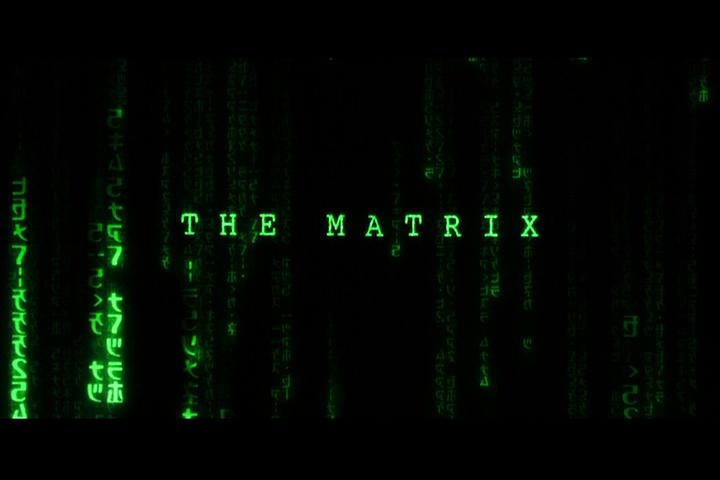
\includegraphics[width=0.5\linewidth]{fig/eeeb9f515ea2062442a75b17.jpg}
\end{figure}

题目的后半部分是Revolutions. 不光是革命,还是复数。有必要理解一下这个复数所代表的多重革命:

1、自由人类对Matrix非选择性工作体制的革命。

2、无目的程序对Matrix删除制度的革命。

3、过期程序对Matrix强行安排固有命运的革命。

4、人类内部对于Matrix性质认识的革命。

每一种都会在后面详细解释,这里就不多讲了,其实在这里也讲不出什么实质来。

\begin{figure}[htb]
\centering
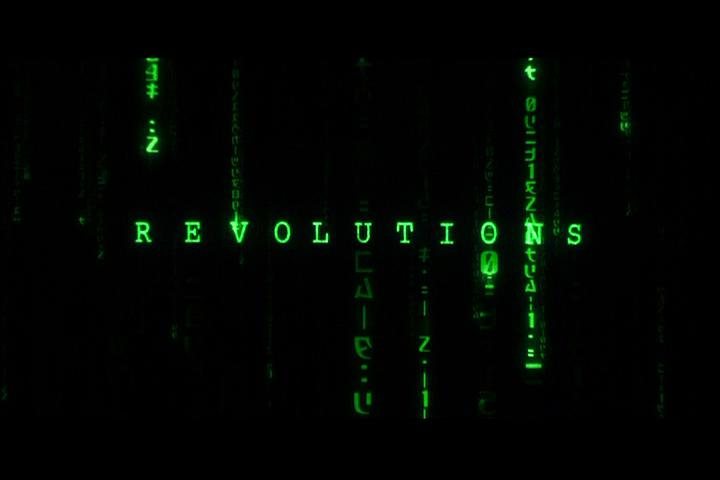
\includegraphics[width=0.5\linewidth]{fig/0b330eb35d354ba7d9335a17.jpg}
\end{figure}

金色,灵魂的颜色。哲学家音轨里两位教授都是这么认为的。金色的爆炸就意味着灵魂的诞生和飞速发展。从电影看来,金色是特指机器的灵魂,人类则缺少这么灿烂的光芒。Neo在瞎了眼之后可以感觉到被人类视为仇敌的机器,却看不到自己的另一半Trinity,就是最好的证明。

\begin{figure}[htb]
\centering

\includegraphics[width=0.5\linewidth]{fig/9ad10e2411b6d033c8955917.jpg}
\end{figure}

吧友一杯冰牛奶曾经指出这是数学中的分形结构,也具体指出了是哪一种,我认为哪一种不重要,而是分形所表达的意思。分形结构对于没有接触过这个方面的人(我就对分形一无所知)来说,最大的特点就是自我中有自我,生生不息。你可以从这个图形的任何一部分中找出这个图形本身。就像两面正对着的镜子,你可以从任何一面镜子(包括镜子的像)中找出其余任何一面镜子的像。于是我认为这里导演想要表达的意思就是,机器在发展的过程中不断地产生自我,完善自我。虽然更为精致、更为智慧,但这是一再重复着的、没有本质变化的进化。

\begin{figure}[htb]
\centering
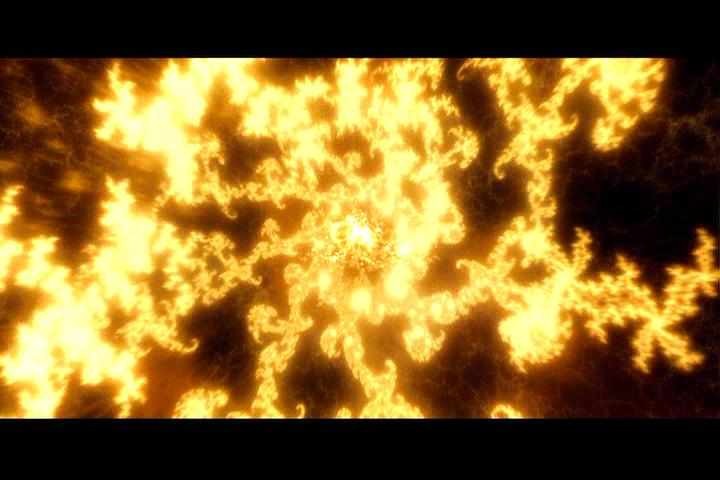
\includegraphics[width=0.5\linewidth]{fig/84bda8ec1f016a2762d09f11.jpg}
\end{figure}

这就是机器城啊!Neo在Logos号向下俯冲的时候看到的就是这个景象。从这以后,前伸的镜头开始倒退,我们看到的就不再是机器灵魂的灿烂金光,而是Matrix的代码。如果说第三部的开头代表的是AI的成长,这里无疑意味着“第二次文艺复兴”(the Second Renaissance),机器建立了机器城,和人类打了一仗,然后就靠着Matrix安逸地生存。

\begin{figure}[htb]
\centering
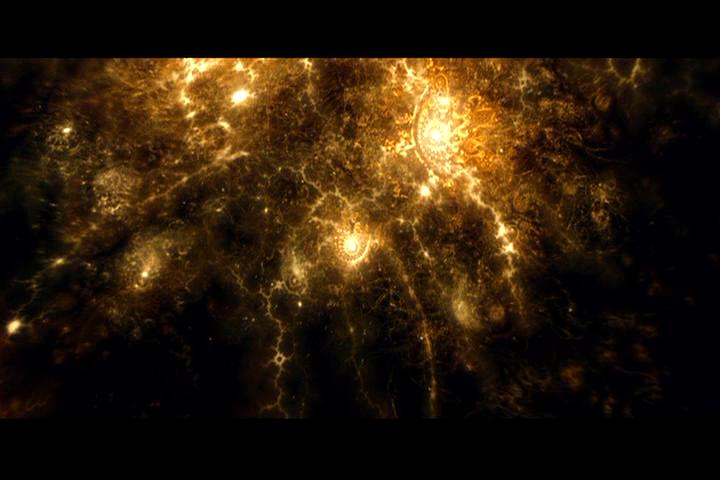
\includegraphics[width=0.5\linewidth]{fig/3c8e8b13f5356bd0f7039e11.jpg}
\end{figure}

这里就是人类历史上的最大转折点“第二次文艺复兴”。之后,绝大部分人类生活的世界。我要指出的是,这个世界没有机器的外在压迫,人类要对抗机器的唯一正当理由就是为了Zion 25万居民的生存,还有就是对Matrix内部人类社会发展的限制。这限制就是:二十世纪初人类发明AI,AI发展到和人类对抗的地步,人类战败后在Matrix里度过了大约6个世纪(前两个失败版本还未计算进去),所以外在世界至少是26世纪了。即便是Morpheus所说的22世纪,Matrix也已经对人类自然发展造成了一个巨大的障碍。不过这不应该是我们要把机器干尽杀绝的理由,罗素在《西方哲学史》中说亚里士多德延缓了科学的发展,但是他仍然把亚里士多德当作大哲学家,大科学家。同理,机器也不该因此被称作奴隶主。况且,科学是双刃剑,任由人类自由的飞速发展,还不知道我们是否能活到26世纪呢。

当然,这种“自由”的概念是黑客帝国官方网站上写论文的那些哲学家的思想,也是大多数人接受的“自由”概念。导演要表现的却是叔本华所说的绝对自由,也就是第三种自由,不光是“我能做我想做的”,而是“我要不受限制、随意地做我想做的”。这句话非常难表达,我这么说其实已经陷入了叔本华所说的循环中。要完全理解这第三种自由,还是看看叔本华本人《悲观论卷集》中在《伦理学的两个基本问题》里对概念的规定。这里我只能这么说:“绝对自由是无序的,不可预测的。”这个理论会在后面由Smith指出。

\begin{figure}[htb]
\centering
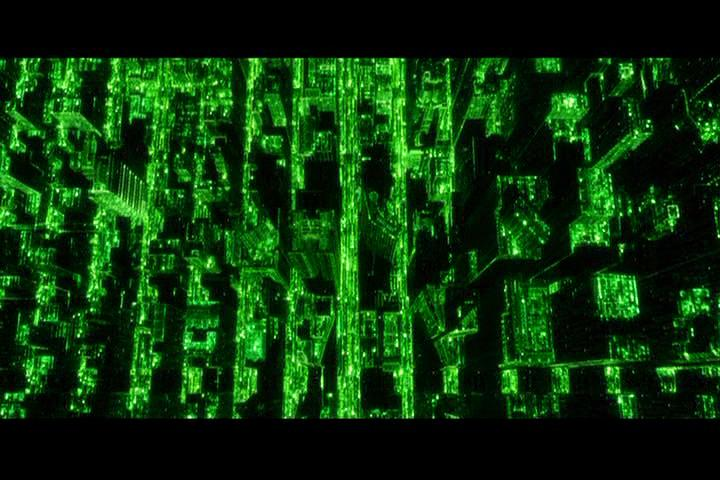
\includegraphics[width=0.5\linewidth]{fig/1f716227f5c2fe03918f9d11.jpg}
\end{figure}

这个图形非常有趣。要知道导演Wachowski兄弟(也许是姐弟了)来自芝加哥,酷爱篮球,偶象是飞人乔丹,最喜欢的篮球队就是芝加哥公牛队。几乎在每个国外的黑迷论坛上都提到这个图形的来历,那就是芝加哥公牛队的标志。同时,导演俩还把Mega City设计为这个标志的形状。无论是第二部的高速公路还是最后Neo和Smith决战的大街,都设计在了这张地图上。这也看出了导演俩对于符号的热爱。(导演俩在拍电影前搞了多年的漫画,漫画是最崇尚符号使用的。现在两人拥有一家漫画公司Burly Man Entertainment,Burly Man就是当初拍摄黑客帝国时用的替代名)

\begin{figure}[htb]
\centering
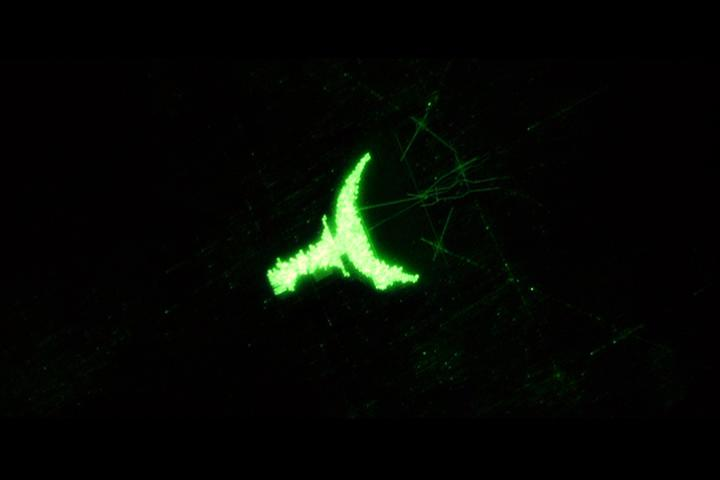
\includegraphics[width=0.5\linewidth]{fig/245732fa9999af1ea8d31110.jpg}
\end{figure}

Matrix在屏幕中,屏幕的意象是明白到不能再明白的了。屏幕中的就是拟像,还要再提一下已经被我们引用过成千上万遍的鲍德里亚的名言:“拟像不能使我们想象现实的存在,而本身就是虚拟存在的真实。”这里有必要提一下《十三楼》,在黑客帝国两个月后上映实在是太可怜了,本身也是一部很好的作品啊。除了结尾以外,对笛卡尔的“我思故我在”解释是很精辟的。

这里提出来说呢,是因为《十三楼》中的虚拟世界里,连人类都是完全虚拟的。这就更有针对性了,电影中把这些虚拟人也认作是人,和鲍德里亚所表达的意思一致。不过黑客帝国对鲍德里亚哲学解析的精髓不在这里,而在第一部中Cypher和Trinity的对话中。导演使用他的“虚拟现实”化解了昂格尔(Peter Unger)的“真实的价值”(value of the truth)对诺齐克(Robert Nozick)“经验机器”(the experience machine)的攻击。到第三部,导演就不再对“虚拟现实”进行更深入的解析,不过符号的拿手戏还是没有放下。

\begin{figure}[htb]
\centering
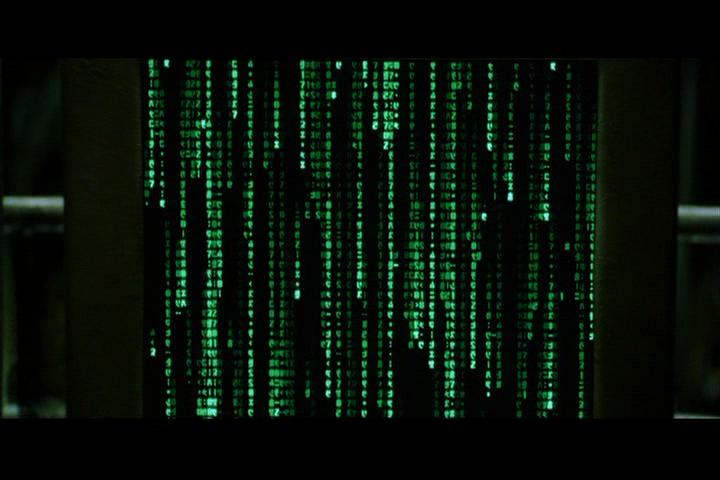
\includegraphics[width=0.5\linewidth]{fig/a698838bba0ca1d3fd1f1010.jpg}
\end{figure}

\begin{myquote}
AK: I got nothing, sir. No sign of Niobe or Ghost. Nothin' but blue pills.

Mauser: Should we jack in and try to contact them?

Roland: It wouldn't matter. My gut says they're down.

Mauser: Then we should start back.

Roland: No. If that ship can still fly, then we need it.

Mauser: I was afraid you were gonna say that.
\end{myquote}

这里解释一下他们的话,那句blue pill就是指代有机会出来但没有出来的人,他们没有勇气接受现实的改变,就和机器一样。其实大多数人都是如此,搞不好我就是一个blue pill。

Roland说:“只要那艘船还能飞,我们就需要它。”其实他们需要的是Logos的EMP。这里要说一下,EMP是装在飞船上,拿不下来的。而且根据每艘船的铭牌,这些船都是机器城制造的,所以说人类没有能力制造更多的EMP来对抗机器。而且电影里的EMP和我们现在不同,我们现在都已经有能力对付EMP了。说EMP和现代的不同还有另一个原因,《第二次文艺复兴》中,人类对机器使用核弹但是收效甚微,核弹爆炸也会产生EMP的效果,足以说明当时的机器就有能力对抗EMP了。机器造这些新式EMP给人类来攻击自己的目的会在后面解释。而Zion城其实也是机器留给人类的,是上一代救世主救出23个人之后就把他们带到Zion,以前也有fan fiction说Zion是以前的人类军事基地。所以说Zion的来历并不重要,我们有足够的理由认为Zion存在着。

\begin{figure}[htb]
\centering
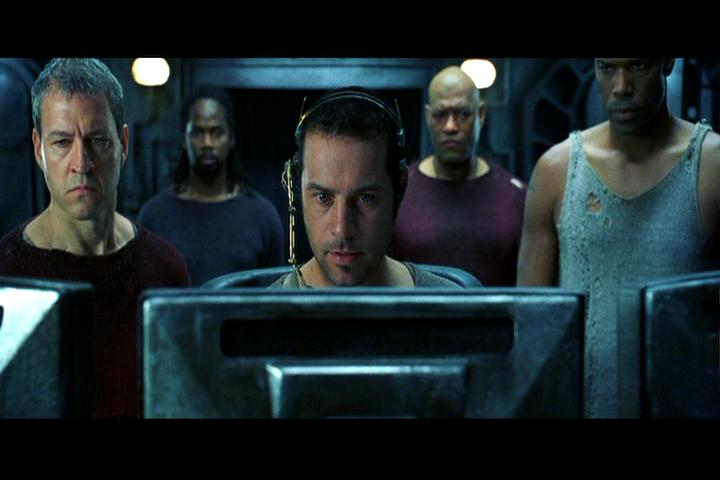
\includegraphics[width=0.5\linewidth]{fig/17e9a71eb5c1f41f41341710.jpg}
\end{figure}

\begin{myquote}
Roland: Search every pipe, every hole, every crack we know. Sweep as wide as possible, as fast as possible.

AK: Captain, these lines are crawling with calamari.

Roland: Then the sooner we find them the better.
\end{myquote}

现在说一下这些人的名字:

船长Roland, 这个名字可能源于查理曼大帝的法兰克管家。在史蒂芬金的作品The Dark Tower中,他被形容为一个枪手。而他的手下正好都以武器为名字。

大副Colt, 柯尔特自动手枪,喜欢枪械的朋友一定不会陌生。

接线员AK, 连对武器一窍不通的人都应该听说过著名的AK47。

船员Mauser, 德国毛瑟枪,简陋而原始的枪,用黑人来演自然是表示原始的力量。

医护员Maggie, 是Margaret的缩写,那是一本著名的关于枪械武器的杂志。

\begin{figure}[htb]
\centering
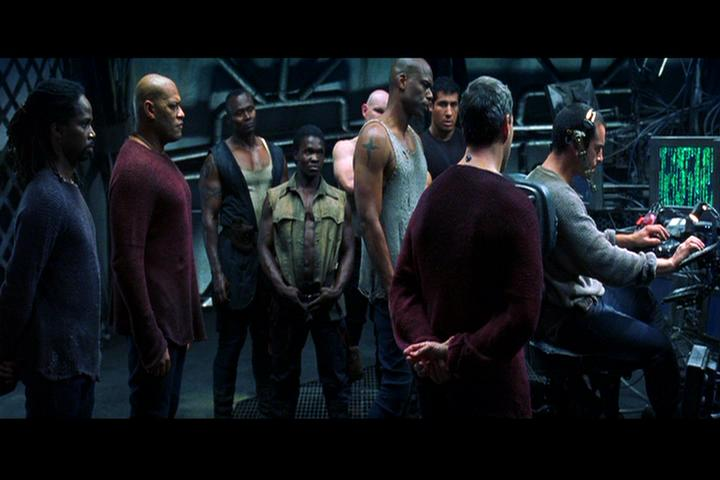
\includegraphics[width=0.5\linewidth]{fig/84bda8ec1f006a2762d09f12.jpg}
\end{figure}

\begin{myquote}
Maggie: Thought you could use something to eat.

Trinity: Thank you.

Maggie: Any change?

Trinity: No. How's he?

Maggie: He's going to be fine, at least until he wakes up.

Trinity: What do you mean?

Maggie: The captain has some questions for him. He better have some good answers. You see these cuts? I think they're self-inflicted.

Trinity: Why?

Maggie: VDTs, maybe. I don't know. But like I said, the answer had better be good.
\end{myquote}

我在第一次看这部电影的时候,没有去查这个VDT的意思,想当然的认为VDT是精神分裂之类的病症。仔细查了之后才知道这是导演兄弟自己编出来的词汇,意思是virtual delirium tremens,虚拟震颠性谵妄。本来是有delirium tremens这个医学名词的,其最明显的症状就是“幻觉”。

在这部片子的评论音轨(哲学家音轨)中,Ken Wilber和Cornel West都提出这第三部是三部曲的循环部分,连接部分。第二部在这里结束,第三部就在这里开始。而且导演俩也比前两部更注重平衡和阴阳,以尽可能和谐的构图来表现这部电影,画面非常对称,对单个人物的特写全都构建在镜头的半面,几乎是完美的平分画面。这一点在导演俩的处女作《Bound》里就做得非常出色。

这里既然出现了Trinity, 那就再谈一谈Trinity和the One的关系。trinity的拉丁文变体为tria iuncta in uno,那就是三溶于一。先知说过the One之路是由众人组成的,Trinity就是最重要的部分。Ken Wilber和West博士都在音轨里说过,没有Trinity的the One是不完整的。

\begin{figure}[htb]
\centering
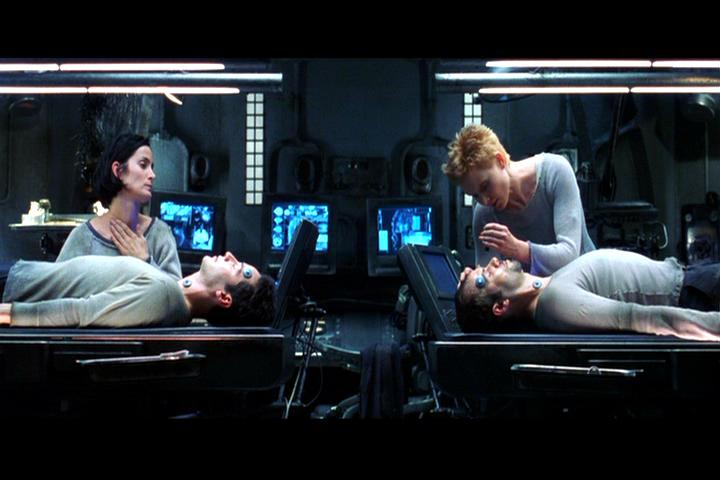
\includegraphics[width=0.5\linewidth]{fig/3c8e8b13f5346bd0f7039e12.jpg}
\end{figure}

\begin{myquote}
Morpheus: Roland. I'd like to run another search through the Matrix.

Roland: For what?

Morpheus: For Neo.

AK: How can he be in the Matrix, sir? He's not plugged in.

Morpheus: Please, for me.
\end{myquote}

Morpheus不愧是梦神,一下就明白了Neo的精神到了另一个世界。但是我们要注意的是,Neo的精神和身体并未分离,即便Neo到了另一个世界,他还有一个“自我形象”可以控制。正如世界本质的几个假说造物说、计算说等等,无论你身体的本质如何改变,这始终是你的身体。

\begin{myquote}
Maggie: This is what keeps bothering me.

Trinity: What?

Maggie: His neural patterns don't read like someone who's in a coma. The strange thing is, I see these patterns all the time.

Trinity: Where?

Maggie: On someone jacked in.
\end{myquote}

本来Morpheus这么一说,外加Maggie这么一补充,我们都会以为Neo就在Matrix中,导演却安排AK这么回答:

\begin{myquote}
AK: The big bubkis. Nada. He's not in there.

Colt: Sir, we've got the projections!

Roland: How long?

Colt: Based on the point of entry and the [past] speed it looks like the machines will be inside of Zion in just under 20 hours.

AK: Jesus H. Christ.

Roland: All right, let's move with a purpose. AK, get upstairs, I want you on holographics. [Colt,] Mauser, I want forward and aft guns manned at all times. And make sure we are running on as few pads as possible.

Colt: Yes, sir.

Link: Hey. Hey! We got a call. Operator. It's Seraph.

Seraph: I bring word from the Oracle. You must come at once.
\end{myquote}

我们敬爱的同胞Seraph出现了,做事雷厉风行,一句话就挂电话。程序的目的啊,不让他废话一句,看来他受着无尽的限制。但没有了规则,程序还能存在吗?我们在这里要回忆一下Seraph的程序目的,“保护最重要的”。再看他接下来的行动,就会明白Matrix现在最重要的是什么。

\begin{figure}[htb]
\centering
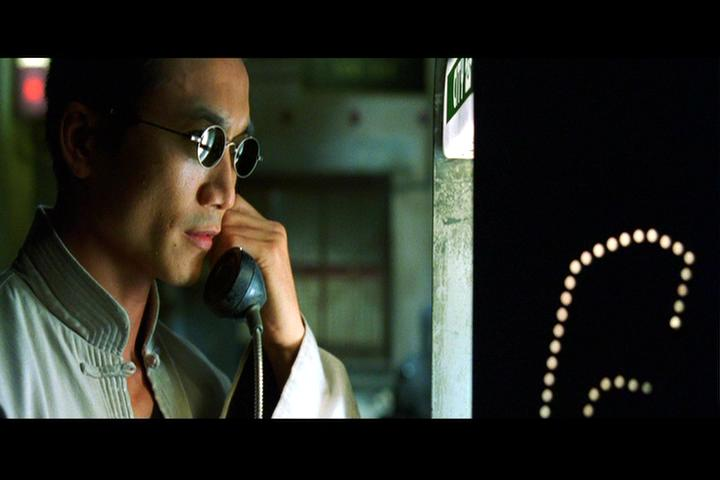
\includegraphics[width=0.5\linewidth]{fig/1f716227f5c3fe03918f9d12.jpg}
\end{figure}

\begin{myquote}
Sati: Good morning.

Neo: Who are you?

Sati: My name is Sati. Your name is Neo. My papa says you're not supposed to be here. He says you must be lost. Are you lost, Neo?

Neo: Where am I?

Sati: This is the train station.

Neo: This isn't the Matrix?

Sati: That's where the train goes. That's where we're going. But you cannot go with us.

Neo: Why not?

Sati: He won't let you.

Neo: Who won't let me?

Sati: The Trainman. *whispers* I don't like him, but my papa says we have to do what the Trainman says, or he will leave us here for ever and ever.
\end{myquote}

揣摩一下这里的话吧,有人指出过Sati这里说的“早上好”很有意思。这里有时间吗?有时间的话,为什么是早上呢?接着,Sati就明白的说出Neo是谁,又是一个疑点。看看这张图,她身边一圈光环。再看一下Sati这个名字吧,是指印度教妻子殉夫的传统,充满祭祀、牺牲的意思。还有一个意思是梵语的“being”,就是本质、存在、生命这些意思。而且Sati还是印度教的一个神。

叔本华、尼采都是很崇尚印度教的。导演俩也是如此,他们原本在George设计的飞船中起了些Vishnu、Brahma这样的名字。

据说梵天产生此世界,是由于某种错误而成的。为了补偿自己的过失,它便置身于这个世界之中,一直到设法能补偿了为止。如此说明了万物的起源,是多么值得称道!依照佛教的教义,世界的产生,是由于一些莫名其妙的骚扰,打破了涅盘天地的神圣的宁静。

我这里引用一句拉丁谚语:Prudens futuri temporis exitum caliginosa nocte premit Deus.(智慧的神用黑暗卷起未来)

所以导演一直给我们传达一个信息:信仰单一真神,信仰那完美的力量,就是一种逃避。

\begin{figure}[htb]
\centering
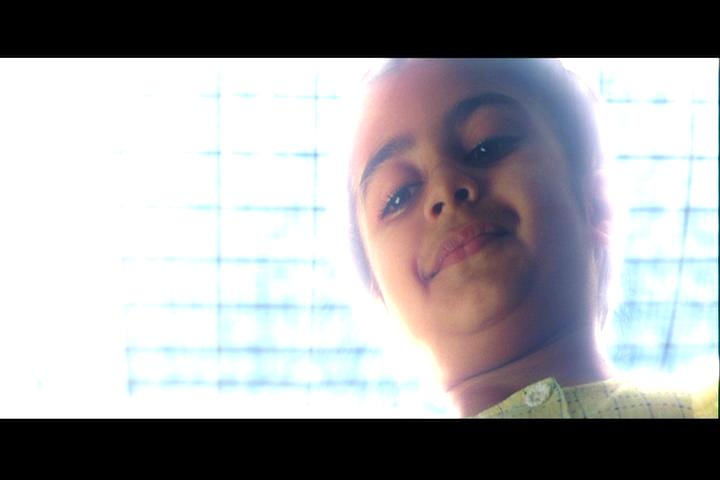
\includegraphics[width=0.5\linewidth]{fig/cce0b3b70bb105f431add112.jpg}
\end{figure}

这里还要注意一句台词,leave us here for ever and ever。没有用forever, 而是for ever and ever,导演还特别让Sati突出了这部分。这又是一语双关(为什么要用“又”呢?因为neverwin达人在前两部里解释了很多一语双关的例子),意思就是:“你被留在这里是因为过去的事。”比较了解黑客帝国的朋友应该明白这和法国人是什么关系。我们知道法国人掌控Matrix的信息,并以因果律(并非霍金所说的纯物理因果律,这一点会在后面提到)推测过去发生了什么。所以我们每次遇到法国人,他都会准确无误的知道我们来的目的,甚至是一点细节。比如后面我们会看到,法国人一看到Seraph来了就说先知一定找到了新的躯壳。这里法国人就是为了“过去的事”把Neo囚禁了,是哪一件事我们很清楚,呵呵,几分钟就把法国人好不容易培植出的势力干掉了,他能不生气嘛。

另外再说一下Sati的身份,很多人认为Sati是下一代先知。我认为这似是而非,一来Sati是无目的程序,把她分类本来就不对;二来Sati确实有先知的能力。后面我们会看到,Trainman根本不认识Neo, 而Sati却已经知道Trainman不会让Neo走了。我们暂且说Sati是一个有先知能力(还有其他能力,像是控制天气)的无目的程序。

注意这张图中这个火车站的名字,Mobil Ave, 这个Mobil就是Limbo的乱序词。Limbo的意思就是世界间的世界。在但丁的神曲中,Limbo被描述为九层地狱的第一层,里面的人不受折磨,享有无尽的空虚。不相信神,也不反对神的人就会待在这样的地方。而在Matrix中,我们明白,既不相信神也不反对神的人是真正理解神的人、知道神的立场的人。

\begin{figure}[htb]
\centering
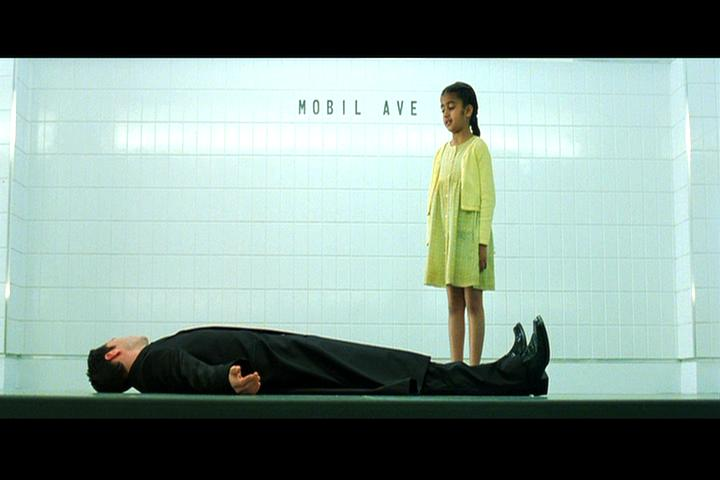
\includegraphics[width=0.5\linewidth]{fig/e36b4a3679b53bdda3cc2b19.jpg}
\end{figure}

\myparsep

马上就要去见先知了。先看看先知公寓那里的情况,看看墙上的涂鸦(可以在黑客帝国官方网站的Zion Archives找到),下面那张图中写的是guts。记得前面Roland说了什么吗?他说:“My gut says they're down.”这一点秉承了叔本华的直觉主义,在先知这里也不例外。我们常说先知的能力可以用因果律、全定论来解释,而叔本华最讨厌的黑格尔也认为“时间是我们看不全面而产生的幻觉”,但是这样一来就无法解释先知只能“believe”未来的相关台词。导演就暗示我们,这不是完美的因果律和全定论,也不是令人不愉快的宿命论,而是我们的直觉。

这一点我之所以不在Roland那里就指出,是为了避免大家误会Roland是直觉主义,而先知是全定论,其实二者都是基于直觉主义的。当然,长期研究人类情感的先知要可靠得多。

\begin{figure}[htb]
\centering
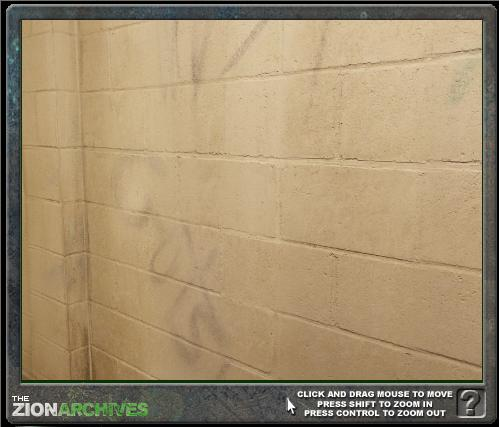
\includegraphics[width=0.5\linewidth]{fig/43ead53fab4bbcc27c1e7125.jpg}
\end{figure}

看一些墙上的涂鸦,这些不像guts这样重要,不过仔细看还是很有趣的。这张没有什么隐藏的意思,就是peace。我们知道先知要的就是peace,先知believe的就是peace。

\begin{figure}[htb]
\centering
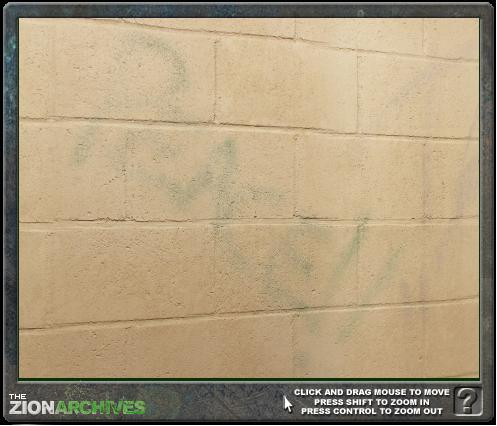
\includegraphics[width=0.5\linewidth]{fig/27d5d1a2c52f2dadcaefd05a.jpg}
\end{figure}

下图上方的图形就是无政府主义的标志,A外一个圆圈,其实V for Vendetta的标志就是从这个标志来的。

\begin{figure}[htb]
\centering
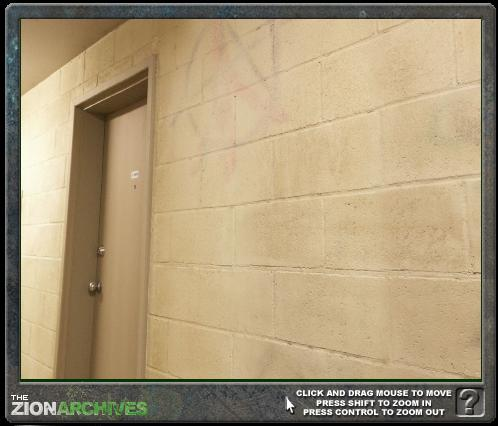
\includegraphics[width=0.5\linewidth]{fig/45c00df4fb76d7ef7709d75a.jpg}
\end{figure}

估计写到这里就已经有人认为我找得过头了。就拿guts来说,有人会问:“这么重要的标志会藏的这么隐晦?”这么说吧,对于一般的观众来说,先知预知未来的能力是不必解释的,这个标志自然就不重要了。但是对于我们这种试图分辨先知是全定论还是直觉主义的人来说,这个标志也不如Nebuchadnezzar飞船的铭牌寓意对于虔诚的基督徒来说更隐晦。

整个《黑客帝国》系列,正如叔本华称自己作品“不是写给老百姓看的”一样,不是给普通的影迷或是影评人看的。喜欢《黑客帝国》的哲学家们也不愿意更多的人喜欢《黑客帝国》,因为他们认为只看特技的人不配喜欢《黑客帝国》, 以至于用过于复杂的理论来讨论黑客帝国。一个例子就是哲学家David J. Chalmer甚至在一篇讨论《黑客帝国》的形而上学理论的文章里生造了一个有关存在主义的哲学术语“envatted”(非原存在,虚拟之类的意思,类似缸中之脑的处境,字典上是查不到这个词的)。在那之后,很多哲学家受他的影响,凡是可以用envatted这个词的时候,就不用更加大众化的词语来描述了(大家可以去搜索一下,这个词三分之一的使用语境已经和Matrix无关了,成为了一个正宗的哲学术语),就是要把那些普通影迷拒之黑客帝国的门外。

但是这样做有个副作用,由于高深的理论被哲学家们屏蔽了,大众眼里的《黑客帝国》还不如原本十分之一那么高深(这里的大众已经是指对黑客帝国颇有研究的人了,以全体观众作为整体来看,黑客帝国完全是被糟蹋了)。这一点是导演不希望看到的,我也觉得这个情况很糟糕,所以才写这篇文章,我想neverwin也是因为这个原因吧。虽然我们这么做也是导演不希望看到的(导演希望观众自己去思考,而不是像我们这样给读者们灌输我们自己的想法)。

当然了,上面这段可以算是废话,但正如Smith所说,我需要justify the existence of the essay。不过有一点各位要确定的是,导演绝对比我描述的睿智得多。

废话不说了,直接进入和先知的谈话。

\begin{myquote}
Oracle: Morpheus, Trinity. Thank you for coming. One thing I've learned in all my years is that nothing ever works out just the way you want it to.
\end{myquote}

这句太有趣了,我们知道先知做事的方式就是安排未来,Neo打碎花瓶就是一个例子,而先知本人却说未来从来不像自己期望的那样。这一点又是叔本华的理论:“时间乃一主动力,将每一刹那间,我们所掌握的一切事物,都变为无,而丧失其所有的价值。”所以说无论先知做什么,总是没有价值的。只要时间存在,“价值”这个词是没有含义的。先知如此低沉的说出这个理念,就是因为这种价值观正是Matrix的大敌Smith的哲学。

\begin{myquote}
Trinity: Who are you?

Oracle: I'm the Oracle. I wish there was an easier way to get through this, but there ain't. I'm sorry this had to happen. I'm sorry I couldn't be sitting here like you remember me. But it wasn't meant to be.
\end{myquote}

有人说先知解释自己的样貌变化是欲盖弥彰,但事实上,先知的shell被出卖是十分重要的,正是“革命”一词的导火索。说到换演员的问题,其实原剧本就要求换演员了,只是Foster演得太好而让她继续演下去的,不幸的是我们亲爱的先知去世了。

\begin{myquote}
Trinity: What happened?

Oracle: I made a choice, and that choice cost me more than I wanted it to.
\end{myquote}

这一点和法国人的观点也很相似,cost也是选择的一个重要的环节。叔本华举过一个很古老的例子,一头驴放在两堆相等的食物中间,这头驴最后会活活饿死。因为两个选择的代价是相同的(不一定是付出,获得也是一种cost, 不过电影里指的仍然是付出),于是这头驴就无法作出选择。叔本华在举了这个例子之后还说人也是一样的。

\begin{myquote}
Morpheus: What choice?

Oracle: To help you to guide Neo. Now, since the real test for any choice is having to make the same choice again, knowing full well what it might cost --- I guess I feel pretty good about that choice, 'cause here I am, at it again.
\end{myquote}

在知道了选择的代价之后,再作出这个选择是困难的。我可以拿那个驴子的例子来解释,对于那头驴来说,两边的选择是一致的。这也是先知的处境,不帮助Neo违背自己的意愿并造成Zion 25万人的死亡,帮助Neo可能会造成极大的破坏。先知作出了帮助Neo的选择是因为她believe。同理那头驴只要原本倾向于左或是右(相当于Believe)就可以不被饿死。

\begin{myquote}
Trinity: Do you know what happened to Neo?

Oracle: Yes. He's trapped in a place between this world and the machine world. The link is controlled by a program called the Trainman. He uses it to smuggle programs in and out of the Matrix. If he finds out where Neo is before you get to him, then I'm afraid our choices are going to become difficult.

Trinity: Why?

Oracle: Because of who the Trainman works for.

Morpheus: The Merovingian.

Oracle: He has placed a bounty on your lives. You must be careful at all times. Seraph knows how to find the Trainman, he will go with you. For years, he has protected me. I hope he can do the same for you.
\end{myquote}

还记得Seraph的目的吗?那就是保护最重要的东西,这个最重要的东西不一定就是先知,以前法国人有势力的时候,他保护法国人;当先知成为最重要东西的时候,他就保护先知;这时,Morpheus和Trinity承担拯救Neo的任务,那他们就是最重要的;后面我们还看到他保护Sati, 正说明Sati的重要性。

\begin{myquote}
Seraph: Please, follow me.

Morpheus: Oracle.

Oracle: I know, Morpheus. I can see you're filled with doubt, clouded by uncertainty.

Morpheus: After everything that's happened, how can you expect me to believe you?

Oracle: I don't. I expect just what I've always expected. For you to make up your own damn mind. Believe me or don't. All I can really tell you is your friend's in trouble and he needs your help. He needs all our help.
\end{myquote}

这里很有趣,先知最初的作用就是获得人类的信任,这里她开始耍无赖了:“我又没叫你相信我!”事实上,在先知的眼里,无论是相信她还是不相信她,都可以被她利用。这里又有一句双关语damn, 这个词neverwin解释过了,就是诅咒,控制之意。也就是说“你要决定的是被控制的思想。”这个控制Morpheus的就是先知本人,就和她让Neo打碎花瓶一样。

先知的耳环上是太极图案,香烟牌子是Double Destiny, 茶杯上是莲花图案。仔细看电影的人应该都有印象,我就不一一截图了,给一张意思一下:

\begin{figure}[htb]
\centering
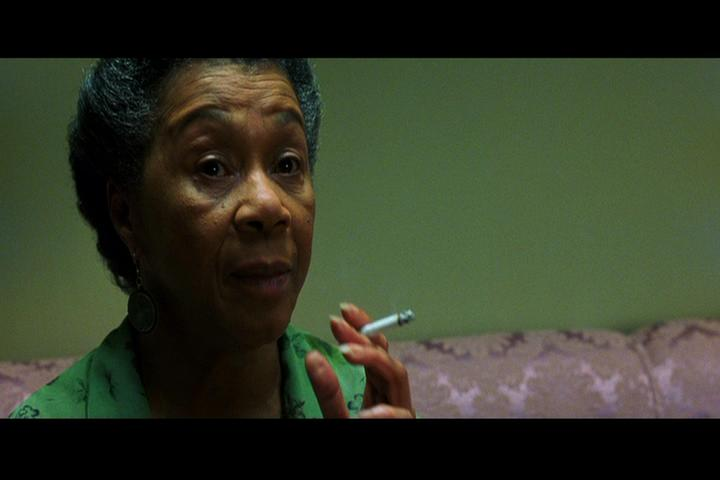
\includegraphics[width=0.5\linewidth]{fig/14a938db9f7b7466d0164e8c.jpg}
\end{figure}

太极代表平衡和阴阳,有Neo就有Smith,充分证明Smith作为Neo对立面是由先知造成的。当然,有人会说这是设计师为了平衡方程式而造成的。但是根据设计师在第二部的说法,Neo属于哥德尔命题中的逻辑外真理,是不能用数学方式解决的。事实上,先知这时“打破平衡”的方式正是“平衡”Neo和Smith(并非无情的数学方式,而是先知的拿手好戏,心理方式,证据是Neo和Smith在能力上的不平衡性),系统把全系统的逻辑外真理归结于Neo(易于管理),一旦Neo被平衡,这个逻辑外真理就演变为“关系”,而非“值”。但是换一个角度看,先知“打破平衡”正是为了真正的平衡,就是最后的和平。“和平”就是一个观众可以期待到的最佳结果,除非这个人还没有摆脱极度人类中心论。

Double Destiny同样代表着和平。鲍德里亚说“利益的平衡就是平衡的利益”,设计师所设想的(也是实现了的)平衡建立在了不平衡的利益之上,以力量来弥补这种平衡上的不足,这是机器中心论。先知要做的就是改变这种渗透了力量的利益平衡,所以先知要考虑机器和人类双方的问题,是double destiny。

莲花在印度教里和守护神Vishnu有极大的联系,对他我就不仔细说了,Vaishnava认为Vishnu是至高神,Smarta认为Vishnu只是梵天的一个化身。所以多说反而麻烦,很容易混淆。不过只要知道他是“守护神”就够了,完全可以诠释先知的立场。

neptuneneo兄跟我说《黑客帝国》也是很不错的爱情片,他指的是Ghost对小崔很东方的暗恋。仔细看看小崔和Neo的爱情也很有味道,该热烈就热烈,该含蓄就含蓄。这里一听Seraph要带他们去救Neo,小崔立马转身跟去了,根本没有考虑先知以前对他们撒的谎。这里还是老莫沉得住气。情爱是疯狂的,友爱是理智,父爱是形而上学的。(叔本华语,马上就要在Rama出场后讲一下这个父爱)

另外讲几点有趣的小细节:

先知的香烟盒上有一段文字很有趣:“烟草会产生一些序列,这些序列会造成胸口疼和突发心脏病。”很有Matrix味道吧。

剧组为了纪念老先知的去世,特地在场景里加了一个天鹅形的钟。

先知在这里坐的位置是第一部里一个念佛经的小孩坐的地方,老莫和小崔站在了玩勺子的小孩坐的地方,Seraph站的是第一部里给Neo开门的那个领路人的地方。

\myparsep

我们回到火车站,看看这些对话里有什么值得学习。(为什么不说“值得注意”呢?因为光注意是不够的,黑客帝国应该是拿来学习的东西)

\begin{myquote}
Sati: Are you from the Matrix?

Neo: Yes. No. I mean, I was.
\end{myquote}

Neo还在强调时间,说明他还没有掌握时间。但是他对时间也有直觉,他预感到了大楼的爆炸,预感到了乌贼。但是他不能控制这种能力,这种看透一切的能力。(黑格尔说“时间是一个人无法看透一切而产生的幻觉”)根据全定论或是因果律,一切皆注定。我很不明白的是,为什么有这么多人认为一切都是偶然呢?不管别人,反正导演相信一切注定,叔本华相信一切注定,对我来说足够欣慰了。

\begin{myquote}
Sati: Why did you leave?

Neo: I had to.
\end{myquote}

这是典型宿命论的论调,或是悲观面对全定论的态度。Neo刚刚才消极地讨论时间,这里消极地讨论命运也是必然的。其实Neo的思想进步正是导演的哲学学习历程,我可以万分肯定这一点,因为我本人就是这样。在看到全定论本质之前看到全定论的现象,消极的悲观论调是不会少的,除非是乐天派。(乐天派喜欢哲学吗?)

\begin{myquote}
Sati: I had to leave my home too.
\end{myquote}

这一句其实是很厉害的,“我也是不得不离开家”,就是说对Neo来说,Matrix才是他的家。或者我们可以再老套一点,谈笛卡尔的身心二元(对黑迷来说都审美疲劳了)。我在这里分的身心二元和笛卡尔的并不一致,是把Neo分为人和程序。(画外音:看起来好像和笛卡尔一点没关系嘛!)这里的程序是身,人是心。Neo是以人的思维,程序的能力在做事。Sati这句话是对Neo的程序身份说的,因为Sati并不明白人类的思维,我们在后面看到先知在教Sati什么是“爱”。

\begin{myquote}
Rama-Kandra: Sati! Come here, darling. Leave the poor man in peace.

Sati: Yes, papa.

Rama-Kandra: I'm sorry, she is still very curious.
\end{myquote}

这个“好奇”是很重要的,这是任何有意识的物体所必备的特质。

\begin{myquote}
Neo: I know you.

Rama-Kandra: Yes, in the restaurant of the Frenchman. I am Rama-Kandra. This is my wife Kamala, my daughter Sati. We are most honored to meet you.
\end{myquote}

Rama是Vishnu一个化身的名字,也可以看出他和先知的关系不一般了。Kamala是一个印度神Lakshmi的一个别名,Vishnu的妻子(其实她和莲花关系更大,Kamala的意思就是“she of the lotus”)。由于导演有糅合基督教野史和古希腊神话的前科,看来他们对印度教是最尊敬的。叔本华、尼采、肯·韦伯无不欣赏印度教(叔本华在印度待了好几年研究印度教呢),因为印度教就是一种哲学,而不是一种控制人的方式。

\begin{myquote}
Neo: You're programs.

Rama-Kandra: Oh, yes. I'm the power plant systems manager for recycling operations. My wife is an interactive software programmer. She is highly creative.
\end{myquote}

看看这些程序是干什么的!多么重要的程序啊!Rama管着Matrix人口的更新换代,Kamala管着人类之间的交流。而且两者都和救世主有着莫大的关系,Neo醒来时遇到的机器就是Rama (起码也是他管理的吧)。Neo的超能力和“交感”是密不可分的,所以说是Kamala赋予了他超能力。这对夫妇分明掌握着Neo的生死!而Neo又是系统不可或缺的部分,可见这两个程序的重要性。先知在《Enter the Matrix》游戏里说过,她的躯体是被她“最信任”的两个程序出卖的。那么他们和先知之间的关系也很明朗了。Rama释放Neo,而Kamala给Neo力量(当然,这也符合设计师原来的原则)。

\begin{myquote}
Kamala: What are you doing here? You do not belong here.

Rama-Kandra: Kamala! Goodness, I apologize. My wife can be very direct.

Neo: It's okay. I don't have an answer. I don't even know where ``here'' is.

Rama-Kandra: This place is nowhere. It is between your world and our world.
\end{myquote}

还是那句话,这里是Limbo,哪里也不是。可以说是世界间的世界,也可以说是地狱的第一层。

\begin{myquote}
Neo: Who's the Trainman?

Rama-Kandra: He works for the Frenchman.

Neo: Why'd I know you were going to say that?

Rama-Kandra: The Frenchman does not forget and he does not forgive.

Neo: You know him?

Rama-Kandra: I know only what I need to know. I know that if you want to take something from our world into your world that does not belong there, you must go to the Frenchman.

Neo: Is that what you're doing here?

Kamala: Rama, please!

Rama-Kandra: I do not want to be cruel, Kamala. He may never see another face for the rest of his life.

Neo: I'm sorry. You don't have to answer that question.

Rama-Kandra: No. I don't mind. The answer is simple. I love my daughter very much. I find her to be the most beautiful thing I've ever seen. But where we are from, that is not enough. Every program that is created must have a purpose; if it does not, it is deleted. I went to the Frenchman to save my daughter. You do not understand.

Neo: I just have never ...

Rama-Kandra: ... heard a program speak of love?

Neo: It's a ... human emotion.

Rama-Kandra: No, it is a word. What matters is the connection the word implies. I see that you are in love. Can you tell me what you would give to hold on to that connection?

Neo: Anything.

Rama-Kandra: Then perhaps the reason you're here is not so different from the reason I'm here.
\end{myquote}

“爱”只是一个词,重要的是其中的关系。这是连叔本华的对头黑格尔都同意的。问题是这个关系本身是否值得?叔本华认为除了同情,没有什么感情是不基于利益之上的。叔本华没有爱,只有性。这一点和设计师一样哦!(设计师的造型来自弗洛伊德)在《黑客帝国》里,并不是没有人持叔本华这种观点,Smith就是这个例子。印度一家的观点更像是尼采,虽然尼采也有很多让女人们很反感的言论,但是尼采是浪漫的。我们用一个“同理可证”就可以把尼采的“爱命运”转变为“爱爱情”。我们可以爱我们无法抗拒的命运,为什么不能接受这骗人的爱情呢?叔本华说:“世界是我的梦”。尼采说:“人生即便是梦,也要过得有滋有味。”这就是Neo和Smith的最大不同。

\myparsep

火车人出场了。

\begin{myquote}
Seraph: That's him.

Trainman: Get away! Get away from me!

Seraph: We don't want trouble.

Trainman: Get the hell away from me!

Seraph: We need your help.

Trainman: I can't help you. No one can help you!
\end{myquote}

追火车人这里可以看到一些有趣的广告牌,一些是赞助商的广告,比如说三星和Powerade的广告。最重要的还是下面图中那个Tastee Wheat。

第一部里Mouse问Neo有没有吃过Tastee Wheat的时候谈到了一个被我们黑迷称之为“麦片理论”的理论。这个理论其实很重要的,算是诺齐克“经验机器”设想的一个延伸。我们把味觉延伸出去,一切感官都在“麦片理论”的范围之下,甚至是自然定律也是。比如说你怎么知道在外面的世界里,你就不能飞呢?其实“麦片理论”可以解释一切这部电影里所谓的“科学问题”(虽然绝大部分不用这个理论也能解释)。

\begin{figure}[htb]
\centering
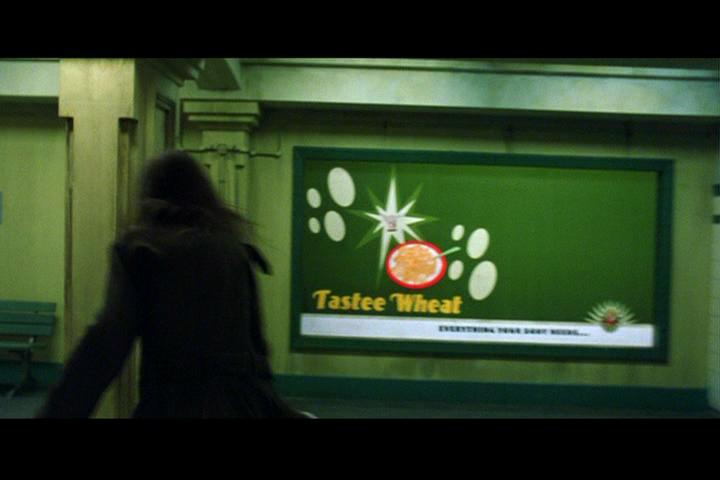
\includegraphics[width=0.5\linewidth]{fig/4000843531b7cf1190ef39a9.jpg}
\end{figure}

这里我要介绍一下一部我比较喜欢的电影《一九八四》(更喜欢小说,三大反乌托邦小说之一嘛),导演也是很喜欢这部作品的,我认为导演安排他们在吃饭的时候提出这个理论就是一种对《一九八四》的致敬。《一九八四》里有一段,主角温斯顿在吃饭的时候,对面一位仁兄说他们吃的那个东西看起来像是肉,尝起来像是肉,但却是豆腐做的(看得到“麦片理论”的影子吧)。neverwin也提到一点,Neo房间的号码101也是对《一九八四》的致敬(其中101房里的是一个人最大的恐惧)。导演兄弟编剧的新作《V字仇杀队》也有很多对《一九八四》的致敬,比如娜塔丽剃光头的镜头。有趣的是,在《一九八四》里反抗极权政府的温斯顿扮演者John Hurt,却在《V字仇杀队》中扮演了极权政府的头目。

这个很容易让人联想到那种兜售偷来的手表的人。不过不要以为这就是导演的意思。火车人一共有九块手表,而且时间各不相同,代表但丁所说的九层地狱。因为每一层地狱的时间都是不同的。

\begin{figure}[htb]
\centering
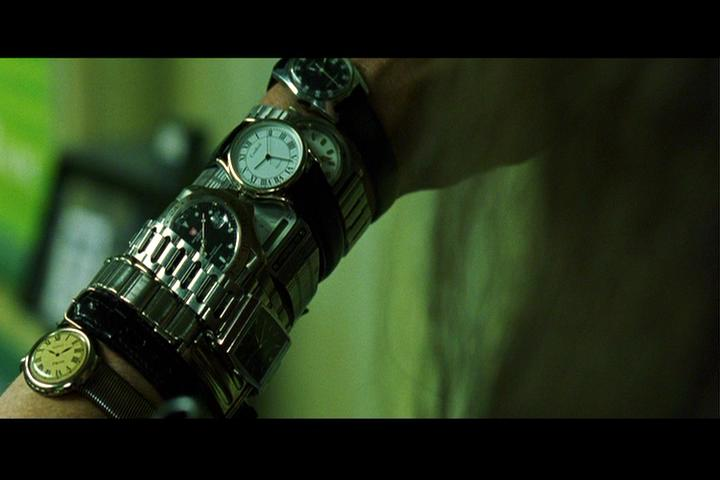
\includegraphics[width=0.5\linewidth]{fig/058d77c67f85e61b9d163da9.jpg}
\end{figure}

有人可能认为这是我在胡说,但是我可以证明哦。

下图是Rama在等火车时看手表,6点10分,正是上图火车人第一块手表显示的时间。两个镜头不是同时拍摄的,不要说这是巧合。再加上Limbo确实是地狱的第一层,应该没有什么异议和需要解释的地方了吧。而且这个6点10分也是有含义的。

圣经的撒母耳记下6:10:于是大卫不肯将耶和华的约柜运进大卫的城,却运到迦特人俄别以东的家中。

Rama不肯将Sati留在Rama的世界,却带到先知的家中。而且Sati本身也是一个契约,用先知的躯体换来的自由哦。

\begin{figure}[htb]
\centering
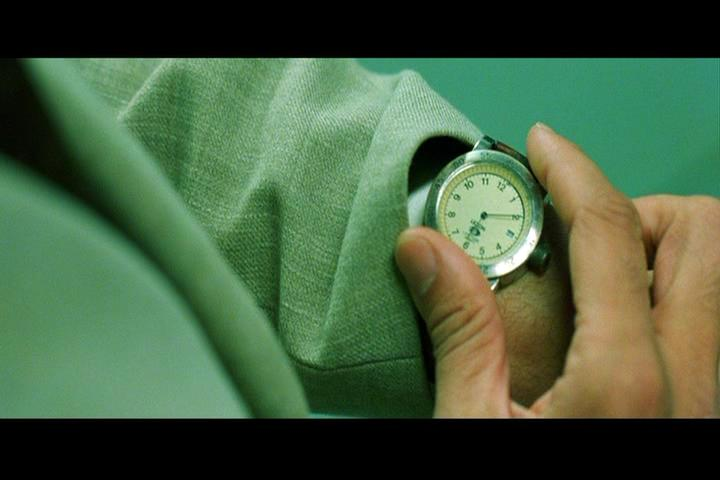
\includegraphics[width=0.5\linewidth]{fig/759c98255a5b746034a80fa9.jpg}
\end{figure}

\begin{myquote}
Neo: When is the train due?

Rama-Kandra: It's already late. It's not like the Trainman to be late.

Neo: You think it has something to do with me?

Rama-Kandra: I cannot say. Who knows such things? Only the Oracle.

Neo: You know the Oracle?

Rama-Kandra: Everyone knows the Oracle. I consulted with her before I met with the Frenchman. She promised she would look after Sati after we said goodbye.

Neo: Goodbye? You're not staying with her?

Rama-Kandra: It is not possible. Our arrangement with the Frenchman was for our daughter only. My wife and I must return to our world.

Neo: Why?

Rama-Kandra: That is our karma.

Neo: You believe in karma?

Rama-Kandra: Karma's a word, like ``love,'' a way of saying ``what I am here to do.'' I do not resent my karma --- I'm grateful for it. Grateful for my wonderful wife, for my beautiful daughter. They are gifts. And so I do what I must do to honour them.
\end{myquote}

印度教和佛教相信人有两种状态,涅槃和轮回。涅槃世界是Neo最终的境界,这里就不说了。轮回世界相比涅槃世界有三个限制:时间、空间、因果(karma)。导演经常在这三个方面作文章的。Karma的原意是因果报应,而在人们眼里却成了命运的代名词,我们这样的全定论者是可以接受的,不知叫嚣着万事偶然的人如何看待karma。在电影里,这个词还有“目的”的意思。

而这里Rama表现出的对命运的态度就是尼采所说的amor fati,就是“爱命运”的意思。在ETM游戏中,Ghost曾经直接引用尼采关于“爱命运”的诗句:

One must want nothing to be different. Not forward, not backward. Not in all eternity. Not only to bear what is necessary, but to love it.

(人必要无所异。不在未来,不在过去,不在永世。不光要承受那必然,还要爱它。)

先知则亲口道出了amor fati这个名字,这是除了鲍德里亚的《模仿与拟像》之外,唯一明确引用的例子。

我们再由“目的”这层意思上来看,《黑客帝国》是至今为止对人物对生命态度刻画最为深刻,最为本质的电影,因为黑客帝国是放在形而上学的本质上谈论的。但是由于极化了这些表现,这最本质的东西看上去反而不真实了(就像我举的驴子和食物的例子,在现实中是不可思议的,只有在很清晰的解释之后才会被人勉强接受),而且除了Rama之外大部分人对生命,命运之类的概念持着令人不愉快的观点,也很难让普通人接受。只有叔本华一派悲观的哲学家才会维护这些观点。

现在就看看各种程序对“目的”的态度:

法国人和一干流亡程序不甘命运。窝在自己的小天地里。

Smith憎恨命运,尽全力改写一切,而最终仍然被命运所终结。

开锁匠对命运持无所谓的态度,要死了还说那是应该的。

Rama感激命运,是唯一一种大多数人可以接受的态度。

Neo由最初的不相信命运,到执行自己的karma, 到最后摆脱命运进入涅槃世界。

先知和设计师塑造别人的命运,这是我们暂时不考虑的。

特工没有情感,对“命运”根本没有态度可言。

对各种态度的刻画简洁而深刻,可惜却很少有人注意。所以说《黑客帝国》最大的毛病就是太完美,正如哲学大师齐泽克所说:“《黑客帝国》就是那幅众所周知的上帝像,无论你站在哪里,上帝都在看着你。”这样一来,也就没有人去找上帝看着的地方了。就拿我来说,注意的只有哲学,而且主要看叔本华,法国哲学界为《黑客帝国》开了两次圆桌会议,议题几十个,哪个不比我这篇文章讨论的深刻。所以我这篇在绝大多数人眼里已经过于刁钻的文章,其实只是《黑客帝国》的九牛一毛。

\begin{myquote}
Sati: Papa, the train!

Rama-Kandra: Yes! Find your bag, quickly!

Neo: Can I carry that for you?

Rama-Kandra: All right.

Trainman: Hurry it up, I'm late!

*Kamala and Sati pass, Trainman stops Neo*

Trainman: Who are you?

Rama-Kandra: He's a friend.

Kamala: Rama!

Trainman: I know you. So that's what they wanted.

Neo: I need to get back. I'll pay you anything you want.

Trainman: Oh?

Neo: One way or another I'm getting on this train.

Trainman: Oh, no, no, no. You're gonna stay right here until the Merovingian says different. If I know him, you're gonna be here for a long, long time.

Neo: I don't want to hurt you.

Trainman: You don't get it. I built this place. Down here I make the rules. Down here I make the threats. Down here, I'm God. *to Rama-Kandra* Get on the train, or you'll stay here with him.
\end{myquote}

又要提一下齐泽克了,他曾经写了篇关于黑客帝国的文章,有人是这么评价的:“那原本是批评《黑客帝国》的文章,却被黑迷看作解读《黑客帝国》的指导。”实际上,那篇文章更接近于我之前所说的“哲学家垄断”现象。仔细看那篇文章就会发现他在文章中留下了很多矛盾和错漏,所有批评《黑客帝国》的地方都是可以反驳的(他主要还是说《黑客帝国》还可以更好,而不是贬低,比如他在谈到Spoon Boy的时候就说《黑客帝国》可以放开讨论“什么是自己”),我就曾经写过一篇文章反驳了他在那篇文章里提出来的很多论点。按我的经验看,我相信他那篇文章是在考验黑迷的哲学素质。

上面的话是我在想到齐泽克的时候觉得不吐不快的话,这里要说的其实是齐泽克在那篇文章里提到的一个论点:大他者。其实这个大他者的问题被认为是齐泽克误会了拉康的意思。我在这里偏向齐泽克一点的说,大他者可以被认为是整个社会。塑造一切,统治一切的整体。在电影中,Mobil Ave是火车人建造的,规则是他制定的,他就是神,就是大他者。齐泽克曾经用电梯的关门钮来比喻神,这样看来,神就是大他者,而非我们通常所理解的白胡子老头。我相信叔本华,尼采两位反感基督教的哲学家是会很同意这种看法的。

大他者是唯一可以在轮回世界不受时空和因果影响的,因为他本身就是时空和因果。简单的解释一下,全世界的人都是我,自然定律也由我制定,那我就是一个单独的存在,怎么还会受世界性质的影响呢?

\myparsep

\begin{myquote}
Seraph: We should return to the Oracle. She'll know what to do.

Trinity: No. We know what has to be done.
\end{myquote}

这里再一次证明了先知的能力是“直觉”。她可以预测的就是人们对某件事物的反应,Trinity他们去追人就不可预测了。令我很高兴的是,neverwin在他第二部非官方解释最新的更新中也指出这一点。哈哈,英雄所见略同!

下面这张图也很有意思,low clearance的含义我们很清楚了。低调,干净,这就是黑客们的风格。黑白相间的意思我们也很清楚,说明要打架了。这在第一部的非官方解释中就提到了。

\begin{figure}[htb]
\centering
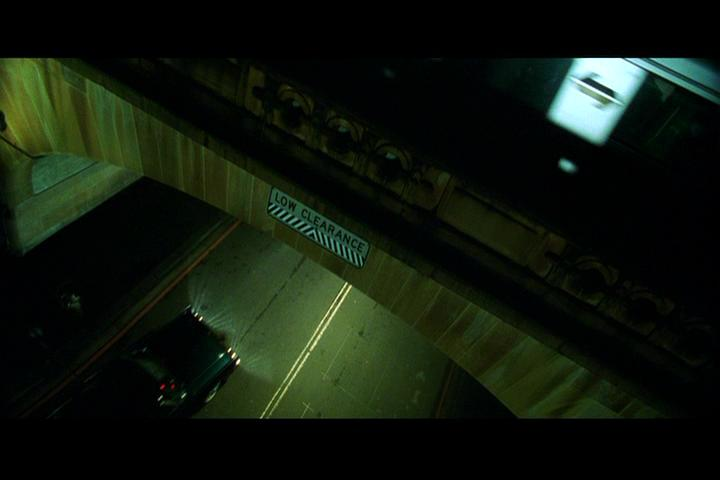
\includegraphics[width=0.5\linewidth]{fig/8b758b82f42f6090f603a6f5.jpg}
\end{figure}

接下来有一段Neo在Mobil Ave的镜头,就是Neo沿着铁轨跑,结果从另一面回来了。有人说那是搞笑,事实上,那也是很重要的,正是我说的轮回世界三个限制之一,空间。我说过导演经常在这几个方面作文章,关于“空间”的具体例子就是开锁匠的走廊,法国人的城堡,设计师的房间,火车人的车站。事实上,这里的奔跑正代表轮回(samsara)。其实“轮回”这个翻译并不佳,samsara还有“看不清真我,得不到梵,相信虚幻的世界”这些含义。不是“生,死,再生”可以涵盖的。

接下来,那个三人小组到了法国人的场子。

\begin{myquote}
Q-Ball Gang Member \#1: You've got to be kidding ...

Q-Ball Gang Member \#2: Holy shit, it's Wingless.

Q-Ball Gang Member \#1: I get it. You must be ready to die.

Seraph: I need to speak with him.

Q-Ball Gang Member \#1: The only way you're getting through this door is over my big dead ass.

Seraph: So be it.
\end{myquote}

够酷吧,Seraph一句“那好吧”真是够力度。其实,我们在这里也可以看出来Seraph和法国人是老相识了。

下面这张图也有些内容可以聊聊。首先这个拱形的入口代表性,第二部里Neo和Trinity在ML的时候,也是这个拱形结构。《达芬奇密码》里也指出过拱形和性的关系。左边的石座上有倒十字的标志,是反基督的一个标志。不要忘了,这里的主人Merovingian的名字来自法国六个封建王朝第一个,被认为是耶稣的后裔。这可不是《达芬奇密码》的原创,事实上,Merovingian家族被如此看待已经几个世纪了。而法国人这个地方就是个反基督的地方。叔本华说过:“然而一个像上帝如耶和华的神,由于纯粹的幻想而创造了这个苦难的世界,且乐此不疲,额手称庆,褒赞其成功,然后宣布凡物都是美好的——这真是行不通的事。”而尼采更是写了《反基督》这样的书。可笑的是基督徒还很支持《黑客帝国》里的圣经隐喻,却对《达芬奇密码》穷追猛打,由此我们也可以看到普通影迷看电影的本事到底如何了。

\begin{figure}[htb]
\centering
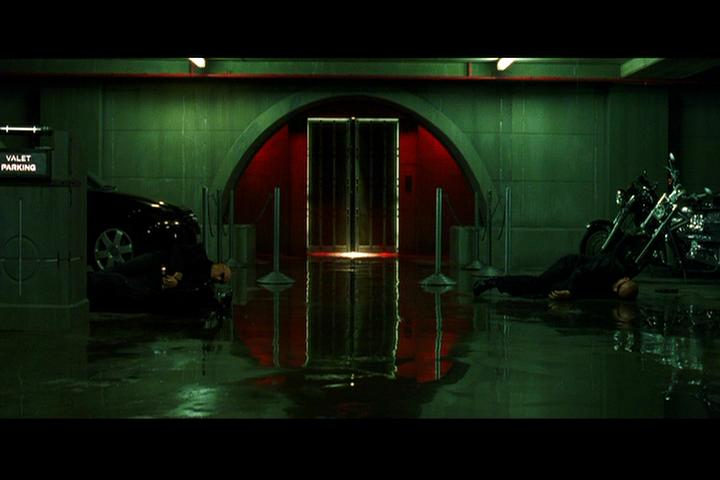
\includegraphics[width=0.5\linewidth]{fig/4fd64bed745da1d4b31cb1f5.jpg}
\end{figure}

接下来就是一段很有型的枪战,没有什么特别要讲的。提一下这里5个反派的名字,第一个被杀死的家伙叫Dogboy,两个长的挺像的光头,一个叫Rook,一个叫Pinball Wizard,被小崔踢进墙的家伙叫Jerry, 戴防毒面具的家伙姓名不详,演员的真名叫Alex Kuzelicki。

这些名字也是有意思的,Rook是小说《时间机器》里的一个科学家的名字,后来Warren Publishing公司出版的很多漫画中都出现他。Pinball Wizard原意是弹球游戏的终极关,导演指的是The Who乐队的一首60年代摇滚歌曲。而Dogboy就不好说了,是很常见的外号。而Jerry这个名字就是最重要的,《猫和老鼠》都知道吧,齐泽克曾经在解释大他者的时候用《猫和老鼠》举过例子,无论猫或是老鼠在哪一集被整的很惨,甚至升天了,都不影响在下一集里完好的出现。很奇怪的是,Tom猫才是老被整的对象,而齐泽克的具体例子里却偏偏说Jerry被整的一次(嘴里炸药爆炸,然后被切成片)。

下面这张图就是Jerry被Trinity袭击的画面。小崔这招牌踢又出现了。

\begin{figure}[htb]
\centering
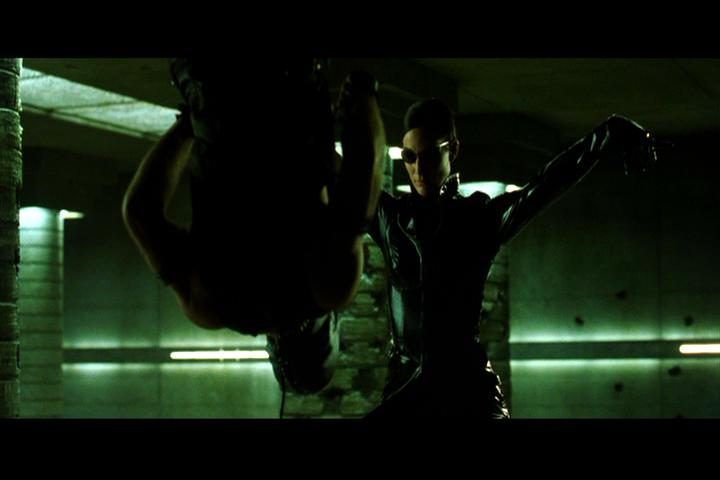
\includegraphics[width=0.5\linewidth]{fig/328dcf1b4553d7faaf5133cc.jpg}
\end{figure}

\begin{myquote}
Merovingian: What in the hell? *laughs* I don't believe this.

Merovingian: *to the DJ* Hey. Hey! *to Seraph* The prodigal child returns. L'ange sans ailes (Trans: The angel without wings). Are you here for the bounty, Seraph? *laughs heartily* Tell me, how many bullets are there in those guns? I don't know, but I don't think you have enough.
\end{myquote}

法国人这句“What in the hell”挺逗的,这里就是Hel嘛。这里可以看出来,Seraph以前是跟法国人的,后来先知成了系统最重要的部分,Seraph就保护先知了。另外,我们还可以看到Trinity爱情的盲目,Seraph本来建议回去问先知,小崔救夫心切,子弹都没带够就去法国人那里砸场子。

\begin{myquote}
Seraph: We only want to talk.

Merovingian: Oh, yes, I'm sure you do, you have fought through hell to do so, yes? I'll tell you what I'll do. Put down the guns and I will promise you safe passage out of here.

Seraph: All three of us.

Merovingian: Oh, yes, yes. Of course.
\end{myquote}

又是这句很阴险的“当然”,说明法国人要放他们出去是有目的的。别以为小崔手枪一顶,法国人就妥协了。我在本文开始就说过,法国人也是革命者,他代表的是废弃程序的利益。如果Matrix一再的循环,他永无出头之日。这时候他虽然控制了Neo,照理说循环已经被打破了,法国人可以肆无忌惮的增长势力,而不怕每次Matrix升级的时候,救世主都来砸场子。但事实并非如此,Neo还有个复数Smith呢,小史可比Neo难对付,法国人要是被Smith侵入了,唯一可以和他抗衡的Neo又被困在别的世界,那不就完蛋了嘛。他不直接放人,而和对现今形势一无所知的小崔他们讲条件,太奸商了。

\begin{myquote}
*Trinity, Seraph, and Morpheus put down the guns and are escorted up the stairs*
\end{myquote}

这里导演又拿基督教开涮了。二楼包厢的一个角落里,一个白衣MM手里端着一个巨大的苹果,分明是暗示夏娃用苹果引诱了亚当,结果下地狱了。图我就不截了,有心的朋友可以自己去看。

\begin{myquote}
Merovingian: *laughs* Quelle bonne surprise, n'est pas? (Trans: What a fine surprise, isn't it?) Who could've guessed we'd all be seeing each other so soon after our last meeting? A fate too kind. And since you, my little Judas, have brought them here, I can only surmise that the fortune teller has found herself another shell? Disappointing, but not unexpected. I do hope, however, she has the good manners to learn her lesson, and to remember that there is no action without consequence. And if you take something from me you will pay the price.
\end{myquote}

这里就开始讲他的工作原理了:consequence。这个词在逻辑学里也是因果的意思,也可以说是一系列的推论。另外提到“价值”,这是选择的重要指标(说唯一指标太绝对了),也是推论的一个重要方向。价值产生于欲望,“欲望来自我们对未来的思考”(叔本华语),法国人就是以当前的情况来推论过去的价值。但“时间这一主动力使每一刻变得毫无价值”(叔本华语),所以法国人就没用了。(这一点是形而上学的,并不是说法国人在实际中没有用,导演这么安排是为了突显这种哲学理论)

\begin{myquote}
Seraph: You know why we are here.

Merovingian: *laughs* Come, now. What kind of question is this? Of course I know. It's my business to know. Some might think this a strange coincidence, but I do not. I am curious, though, as to how it actually happened. Do you know?
\end{myquote}

这里就可以看到各种人和程序对自己的目的和命运的态度。

Morpheus:fate

先知:purpose

Smith:not free

开锁匠:meant

Rama:karma

法国人:business

法国人是利用他的目的在为自己获得利益,是最实在的一种方法,比起Rama的“感激命运”实惠多了。另外注意法国人问的这个问题:“你认为这是怎么发生的?”他问的是现在的处境是如何造成的,答案就是Neo他们砸他场子,带走开锁匠,杀死他大量手下,法国人囚禁Neo是在报仇。

\begin{myquote}
Trinity: No.

Merovingian: No? I didn't think so. But it is always best to ask.

Morpheus: We want to make a deal.

Merovingian: *laughs* Always straight to business, huh, Morpheus? Okay. I have something you want. To make a deal, you must have something I want, yes? And it so happens there is something I want. Something I've wanted ever since I first came here. It is said they cannot be taken, they can only be given.
\end{myquote}

这就是我说的奸商部分,自己分明就要放人的,还要敲诈一笔。

\begin{myquote}
Morpheus: What?

Merovingian: The eyes of the Oracle. *laughs*

Merovingian: I have told you before, there's no escaping the nature of the universe. It is that nature that has again brought you to me. Where some see coincidence, I see consequence. Where others see chance, I see cost. Bring me the eyes of the Oracle, and I will give you back your saviour. That seems a particularly fair and reasonable deal to me. Yes, no?
\end{myquote}

我曾经开过一个玩笑,说Eye(i)是-1的平方根,Smith是Neo的复数,也就是-1。先知的眼睛把Smith给开了方,Smith就成无理数了。言归正传,先知的眼睛象征先知的能力,最终也确实是先知的能力害Smith被毁。

“先知的眼睛”这个意象出自普希金的一首诗《先知》(六翼天使Seraph也在其中出现):

{\centering \it

忍受着精神上的煎熬,

我缓缓地走在阴暗的荒原,

这时在一个十字路口,

六翼天使出现在我的面前。

他用轻得像梦似的手指

在我的眼珠上点了一点,

于是像受了惊的苍鹰,

我张开了先知的眼睛。

他又轻摸了一下我的耳朵,

它立刻充满了声响和轰鸣:

我听到了天宇的颤抖,

天使们翩然在高空飞翔,

海底的蛟龙在水下潜行;

幽谷中的藤蔓在簌簌地生长。

他附身贴近我的嘴巴,

一下拔掉我罪恶的舌头,

叫我再也不能空谈和欺诈,

然后他用血淋淋的右手,

伸进我屏息不动的口腔,

给我安上智慧之蛇的信子。

他又用利剑剖开我的胸膛,

挖出了我那颤抖的心脏,

然后把一块熊熊燃烧的赤炭

填入我已经打开的胸腔。

我像一具死尸躺在荒原,

上帝的声音向着我召唤:

“起来吧,先知,你听,你看;

按照我的意志行事吧,

把海洋和大地统统走遍,

用我的语言把人心点燃。”

}

另外,这里法国人的一句“别人看到巧合,我看到因果;别人看到机会,我看到代价”也是经典,这就是几率论者和全定论者的区别。这里我要举一个对于“完事无因”的著名反驳:“完事无因”这句话要么有原因,要么没有。如果这句话没有原因,那就没法证实它是对的;如果这句话有原因,本身就证明了原因的存在。

\begin{myquote}
Trinity: I don't have time for this shit.

*Hel Club upstairs fight*

Trinity: You want to make a deal, how about this? You give me Neo, or we all die right here, right now.

Merovingian: Interesting deal. You are really ready to die for this man?

Trinity: *cocks gun* Believe it.

Perseph: She'll do it. If she has to, she'll kill every one of us. She's in love.

Merovingian: It is remarkable how similar the pattern of love is to the pattern of insanity.

Trinity: Time's up. What's it gonna be, Merv?
\end{myquote}

“爱”和“疯狂”多么相似啊!难怪很多哲学家都标榜只有性,没有爱。叔本华、尼采都是如此,弗洛伊德就不说了,分明是个“淫秽的哲学家”,当今的肯韦伯几乎做了和尚,齐泽克经常讲黄色笑话,就是对“爱情”绝口不提。

这一部分开始前,先告诉大家一个好消息,neverwin已经结束了第二部的非官方解释,相信这两天就会开始写neverwin版的第三部非官方解释了!(neverwin达人看到的话,别忘了给小弟“杂物”的版本也做做广告哦,哈哈)

\begin{myquote}
Neo: Ok. You got yourself into this. You can get yourself out.
\end{myquote}

这里Neo预见到了他最后要走的路。这是一个突破,因为这一次是Neo尽力去感知的,而不是像以前那样灵光一闪。按黑格尔的说法,Neo正在努力看透一切。而这个地方正是轮回的表现,看透轮回就可逃出这个地方,结果下一个镜头火车就到了。我们当然知道这是Trinity拼命做到的,但我们也要理解导演要求如此拍摄和剪接的意思。

这火车也很有意思,火车人在被Seraph他们追得跳火车的时候,我们可以看到这些火车前都有Loop(环形线)的字样,而这辆车进站的时候,我们可以看到那个位置被挖空了,说明循环被打破。但Matrix一样是轮回世界,连Zion都是一样。但虚拟派不要抓着我这句话说Zion也是虚拟的。无论你信不信先知,她一样可以利用你,无论世界是否虚拟,你永远受着控制。(相对叔本华的终极自由而言)

\begin{figure}[htb]
\centering
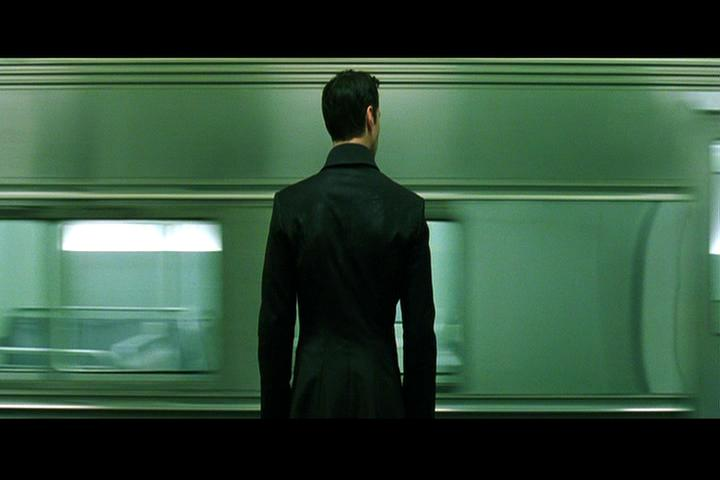
\includegraphics[width=0.5\linewidth]{fig/926a29387d14c524b8998fe3.jpg}
\end{figure}

\myparsep

\begin{myquote}
Morpheus: Are you ready for us?

Link: Almost, sir. They got some pretty ancient hacks here, we're working on it. Did you find Neo?

Morpheus: Can't you see him?

Link: No, sir. We were reading something but I couldn't tell what it was.

Neo: I can't leave yet.

*Trinity looks over at him*

Neo: I have to see her.

Trinity: Now?

Neo: This is my last chance.
\end{myquote}

这里可以解决一个关于Bane被入侵时未被发现的问题。neverwin的解释是Bane醒来说自己逃出来了,船员也会相信的。其实在这里可以看出来,船员们根本没有看到Bane被Smith入侵。黑迷们还记得Logos启动之后Sparks的反应吧,他说Matrix的信号有问题。当时Matrix不稳定的原因只有一个,那就是Smith的蔓延。所以说Bane被入侵的时候,船员们根本无法从屏幕中读出什么来。况且看数码雨是要经验的,头一回看到这样的事情,即便屏幕清清楚楚,他们也未必知道到底发生了什么。

这段和第一部里几乎一模一样,唯一不同的是开车的人变了,第一部是Cypher开的车,这里是Seraph,而这两个家伙都是“叛徒”。区别是Cypher“变坏”,Seraph“变好”。

\begin{figure}[htb]
\centering
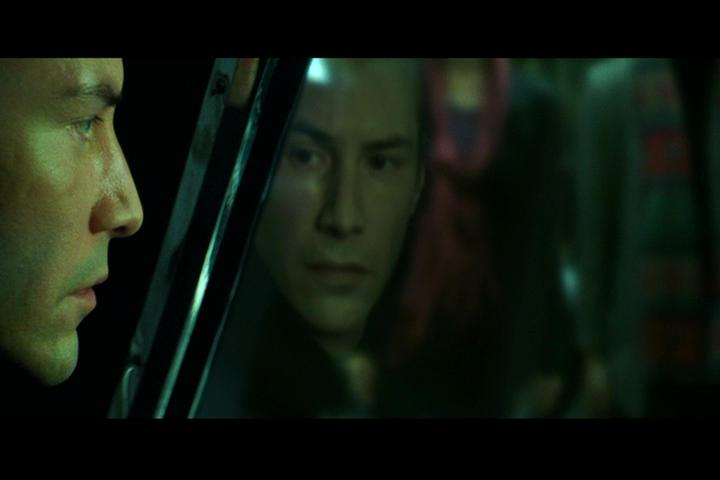
\includegraphics[width=0.5\linewidth]{fig/f64563d08227bd8fa0ec9ce3.jpg}
\end{figure}

到先知那里了。

\begin{myquote}
Oracle: That's it. That's the secret. You've got to use your hands.

Sati: Why?

Oracle: Cookies need love like everything does.
\end{myquote}

饼干也需要爱!先知开始教Sati那些人类的情感。先知教的这种爱是博爱,这一点叔本华是很缺乏的。但奇怪的是佛教很讲究博爱,而叔本华又研究多年佛学,他怎么就那么悲观呢?看来,Neo和Smith正是叔本华的两面,也是导演的两面,也是我的两面。任何一个既欣赏叔本华,又敬重佛教的人都会有这样的情况。

\begin{myquote}
Sati: Neo!

Oracle: I was hoping to have these done before you got here. Oh, well. Sati, honey, I think it's time for a tasting. Take the bowl to Seraph and find out if they're ready.
\end{myquote}

又一次证明先知的能力是“直觉”,Neo什么时候来这样物理因素很重的事件是很难预测的,但是先知确实预测到了Neo会来。

\begin{myquote}
Sati: Okay. *to Neo* I'm glad you got out.

Neo: Me too.

Oracle: So, do you recognize me?

Neo: A part of you.

Oracle: Yeah, that's how it works. Some bits you lose, some bits you keep. I don't yet recognize my face in the mirror, but ... I still love candy. *offers Neo a piece of red candy*
\end{myquote}

很精辟,佛经上讲:“得就是失,失就是得,有得必有失,有失必有得。”同一件事情的得与失比例对于不同的人来说是不一样的,你若能平心看到“得等于失”,那你就得道了。

\begin{myquote}
Neo: No, thank you.

Oracle: Remember what you were like when you first walked through my door, jittery as a junebug? And now just look at you. You sure did surprise me, Neo, and you still do.
\end{myquote}

哈哈,Smith说伟大的先知绝无意外,而先知自己却说Neo给了她很多惊喜,说明先知对Neo的直觉并不永远准确。还好,这一点并不会对大问题产生影响。

\begin{myquote}
Neo: You gave me a few surprises, too.

Oracle: I hope I helped.

Neo: You helped me to get here, but my question is why? Where does this go? Where does it end?
\end{myquote}

救世主问原因了,这是Neo在法国人那里学来的(第二部里,法国人就给他灌输这种思想),原因是动力啊。叔本华认为一个人的行为有两个因素:动机和性格。原因就是动机,这是没有争议的,而性格,既然是塑造出来的,同样也可以被改变。导演为什么在力求和第一部对应的时候安排先知提Neo的改变呢?就是要告诉观众,先知不旦给了Neo动机,甚至改变了Neo的性格。但不知有多少人理解导演的苦心。

\begin{myquote}
Oracle: I don't know.

Neo: You don't know or you won't tell me?

Oracle: I told you before. No one can see beyond a choice they don't understand, and I mean no one.
\end{myquote}

“没有人可以理解自己看不透的选择”,这没有什么需要解释的。需要解释的是“先知还有不理解的选择?”回忆先知之前和Morpheus、Trinity的谈话,先知明确知道她这个选择的代价,但最后这个选择的代价却比她预期的高,说明这是个错误的选择(仅仅就利益而言),那么就无法看透这个选择了。但这个利益上的错误选择却并不完全错误,利益的根本就是生存的欲望,而叔本华在《论自杀》中就说过,像是主义、信仰,就可以超越生死,何况仅仅是被Smith入侵呢。

\begin{myquote}
Neo: What choice?

Oracle: It doesn't matter. It's my choice. I have mine to make, same as you have yours.

Neo: Does that include what things to tell me and what not to tell me?

Oracle: Of course not.

Neo: Then why didn't you tell me about the Architect? Why didn't you tell me about Zion, the Ones before me --- why didn't you tell me the truth?

Oracle: Because it wasn't time for you to know.

Neo: Who decided it wasn't time?

Oracle: You know who. *She points at the Temet Nosce sign above the door*

Neo: I did. *Oracle nods* Then I think it's time for me to know a few more things.

Oracle: So do I.

Neo: Tell me how I separated my mind from my body without jacking in. Tell me how I stopped four sentinels by thinking it. Tell me just what the hell is happening to me.

Oracle: The power of the One extends beyond this world. It reaches from here all the way back to where it came from.

Neo: Where?

Oracle: The Source. That's what you felt when you touched those Sentinels. But you weren't ready for it. You should be dead, but apparently you weren't ready for that, either.
\end{myquote}

救世主的力量当然不能局限于Matrix,在任何一个世界都不应该被终结。而Neo那些问题可以很容易从无线接入来解释。关于Source的问题,先知说Neo在碰到乌贼的时候,就感知到了Source。事实上,那些乌贼就是Source,那就是本质。我们的思想不应该被局限于“Source是一个地方”,Source完全可以是一种精神、一种本质、一种灵魂。乌贼作为一种很基本的机器,就是很本质的。先知说Neo还没有准备好接受,那是当然的了,谁能接受自己的敌人居然如此高尚,如此纯洁?(这么说可能很多人摸不找头脑,看Neo眼瞎之后的视野就知道我在说什么了)

死不死的问题也很有趣:“你应该死了,但是还有准备好。”够绝!敢情不准备好死还死不了。Neo是否该死的问题没有必要解释,也无法解释,因为每个人(包括不用脑子看电影的)都明白,Neo死不了。

\begin{myquote}
Neo: The Architect told me that if I didn't return to the Source, Zion would be destroyed by midnight tonight.

Oracle: *rolls eyes* Please ... You and I may not be able to see beyond our own choices, but that man can't see past any choices.

Neo: Why not?

Oracle: He doesn't understand them --- he can't. To him they are variables in an equation. One at a time each variable must be solved and countered. That's his purpose: to balance an equation.

Neo: What's your purpose?

Oracle: To unbalance it.

Neo: Why? What do you want?

Oracle: I want the same thing you want, Neo. And I am willing to go as far as you are to get it.

Neo: The end of the war. *Oracle nods* Is it going to end?
\end{myquote}

看到了吧,先知要的也是和平。很多人以小人之心度君子之腹,说先知不过是为了一次完备的升级。人家先知是很……的!(没词了)这也符合在她公寓墙上找到的“peace”涂鸦。

\begin{myquote}
Oracle: One way, or another.

Neo: Can Zion be saved?

Oracle: I'm sorry, I don't have the answer to that question, but if there's an answer, there's only one place you're going to find it.

Neo: Where?

Oracle: You know where. And if you can't find the answer, then I'm afraid there may be no tomorrow for any of us.

Neo: What does that mean?

Oracle: Everything that has a beginning has an end. I see the end coming. I see the darkness spreading. I see death. And you are all that stands in his way.

Neo: Smith.

Oracle: *nods* Very soon he's going to have the power to destroy this world, but I believe he won't stop there; he can't. He won't stop until there's nothing left at all.

Neo: What is he?

Oracle: He is you. Your opposite, your negative, the result of the equation trying to balance itself out.
\end{myquote}

我们说过,Neo是逻辑外真理,是在等式之外的,Smith却是因为等式为了平衡而被建造出来的。解释就是先知硬是把逻辑外真理由值转为关系,借设计师的手创造了Smith这个可怕的负数。(我为什么在这里用“可怕”形容Smith呢?我和他有一样的哲学啊!)

\begin{myquote}
Neo: What if I can't stop him?

Oracle: One way or another, Neo, this war is going to end. Tonight, the future of both worlds will be in your hands ... or in his.
\end{myquote}

\myparsep

刚提到Smith,他就醒了。接下来的镜头Neo也醒了。可以看出两个人之间的联系。确实,我每次想到Smith那种理论,就要Neo似的问一句:“没有意义就不能坚持吗?”两者是共存的。

\begin{figure}[htb]
\centering
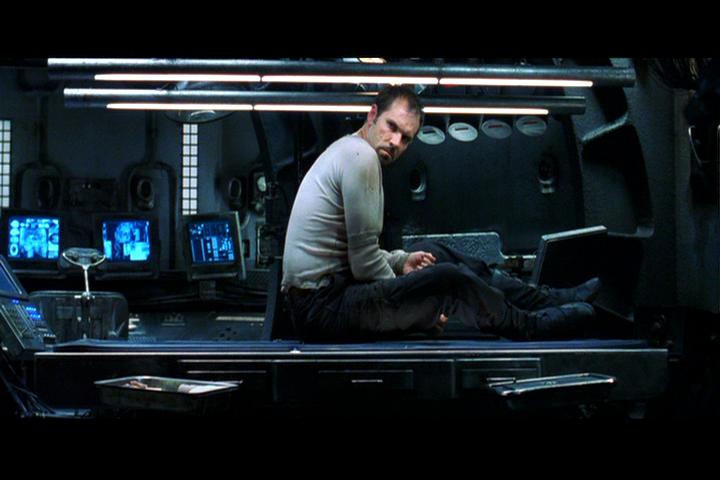
\includegraphics[width=0.5\linewidth]{fig/04eda1ec7ef97f3d26979102.jpg}
\end{figure}

\begin{myquote}
Trinity: How are you feeling? Are you all right?

Neo: I need time.

Roland: That figures.

Maggie: Captain Roland!

Roland: What's up, Maggie?

Maggie: Bane, sir. he's conscious.

Roland: Good. Maybe he's got some answers.
\end{myquote}

有意思,Roland还真有点直觉。Neo出来说“需要时间”,Roland就说“That figures”,人家这个船长不是白当的。先知理解人类的心理,Roland也不差。

现在回到先知那里,我们亲爱的Smith终于要出场了。

\begin{myquote}
Oracle: Mmm, I love that smell. I sure am gonna miss it.

Seraph: Oracle.

Oracle: I know, I know. Sati, honey! Take a few cookies and go with Seraph.

Sati: Can I come back? I would like to come back!

Oracle: I would like that too.

Sati: So I'll see you tomorrow.

Oracle: I hope so, honey, I hope so.
\end{myquote}

先知知道吃不上这饼干了,她烤这些饼干就是为了让Smith打翻的。有人会觉得这不是太无聊了吗?但是对先知来说,基本上一切都是已知的,她本来就是很无聊的程序。还有她们这里说的“明天”既是字面上的意思,又代表“未来”。先知的“hope”也是区分信仰者和非信仰者的重要标志。哈曼议员在最紧急的关头说他们还可以“希望”,而Lock指挥官就明确地说:“希望是不合时宜的奢侈。”

下面一张图也很有意思,先知给了Sati一些饼干,但却不是刚刚烤好的那些。呵呵,饼干都是有目的的。给Sati的饼干就是让她吃的,刚烤好的就是给Smith打翻的。

\begin{figure}[htb]
\centering
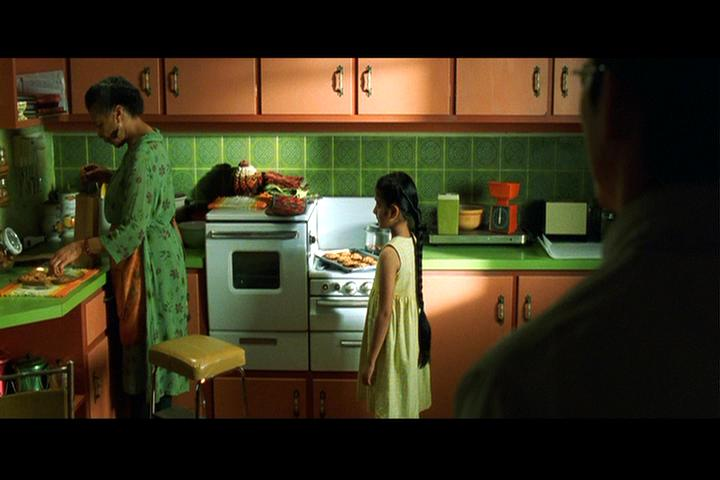
\includegraphics[width=0.5\linewidth]{fig/42486159b22efa2a2834f002.jpg}
\end{figure}

Seraph带Sati走电梯,电梯却坏了。这个neverwin解释的很清楚,《黑客帝国》里的电梯只能上,不能下。他们回头看走廊,灯一盏接一盏灭了,而墙上又出现那个的标志。先知说的darkness spreading就是指Smith,那个标志当然也是指Smith,难怪Hugo Weaving是V字仇杀队主演的最佳人选。

\begin{figure}[htb]
\centering
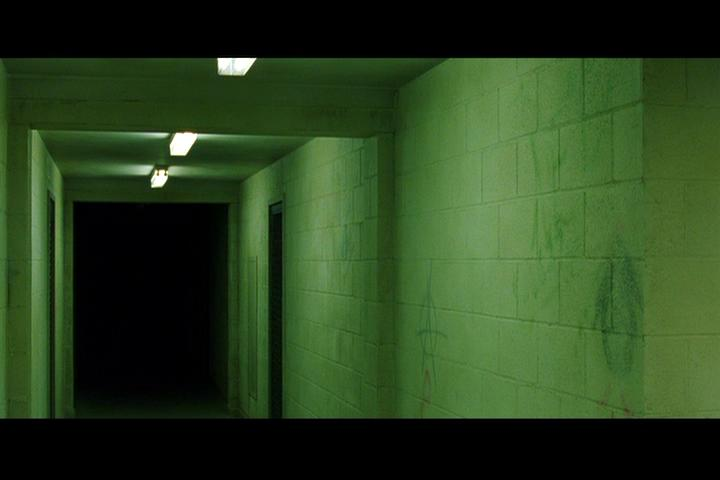
\includegraphics[width=0.5\linewidth]{fig/c621faf21812bd13b07ec502.jpg}
\end{figure}

\begin{myquote}
Sati: I'm scared, Seraph.

Seraph: Come.

Sati: He's following us.

Smith: Well, well, it's been a long time. I remember chasing you was like chasing a ghost.

Seraph: I have beaten you before.

Smith: That's true, but as you can see, things are a little different now. *to Sati* And you must be the last exile.

Sati: The Oracle told me about you.

Smith: Really? And what did she say about me?

Sati: That you're a bad man.

Smith: Oh, I'm not so bad once you get to know me.
\end{myquote}

“先知说你是坏人。”

“你了解我就不觉得我很坏了。”

就是嘛!真正了解Smith不但觉得他做的事无可厚非,而且他还很可怜。叔本华过“当作为世界主宰的意志以个人的形式出现时,就会引起我们的同情,常觉得它所获得的是多么的少,以致只能维持其自身的肉体,这也就是人类会如此悲惨的缘故。”一旦Smith控制了全世界,那他就可怜到只能维持自己。

审问Bane这一段。

\begin{myquote}
Bane: I really wish I could help, but I just ... I don't remember any of it.

Roland: What about the cuts on your arms? Those cuts are more than one day old.

Bane: Yeah, definitely. You're right about that, sir. They look like they might be self-inflicted. Why would I do something like that to myself? Unless, of course, I wasn't myself ... but ... if I'm not me, then who am I?
\end{myquote}

“我是谁?”我既不是Bane也不是Smith,因为无论是Bane还是Smith,都来自别人的认知,和自己对自己的认识肯定是不一样的。只有在一种情况下,“我是谁”才有标准答案,那就是每个人都是Smith,这也正是Smith要做的事情。

\begin{myquote}
Roland: Has this man been tested for VDTs?

Maggie: Yes, sir, it was negative. But he is showing a lot of unusual neural activity. Some cross-synaptic firing as well as signs of recent trauma, with fresh fibrotic scarring throughout the cortex.
\end{myquote}

交叉神经焦灼,近期外伤,脑皮层遍布纤维疤痕。

仔细想一想,这个交叉神经焦灼和外伤不是把原本的思维方式给完全破坏了吗?而新生成的纤维质就像宽带代替了电话线一样,代替了神经,Smith把自己的数据导入那些纤维,那他就是Smith了。这时的Bane就像一个瓶子,装水就是水瓶,放花就是花瓶。

需要注意的是,这并不是生物入侵,而仍然是数据入侵,Smith只是用控制RSI(就是Matrix中的自我形象)的方式控制真实的肉体。

那么请问Smith如何通过Matrix完成如此复杂的“手术”?相比之下不如解释成Smith通过某种催眠或洗脑的方式使得Bane以为自己是Smith,并继承了Smith的记忆。

交叉神经焦灼、大脑纤维化,这都是电影中说的,没有必要去找其他的解释。况且这个“手术”并不复杂,烧坏脑子、纤维化都是Cyberpunk作品中经常提到的副作用,第一位脑部和电脑连接的科学家Kevin Warwick在他的书中就指出过这种副作用的可能性。另外,他还为黑客帝国写了一篇名为The Matrix --- Our Future的文章。

\begin{myquote}
Bane: What's that for?

Maggie: To help you relax. To make it easier for you to remember.

Bane: What if I don't want to remember?

Maggie: Why would you want that?

Bane: What if I blew that EMP? What if I did destroy those ships and I am responsible for the deaths of all those men? If I did that, it wouldn't be very safe for me here, would it?

*Maggie tries to inject Bane with the relaxant, but he stabs her and she falls over dead*

Bane: Of course, it might not be very safe for you, either.
\end{myquote}

如果我不想记得呢?这是个好问题啊!虽然Smith这是在演戏,是在演Bane,但是说的道理很经典。我之前说过导演俩很喜欢《1984》,在那本小说里有这么一段(记不太清了,可能有出入),是温斯顿和奥勃良在聊天。他们说过去并不存在,过去是被记录下来的,如果他们破坏掉所有过去的记录,并且造出自己的,那他们就改变了过去。

这就是说,你不知道过去,那过去对你来说就不存在;如果你是唯一一个知道这段过去的,你一忘,那这一段过去对任何人来说都不存在了。当然,在影片这一段里,这个过去并非不为人知,人人都知道飞船被毁了,船员都被杀了,但是这个事件的细节确实只存在Smith一个人心中。其实在第一部中也有这个体现,Cypher和Smith的交易中就有一条“忘记过去的一切”。

莱布尼兹对于身心间的因果关系可以很好解释这个问题。Hopkins大学的Sean Greenberg教授有一篇研究《黑客帝国》中莱布尼兹哲学的文章,就放在黑客帝国的官方网站上,我们可以按照他的思路接着讲。莱布尼兹认为身心间的因果是个幻觉,是无窗单子的状态改变造成的。因为单子间没有关系,是完全隔绝的,造成了因果关系的是单子间意外的和谐,这样来讲,被遗忘的过去不再和其他单子和谐共存,于是就被从因果关系中剔除了。

\begin{myquote}
Smith: The great and powerful Oracle. We meet at last. I suppose you've been expecting me, right? The all-knowing Oracle is never surprised. How can she be, she knows everything. But If that's true, then why is she here? If she knew I was coming, why didn't she leave? *sweeps plate of cookies off table* Maybe you knew I was going to do that, maybe you didn't. If you did, that means you baked those cookies and set that plate right there deliberately, purposefully. Which means you're sitting there also deliberately, purposefully.

Oracle: What did you do with Sati?

Smith/Sati: Cookies need love like everything does.

Smiths: *laugh*

Oracle: You are a bastard.

Smith: You would know, Mom.

Oracle: Do what you're here to do.

Smith: Yes, ma'am.

Smith/Oracle: *laughs maniacally*
\end{myquote}

很多人觉得先知并不能预测Smith要打翻饼干,但那无法解释先知烤好饼干说的“可惜我吃不上了”。知道自己吃不上了还烤,那当然是预知到了Smith的做法,而且是要成全这个举动。这和让Neo打碎花瓶一样,先知知道对Neo说那一句话,Neo就会转身,所以她把花瓶放在了大门边(第三部里花瓶不必被打碎了,就放远了)。这里先知同样知道Smith会把面前的东西打碎,所以就把饼干放在了Smith的面前。先知要是把自己的烟灰缸放在那里,Smith就会打碎烟灰缸了。这里还有个小细节,Neo到这里来的时候,桌子上放着很多东西,这时候全都清走了,就是为了Smith注意饼干。东西全放在那里的话,就不清楚Smith会打翻什么东西了。打翻饼干其实也是个隐喻,这饼干是用“爱”做的,Smith的所做所为就很好理解了。

Smith说“饼干也需要爱”之后那诡异的笑不只是向先知说“Sati也被我入侵了”,他同时也是在嘲笑这句话本身。Smith不明白爱,他只有恨,而且并不是“博恨”(造词了),他只恨Neo。Seraph也打败过他,但他并不恨Seraph, 他是很有原则的。所以说Smith并不坏,正如他自己说的那样,只是他的世界观不被接受而已。

这里Smith管先知叫妈妈,没有什么需要具体解释的,我们知道Smith就是先知造成的。通常认为Smith是Neo和机器大帝谈判的筹码(没有错,但不完全),Neo和Smith既然是正负的关系,无论是否以这种方式终结,他们始终是要终结的。Neo不存在了,机器也没法建立下一代Matrix,那就没有救世主把最初的那些人救出去。毁掉Zion就意味着Matrix中百分之一不稳定的人会留在系统里,这是机器不希望发生的(除非它们真的像设计师说的那样准备接受另一种生存)。Neo的谈判只是暂时达到和平(不毁掉Zion不代表不攻击人类)。

还有Smith最后的大笑,前些天有人提问Smith是在笑什么。我们应该记得Bane的一段台词,Bane/Smith拿枪对着Neo的时候,问他还记得这个场面吗,他自己说“Think of nothing else”。既然他一直在想报复Neo,获得先知能力之后第一件事就是看Neo的未来。我们应该还记得Neo躺在大坑里,Smith说他看到这个场景了,这就是end,说明Smith在这时看到的就是自己打败了Neo,当然高兴得大笑。其实先知也只能看到这里,先知在前面说“没有人能看透自己不理解的选择”,她也只看到了Neo被Smith打倒在地,所以她只能believe那个未来。

\begin{figure}[htb]
\centering
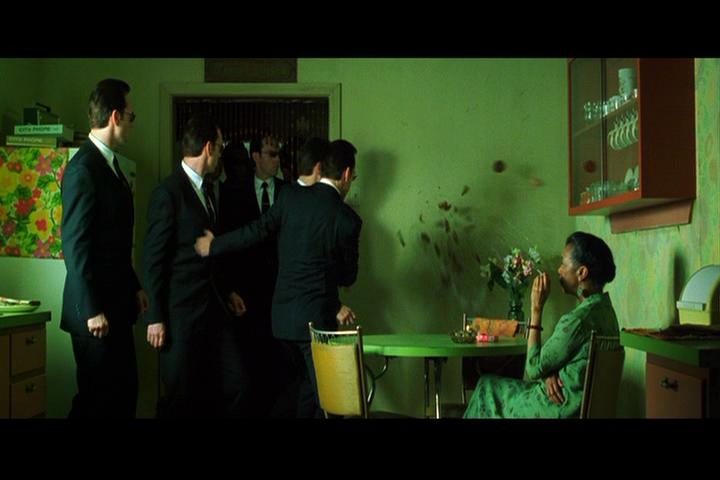
\includegraphics[width=0.5\linewidth]{fig/45c00df489aee5ef7609d702.jpg}
\end{figure}

\myparsep

\begin{myquote}
Roland: I want the truth. I don't care what it takes. Make him remember.

Mauser: Sir? We found her!

Roland: The Logos?

Mauser: Yes, sir.

Roland: 'Bout time we had some God damn good news.

Morpheus: Are the thermals picking up any signs of life?

AK: No, sir. Nothing yet.

Roland: What about the ship?

AK: Well, holographic says the hull is still intact.

Roland: Drop her down [...]

Colt: Yes, sir.

Roland: Get a full diagnostic on that ship as fast as humanly possible.
\end{myquote}

这里Roland在说“好消息”的时候又用了God damn一词,就是说这个“好消息”也是注定的。这里挺有意思的是,老莫很着急地问“有生命信号吗?”听到否定的回答,就一脸伤心样。当然了,他担心的是Niobe。至于Ghost和Sparks, 老莫只会来一句“他们都是好同志”。

\begin{myquote}
Colt: Careful, sir! The squids are sneaky bastards. Could be a trap.

AK: What was that?

Niobe: You can put that shit away, boys. All she needs is a jump.

Morpheus: Niobe.

Niobe: Morpheus. Are you all right?

Morpheus: Yes, I'm fine. We didn't know what happened after. I'm sorry.

Niobe: It's okay. I'm happy to see you too. Did you get Neo out?

Morpheus: Yes. How did you know about that?

Niobe: The Oracle.

Morpheus: You saw her?

Niobe: Just before the sentinels found us.

Morpheus: What did she tell you?

Niobe: The same thing she always does. Exactly what I needed to hear.
\end{myquote}

先知总对Niobe说的就是那句“你自己拿主意”。Niobe说这是自己正想听的,正好突出Niobe果断的性格。Don Davis为Niobe开飞船所做的配乐名叫Die Brünett Walküre,是德文的,这个名字来自尼采最喜欢的一位德国作曲家瓦格纳的作品,Der Ring des Nibelungen(尼伯龙根的指环),其中第二部分就叫做Die Walküre(女武神)。而Brünett意思是棕色头发,Niobe就是棕色头发的女武神。

\begin{myquote}
Lock: In less than 12 hours, the machines will breach the dock walls. Every simulation we've run, we've seen that once the machines are inside the city, the odds of our survival decrease dramatically. Thus our primary objective must be to destroy or disable the diggers inside the dock. If we can do that, perhaps we can prevent them from ever reaching the city. If not, the only place we'll be able to mount an effective defense will be at the entrance of the Temple. It is small enough that it will force them into a bottleneck, allowing us to concentrate the remainder of our defense.

Councillor Dillard: We understand that you've requested additional volunteers.

Lock: That is correct.

Councillor West: Precisely what size of force are you planning to commit to the primary dock objective?

Lock: Right now, the entire APU core and half the infantry.

Councillor West: Half the infantry?

Lock: If it were up to me, Councillor, I'd take every man, woman, and child, put a gun in their hands and march them straight into that dock.

Councillor Dillard: Perhaps it is best that it is not up to you.

Lock: Time will tell, Councillor.

Councillor Hamann: Commander, just one more question. Has there been word from the Nebuchadnezzar?

Lock: None, and at this point there's no reason to expect that there ever will be.

Councillor Hamann: Perhaps. But we can hope.

Lock: I'm afraid hope is an indulgence I don't have time for.
\end{myquote}

黑客帝国的思想分为三部分,Zion是身体,Matrix是思想,Machine是灵魂。在真实世界很少有很高深的内容,就解释一下这些人名字的含义吧。

议会成员:

Councillor Hamann指的是Johann Georg Hamann,是个德国哲学家,也是康德的好朋友。齐泽克就曾指出导演兄弟一定非常了解康德。虽然导演也很了解哈曼,但是并不相信他的很多东西。有趣的是,康德影响了叔本华,哈曼影响了黑格尔,叔本华和黑格尔却又是死对头,站在叔本华这边的导演当然不会过多地加入哈曼的东西。比如他在第二部和Neo讨论什么是控制的时候,只涉及了“定义”的问题,这类似黑格尔的感性确定性,是很小一部分导演认为黑格尔说对的东西。

Councillor Dillard指的是作家Annie Dillard,她曾获1975年的普利策奖。导演用这个名字就是因为喜欢她的诗歌而已。既然不是哲学家,我也就没什么说的了。

Councillor West指的是哲学家Cornel West,他的扮演者就是Cornel West本人。他是导演的私人朋友,但在电影里并没有明确指出他的理论,那说一些有趣的事吧。这个家伙在做黑客帝国评论音轨的时候老是抢着说话,我记得郭大路兄的《终结套装观碟笔记》里说他对东方哲学还有佛学很有研究。这就是我觉得他有意思的地方,因为和他一起做音轨的“心理学的爱因斯坦”Ken Wilber更厉害,Ken曾经在西藏跟六个大仁波切学禅,比West正规得多,而West却总是抢着说佛教方面的东西。

\begin{myquote}
Cas: Zee, what are you doing?

Zee: Making shells.

Cas: They're evacuating our level. We have to go.

Zee: I'm not going with you.

Cas: What?

Zee: They've called for volunteers to hold the dock.

Cas: *to the kids* Kids, you stay here. *to Zee* I know how you feel, Zee, but you can't do that.

Zee: I have to.

Cas: Why?

Zee: Because I love him. I love him the same as he loves me. And if I were out there and he were here, I know [what he'd do].

Cas: But you're gonna get yourself killed. It's crazy, Zee.

Zee: Maybe it is. But ask yourself, if it were Dozer, and you knew the only chance you had to see him again was to hold the dock, what would you do?

Cas: Make shells.
\end{myquote}

简单的对话,无非是表现“爱”这个大多数哲学家不以为然的东西,但用在这里却挺合适的。Matrix里的人都是深沉的、哲学的,Zion里的人都是热情的、情绪化的。所以说,写到这里就是我最头痛的部分了。

\begin{myquote}
Mifune: What the shit is going on over here?

Kid: An accident, sir! I didn't see ... I'm sorry!

Mifune: Who the hell are you?

Kid: I'm here to volunteer, sir.

Mifune: What's a pod-born pencil-neck like you doin' volunteering for my corps?

Kid: I want to do my part, sir! We gotta hold the dock.

Mifune: How old are you, kid?

Kid: Eighteen.

Mifune: Shoulda said sixteen, I mighta believed that!

Kid: OK, I'm sixteen.

Mifune: Minimal age for the corps is eighteen. Sixteen's too young!

Kid: The machines won't care how old I am. They'll kill me just the same.

Mifune: Ain't that the god damned truth?

Kid: Give me a chance, sir. I won't let you down.

Mifune: You do ... you'll find me and the machines have something in common.
\end{myquote}

解释一下Kid的名字,他其实就是黑客帝国动画版中Kid's Story中的那个小子。他在Matrix中的名字是Michael Karl Popper,暗指一个奥地利哲学家Karl Raimund Popper。他最著名的理论就是对观测归纳法的批判,Kid正是通过质疑观测归纳法脱离Matrix的。而那个名字Michael就不确定了,一来导演俩是乔丹迷,可能用了他的名字;二来也可能指炽天使米迦勒(St. Michael)。我个人倾向于米迦勒的解释,因为导演在解释Morpheus眼镜反射Neo选药片的镜头时说过,右边镜片里是Neo和红药片,左边的代表Anderson先生和蓝药片。那么说明导演为这个Kid也准备了两种身份,Matrix中那个应该对应米迦勒的反面,熟悉圣经的朋友应该知道,米迦勒的双胞胎兄弟就是堕天使Satan,而Kid也正是从楼上跳下来摔死的。另外,TomCatMao兄指出过Kid在学校的Locker上画着一条向下冲的龙,代表Kid将跳楼而死。而Satan堕天的时候正是以龙型降世,尾巴扫下天上三分之一的星。

\begin{myquote}
Ghost (v. o.): Okay. Charge the igniter.

Sparks: She lives again.

AK: You want us to patch an uplink to reload the operations software, Sparky?

Sparks: Yeah, that'd be swell. You can clean the windshield while you're at it. Uplinks are in place. I'm bringing her back online. Looking good, except, uh ... something wrong with the Matrix feed.

AK: No, there's not. You're looking at what we're looking at.

Sparks (v. o.): What the hell's going on in there?

Link: Whatever it is, it can't be good.
\end{myquote}

这里的问题我在前面说过了,是Smith的蔓延影响了系统的信号。这里还要强调的是黑暗的含义,先知说的“我看见黑暗在蔓延”指的就是Smith的黑暗。前文中我引用了一个拉丁文谚语“智慧的神用黑暗卷起未来”,现在就具体解释这是什么样的黑暗。印度教经典《奥义书》的基础篇《依沙奥义书》第12句为“沉迷于大千世界者堕入黑暗,致力于不可见神力者进入更大的黑暗”,这两个黑暗就有本质的不同,前者就如Smith的那种黑暗,沉迷于表象;后者就如涅槃,进入全知全能、绝对自由的世界。Smith的黑暗来自于他的地位,也就是前面提到过的“大他者”,那个只能维持自身的可怜虫。他的黑暗其实是智慧的,他完全可以算是一个智慧的神,他也曾经多次把自己比作为上帝。比如在ETM游戏中,Niobe和Ghost遇到他的时候,他说:“I'm the alpha of your omega, the beginning of your end.”这是按照圣经的启示录1:8:“I'm the alpha, I'm the omega, I'm the beginning, I'm the end.”(各版本有所不同)说的。如果说Smith最后胜利了,那未来一样是智慧的,只是这智慧属于Smith一人,属于大他者本身,所以无论人还是机器都视他为最大的敌人。

话说回来,被Smith入侵算不算是涅槃呢?Smith既然是大他者,就是宇宙的本体,你加入了Smith就等于“和宇宙灵魂合为一体”。但是你还没有得到梵,没有获得真知,那将是更深一层的摩耶,更难脱离的轮回。

\begin{figure}[htb]
\centering
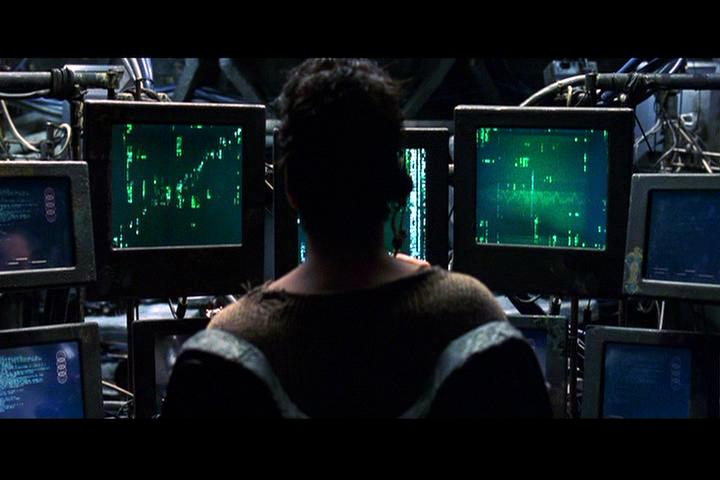
\includegraphics[width=0.5\linewidth]{fig/e7e946101bf652fcc2ce7923.jpg}
\end{figure}

\begin{myquote}
Roland: The machines have taken Junction 21. The way I see it, if we drop down from broadcast here, at Interstate 153, we might surprise them. We go first, hammer as deep as we can, them blow our EMP. Hopefully, we can punch a hole big enough for you to get through.

Niobe: *sighs*

Roland: It ain't pretty, but the way I see it, it's the only way back.

Niobe: No it's not. There's another way. A support line. It drops down right here. A thousand meters short of 21. If we're lucky, we may be able to slip down without them ever knowing.

Roland: That's a mechanical line. It's impossible. No one can pilot mechanical.

Niobe: I can.

Roland: Bullshit.

Niobe: I've done it.

Morpheus: That was a long time ago, Niobe.

Niobe: I said I can do it.

Roland: So what? If you can, you'll be the only one that can. There's no way we can follow you.

Neo: Hi. I know time is always against us, and I'm sorry I took so long. But I wanted to be sure.

Trinity: Sure of what?

Neo: I know what I have to do.

Morpheus: What?

Neo: There's no easy way to say this, so I'll just say it. I have to take one of the ships.

Roland: What?

Morpheus: To go where?

Neo: To the machine city.

Roland: *laughs*

Neo: I know it's difficult to understand ...

Roland: No, it's not --- you're out of your god damn mind.
\end{myquote}

God damn一词又出现了,说明Neo要上机器城完全是预料之中的。谁的预料之中呢?当然是先知。

\begin{myquote}
Neo: I still have to go.

Roland: You'll never make it. Hundred years no ship has gone within a hundred kilometers of it. You'll never make it.

Neo: I have to try.

Morpheus: Is this what the Oracle told you?
\end{myquote}

老莫的反应也很有趣,他一向是信仰先知的,即便在影片的开始他质问过先知。但是到了关键时刻,他还是要问一下是不是先知的计划。

\begin{myquote}
Neo: No.

Roland: This is asinine! If you want to kill yourself, go do it, but do it without wasting one of our ships.

Neo: You have to believe me. I have to go.

Roland: Bullshit! While I'm captain of this ship, I say where it has to go. Believe me, this ship will go to hell long before I let you take it anywhere.
\end{myquote}

“这艘船下地狱”很有趣。neverwin和郭大路都把Zion保卫战称作地狱之战,那画面就是炼狱图,而这艘船就是下地狱的那艘。

\begin{myquote}
Niobe: He can take mine.

Roland: You can't do that.

Niobe: Don't even think of trying to tell me what I can or cannot do with my ship after that little speech.

Roland: But for Christ's sake, Niobe ...
\end{myquote}

为了“基督”,这句话也是很有趣的。Neo就是这个救世主的角色,为了Neo, 那不就是把飞船给他?

\begin{myquote}
Niobe: I'll pilot this ship. He can take mine. If we leave inside an hour, we should reach Zion as the machines do. That's as good a plan as any.

Roland: It's a waste. A god damn waste.

Niobe: Two ships, two directions. Sounds like providence, doesn't it, Morpheus?
\end{myquote}

第二部里,Trinity告诉Neo说老莫和Niobe分手是因为老莫去见了先知,这个就是先知告诉老莫的,老莫一定是以为他们两人不同路。

\begin{myquote}
Morpheus: You've never believed in the One.

Niobe: I still don't.

Morpheus: Then why are you doing this?

Niobe: I believe in him.

Neo: Thank you.
\end{myquote}

这里要提一下Niobe名字的另一个不太为人所知的意思。很多人认为Niobe只是个神话人物,其实导演要暗示是Ebion(换一下字母顺序)。这类人不相信耶稣是上帝的儿子,但是相信耶稣确实是个特殊的人。这里Niobe说自己不相信救世主的预言,但是相信Neo的能力。

\myparsep

\begin{myquote}
Trinity: I'm ready.

Neo: Trinity ... There's something I have to say. Something you need to understand. I know I'm supposed to go. But beyond that --- I don't know ...

Trinity: I know. You don't think you're coming back. I knew it the moment you said you had to leave. I could see it in your face, just like you knew the moment you looked at me that I was coming with you.

Neo: I'm scared, Trin.

Trinity: So am I. Took me ten minutes to buckle up one boot. But I'll tell you something. Six hours ago I told the Merovingian that I was ready to give anything and everything for you. Do you know what's changed in the past 6 hours?

Neo: No.

Trinity: Nothing.
\end{myquote}

两人准备慷慨赴死,没有什么需要详细讲的。不过就是这里让很多人认为Trinity和Merovingian谈判那一段被删了些内容。其实很好理解,Trinity的意思就是“我对他说我愿意为你死,现在我还是一样”。而且Trinity和Merovingian谈判后的剪辑其实很不错,很多优秀的电影都用过切除重要片段的手法来为观众提神,不过这样的手法最早是美国漫画常用的手法。

讲讲欧美漫画充实版面吧。美国的漫画人其实和我们脑子里漫画人的概念很不同,他们往往都是很有阅历、很博学的,不是那种只会画两笔的小青年。特别是在80年代欧美漫画new wave之后的漫画人,基本上都有极丰富的科学知识,就连早期的《超人》也被他们用科学给解释了,NGC专门为《超人》中的科学制作过纪录片。而且他们还都是符号学的专家,不是鲍德里亚那种,而是具体使用的专家。他们放在漫画中的隐喻是很深的,不像是日本漫画总给你拿出来讲。另外还有很多人在专门知识领域里很有研究,最主要的几个领域是政治、科学、医学,像是导演(以前是写漫画的)这样的哲学类也有一些。我知道的少数几个哲学类漫画人现在都在导演门下,比如说Kaare Andrews,他为黑客帝国的漫画系列写了一个关于Kid的故事,名叫I Kant。光这个名字就很有意思,本意是“我做不到”(I can't),改了一下拼写就成了康德(Immanuel Kant)名字的缩写。要知道我在这里一直提的叔本华就受了康德很大的影响,据说他的书桌上就放着康德的画像。Kaare往故事里融合康德哲学很能说明他的哲学底子。而另一位Dave Gibbons的《Butterfly》还引用了老子的《道德经》,居然是直接引用中文的,真不知道有多少欧美漫迷看得明白,估计他们都根据那意境往佛教上理解了。

\begin{myquote}
Roland (v. o.): Are you finished loading that amunition?

Mauser: Just about, sir!

Roland: Let's move it, we are out of time.

Niobe: You're not leaving them anything?

Roland: Said he didn't need it.
\end{myquote}

看来Neo去机器城这个决定是做得很艰难的。一来他知道自己非去不可,二来他知道常规武器没有用。这时候的Neo就和面对Smith的先知一样,只能hope。

\begin{myquote}
Link: *hugs Trinity* I ain't saying goodbye. I'm saying good luck.

Trinity: Thank you.

Morpheus: I can only hope you know what you're doing.

Neo: Me, too. It was an honour, sir.

Morpheus: No, the honour's still mine.
\end{myquote}

在哲学家那条音轨里,Ken和West说这时候的Morpheus终于是个真真正正有血有肉的正常人了。第一部里的Morpheus是神,他告诉我们现实;第二部里的Morpheus是父,他带给我们希望;第三部里的Morpheus是人,为了自己的选择而战斗。老莫在这里的说的honour才是真正被我们感知的那个honour。第一部里戴着反光的墨镜,露出捉摸不透的笑容,那时候哪里有观众感受这个词啊,都在猜老莫是个什么人呢。这里的honour才是一个战士嘴里的honour。

\begin{myquote}
Mauser (v. o.): We're ready, sir.

Roland: 'Bout damn time. *to Niobe* We're already late, captain, so let's hit it and hit it hard.

Niobe: Bye, baby. Take good care of them.
\end{myquote}

女武神要出发了,Logos也要去机器城了。先知的这个预言拆散了老莫和Niobe,但是好在有些事是不会变的。

\begin{figure}[htb]
\centering
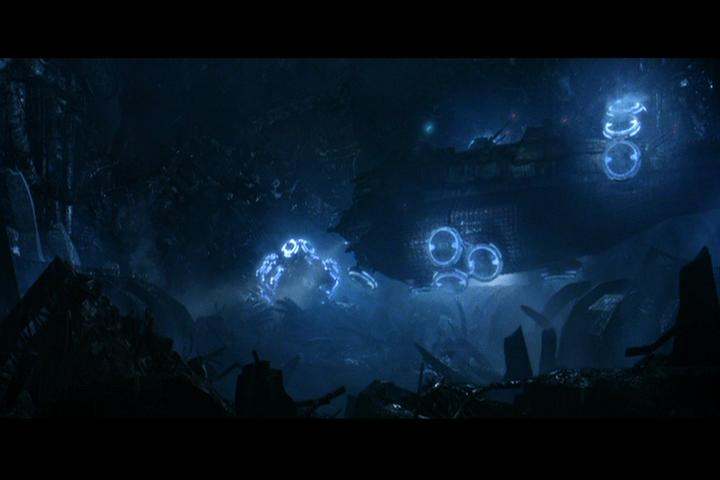
\includegraphics[width=0.5\linewidth]{fig/0c47bd3135fd92a85fdf0e64.jpg}
\end{figure}

\begin{myquote}
Trinity: Ready?

*Neo nods. Trinity punches a button and the lights go out*

Trinity: Engine's still firing. Must be a fuse. I'll check it out.

Bane: I should've known he'd sent his bitch first.

Trinity: Bane?!

Bane: No one ever got away from me as many times as you did. Every single time I thought it was the last. Every time I was sure we had you, but somehow you'd slip through our fingers. I really can't express just how aggravating that can be.

Trinity: What are you talking about?

Bane: I think I might enjoy killing you as much as killing him.

Trinity: Neo! It's Bane, he's psychotic!

Bane: You're gonna pay for that.
\end{myquote}

这个Bane的本意是毒药、祸害,应该不用解释意思了吧。很快我们就要看到黑客帝国三部曲中最真实的打斗了。

\begin{myquote}
Ghost: Twenty-seven kilometers to go.

AK (v. o.): Captain, we've got an emergency down here.

Roland: What is it, AK?

AK: It's Maggie, sir. She's dead. Murdered. I think it was Bane.

Roland: God damn it.
\end{myquote}

又是god damn it, 又是注定的。但是话说回来,什么不是注定的呢?

\begin{myquote}
Roland: I knew it. I knew he was out of his god damn mind. He fired that EMP. God damn it, I should have beaten it out of him.
\end{myquote}

这里的out of mind也很有意思。Smith的mind本来就是在Matrix中,现在溢出到人体里,字面上理解也是out of mind。

\begin{myquote}
Colt: We've searched the whole ship, captain. He ain't here.

Roland: I know where he is.

Morpheus: The Logos.

Link: We gotta go back!

Roland: Too late.

Link: You don't know that. What if they need our help?

Roland: It's too dangerous.

Link: Why?

Morpheus: Because if he's killed them, he'll control another EMP.

Roland: At this point, they're on their own ... just like us.

Bane: Mr.~Anderson. I see you're as predictable in this world as you are in the other.
\end{myquote}

在《黑客帝国》里,说一个人容易预料可以算是最大的侮辱。但事实上,Neo确实很容易被预料,因为Smith理解他和Neo的使命。第一部里Smith还是个特工的时候就很好地预料到了Neo的行踪,在Jones和Brown在下面追赶Neo的时候,Smith就已经在303房间等候他了。

\begin{myquote}
Neo: What?

Trinity: He's out of his mind.
\end{myquote}

这句out of mind又出现了。一语双关的例子在第一部Neo挨老板骂的时候就已经发挥到了极致。这里要纠正一点(也不算是纠正啦,提一下),我在补充neptuneneo的第一部解读的时候说他老板Rheinheart的名字是来自一位康德派的哲学家,曾经出现在黑格尔的《大逻辑》中;而这个名字现在有了新的解释,这个名字可能来自瓦格纳的歌剧Das Rheingold。因为第三部中有四首配乐的名字对应瓦格纳的《Der Ring des Nibelungen》(尼伯龙根的指环),Das Rheingold正是其中之一。此外,这里的配乐就叫做Das Banegold。

\begin{myquote}
Bane: It might appear that way to you, but Mr.~Anderson and I know that appearances can be deceiving. Confused, Mr.~Anderson? It'll all become clear in a moment. Now, thank you for bringing me the gun. You can set it down right there.
\end{myquote}

这段话第一句是很重要的,黑客帝国官方网站上有一整篇文章就是讲的“对你来说,对我来说”的问题,那位教授用这一点分析了Matrix内外的真实性。而在这里,意思就是个体和对象的转换造成概念指向的差别。

而这里的“appearances can be deceiving”已经成了我一位文学老师的课程之一,关于这一点就不用多说了。笛卡尔的恶魔论、莱布尼兹的单子论、鲍德里亚的后现代、黑格尔的感性确定性、叔本华的表象世界,还有印度教佛教的maya(摩耶)、samsara(轮回)、圣经传道书的空虚为本等等都指出“表象的欺骗性”,也有说表象的作用是“藏起其实不存在的事实”。

\begin{myquote}
Trinity: Don't do it. Shoot. Shoot now.

Bane: Yes, shoot, fry us, burn us alive!

Trinity: Shoot, Neo. If you don't, he'll kill us both.

Bane: Look at him. He knows he should do it but he won't. He can't.

Trinity: Do it.

*Neo puts the gun down*

Bane: Back away from the gun and turn around.

Neo: Let her go.

Bane: Somehow familiar, isn't it? We've been here before, you and I. Remember? I do. I think of nothing else.
\end{myquote}

这里Smith说的就是在第一部里杀死Neo的情形。前面已经提到过了,Smith再生之后一直想的就是复仇。

\begin{myquote}
Neo: Who are you?

Bane: Still don't recognize me? I admit, it is difficult to think, encased in this rotting piece of meat. The stink of it filling every breath, a suffocating cloud you can't escape. *spits blood* Disgusting! Look at how pathetically fragile it is. Nothing this weak is meant to survive.
\end{myquote}

又和第一部呼应了,Smith在审问老莫的时候就说过他讨厌人类的味道,又开始谈论人类不该存在的理论了。

然而,我觉得现在是时候解答neverwin在第二部解释中留下的一个思考题了:法国人看到Neo流血后说的“看,他只是个人”是什么意思?

这个问题应该和Smith在自己手上划伤痕联系起来解释。圣经中,彼拉多把耶稣交给犹太人时说了ecce homo,也就是“看这个人”。这句话有两种意思,一是“看啊,这就是那个人”,这个用法被尼采采用,写下了《Ecce Homo》一书;另一种用法是“看啊,他还是个人”,在耶稣受刑的时候,人们看到创造奇迹的耶稣也会受难,所以说他还是个人。

法国人看到Neo流血而说的“看啊,他还只是个人”就是ecce homo的第二种用法,当然也暗示他是救世主。而Smith也一样,他刚刚进入Bane的身体要适应“自己是人”,感受痛苦就是他感觉自己是人的方法。当然了,他还是向往变成神更多一点。

而ecce homo的第一种用法也在电影中使用了。配乐大师Don Davis曾经说到过Neo和Smith大战时的配乐,尼采的《Ecce Homo》是一个候选,后来因为效果问题才最终选择了《奥义书》。(《神曲》原本也是个选择)

\begin{myquote}
Neo: What do you want?

Bane: I want what you want.

*Neo looks up with recognition in his eyes*

Bane: Yes ... That's it, Mr.~Anderson. Look past the flesh, look through the soft gelatin of these dull cow eyes and see your enemy.

Neo: No.

Bane: Oh, yes, Mr.~Anderson.

Neo: It can't be.

Bane: There's nowhere I can't go. There's nowhere I won't find you.

Neo: It's impossible.

Bane: Not impossible. Inevitable. Goodbye, Mr.~Anderson.
\end{myquote}

“不可能”和“必然”的问题又出现了,“不可能”的本质就是按过去经验对未来预测的准确度极低,而“必然”的本质就是因果律所指出的。再给一个拉丁谚语吧:Certum est, quia impossibile(这是必然的,因为这不可能)。这在第一部也提到过了,Trinity对Neo说从没有人能这样从特工手中救出人,Neo说:“所以这是可行的。”

\begin{myquote}
Trinity: This is it, it's gotta be. *She pushes a circuit breaker, the lights go out*

*Bane/Neo fight*

Neo: *screams*

Trinity: Oh, no.

Bane: I wish you could see yourself, Mr.~Anderson. The blind messiah. You're a symbol for all of your kind, Mr.~Anderson. Helpless, pathetic. Just waiting to be put out of your misery.
\end{myquote}

这里有个明显的隐喻——弥赛亚,和大喊“Jesus Christ”的用法没多大差别,唯一的小区别就是犹太人恨耶稣,但是企盼弥赛亚的到来。Smith这么一说,就是把不完整的救世主给说完整了。Neo不再只是人类的救世主,而是Matrix和人类共同的救世主。

\begin{myquote}
Neo: I can see you.

Bane: It's not over, Mr.~Anderson. It's not over.

Neo: Trinity!

Trinity: Neo. Oh, no. Your eyes.

Neo: I'll be okay. It's all right, Trin. But I think you're gonna have to drive.
\end{myquote}

\begin{figure}[htb]
\centering
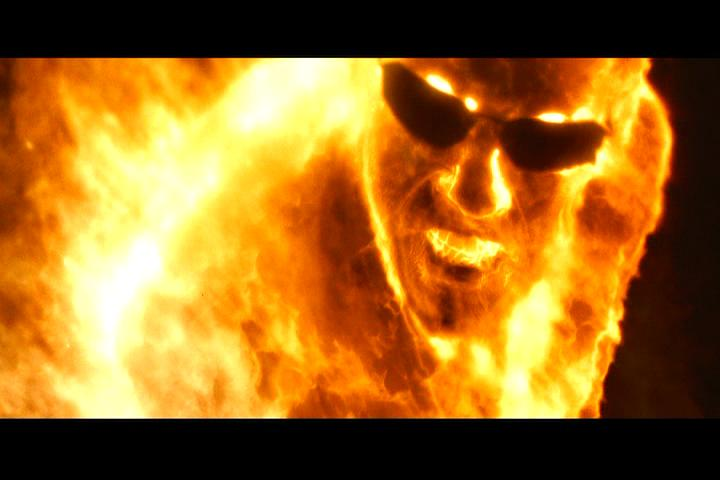
\includegraphics[width=0.5\linewidth]{fig/f64563d00ca0378fa1ec9c63.jpg}
\end{figure}

这个金色的Smith以及后面的金色机器可以算是黑客帝国中最难理解的。这个难不是因为理论的深,而是因为这里不科学。事实上,这里是黑客帝国三部曲最纯粹的哲学表现,不带有丝毫的杂物(呵呵呵,不是说我自己)。鲍德里亚曾经批评《黑客帝国》对他的理论有误解,拟仿物和拟像的关系并不是显而易见的,并不是可以概念化的。鲍德里亚说这件事的时候,只有第一部上映了,所以说鲍德里亚很自然地认为Zion和Matrix是拟仿物和拟像的关系,电影中二者却被清晰地赋予了概念,这就是他觉得“误解”的地方。事实上,真正的拟仿物根本没有在第一部电影中出现。

而分析哲学家,和鲍德里亚代表的后现代主义者一直处于对立位置的那些,按他们自己的分析法来指出《黑客帝国》很好地代表了哲学的后现代主义(他们说其中传统哲学比后现代更为优秀),并批评鲍德里亚用词晦涩难懂,似是而非地回答问题等等缺点,说他们说话的方式比他们说的话更重要。

我个人觉得鲍德里亚的难懂是很正常的,既然拟仿物和拟像的关系非常不明确,或者如其他理论说的拟仿物根本不存在,鲍德里亚若是使用十分清晰的字眼就更容易出现读者的误读,倒是导演这种视觉做法很容易解释哲学的后现代。

这个金色的Smith才是三部曲中唯一的拟仿物。既然拟仿物是超越我们感官的,那么我们就看不见这些东西。而导演安排Neo在眼瞎之后看到真正的拟仿物,很明显是告诉我们这个金色的Smith是个表现形,是超越我们视力的。叔本华说过我们视野中的任何东西都不能证明我们是在用眼睛看,这就是允许这个逻辑矛盾存在的依据。

我们黑迷在谈到金色光芒的时候,习惯管这叫精神、灵魂,我认为这更像是莱布尼兹所说的“单子”,或者是黑格尔感性确定性中那个不存在的“完美概念”,也可以是柏拉图洞穴寓言中无限真实的“Good”,也可以是印度教中的“涅槃”,也可以是《传道书》中说的空虚,也可以是真实的缺失的表现。但是,我们看到的画面又绝对和我上面提到的这些理论不一致,因为这是不能被概念化的。任何一种对金色光芒的解释都是错误的,我们唯一能做的就是给它取个名字,不能叫“灵魂”,因为灵魂和莱布尼兹的“单子”太接近了;不能叫“意志”,意志极抽象,但是富于概念性;应该叫“精神”,因为精神的概念是很模糊的,机器的精神就更为模糊了。如果叫做“灵魂”的话,就肤浅了,因为那会被理解为机器的信息层面;如果叫“意志”,那就偏差了,因为那会被理解为机器的自主目的。所以“精神”是迄今为止最好的叫法。当然,最好的表现法仍然是电影中直接的表现法,把机器的“精神”嵌入逻辑的矛盾(瞎眼的视野)中,致使我们无法定义它,又让观众有了个直观的感受。

除了电影中的做法,任何其他对拟仿物的描述都是偏差的、肤浅的。“机器的灵魂”是肤浅的,“机器的意志”是偏差的,“机器的思维”是狭隘的。《黑客帝国3》对模仿和拟像的描述是不可超越的,就连鲍德里亚本人也不能超越《黑客帝国3》,因为他仍然用文字,他仍然使用定义归纳。《黑客帝国3》不仅是后现代拟像描述的典范,还是后现代拟像描述的极至!难怪那个分析哲学家Richard Hanley说如果他也拍电影解释的话,根本不会把鲍德里亚放在眼里。

但讽刺的是,这种极至的哲学看上去和哲学没有多大关系,要接近理解(完全理解是不允许的)它需要绕一个哲学的大弯才行。

\myparsep

\begin{myquote}
Lock's Lieutenant: Seismic's projecting twenty-two minutes to breach.

Lock: They can't know we don't have an EMP, they'll have to attack in waves. Concentrate our offense on the diggers. Order the APUs into position.

Lock's Lieutenant: Yes, sir.
\end{myquote}

最高指挥官Jason Lock和老莫是情敌,估计是他和Niobe一样不相信救世主才走到一起的。所以说当Niobe说他相信Neo的时候,也是Niobe和Lock划清界限的时候。

根据Matrix Dictionary的说法,他是唯一一个有全名的Zion人员。这个家伙是个hardass,很多船员都管他叫deadbolt(主要是Logos的接线员Sparks这么叫他)。这个外号和他的名字其实很相配,lock是锁的意思,bolt是门闩的意思。作为Zion的指挥官,他的任务就是锁住Zion的大门。

另外,Lock也是暗示一个英国的哲学家John Locke。他虽然不是自然哲学家、形而上学家,但也研究认识论,和伯克利等人被归类为经验论者,这点对黑迷来说应该不会陌生,我翻译的《哲学家探索黑客帝国》一书中就有关于伯克利哲学和《黑客帝国》的文章。总的来说Locke是个很务实的人,指挥官Lock也一样。

而他的名字Jason则是一个希腊神话中的英雄的名字,伊阿宋。呵呵,不知道怎么出现的这个音译,可能古希腊语的发音和西班牙语很接近吧(J都是发Y的音)。

\begin{figure}[htb]
\centering
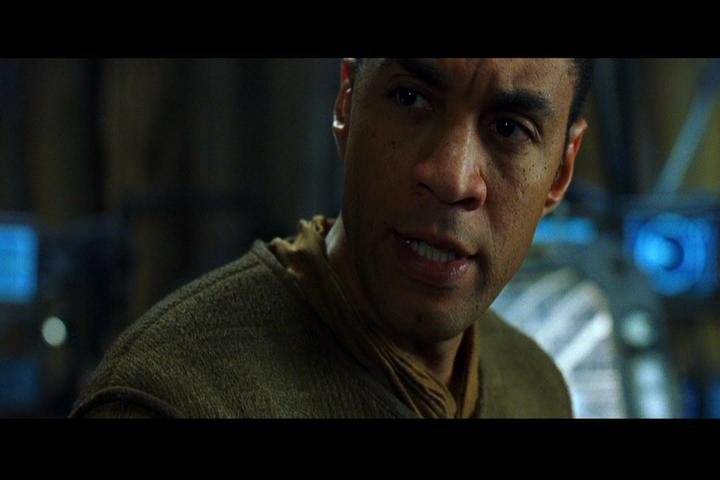
\includegraphics[width=0.5\linewidth]{fig/5fe264383ee43a2397ddd8f2.jpg}
\end{figure}

\begin{myquote}
Mifune: All right, this is it. Now, you all know me, so I'll just say this as simple as I can. If it's our time to die, it's our time. All I ask is: if we have to give these bastards our lives, we give 'em hell before we do!

APU fighters: *cheer*
\end{myquote}

这个APU的意思是Armored Personnel Units,据说这个设计在现实中也有很高的可行性。而Mifune这段战前宣言也够简短的,但是很有气势。导演俩拍电影废话没有一句,该说的就说,不该说的就不说。这样的结果是很有趣的,比如那些哲学探讨,看电影不带脑子的人看着就惨了,一大段一大段的东西根本消化不了,而正好研究这种理论的哲学家们就对这些谈话感到无聊了。(还好《黑客帝国》不是我拍的,我得把每样东西讲得格外清楚才罢手,估计没几个人受得了)

\begin{figure}[htb]
\centering
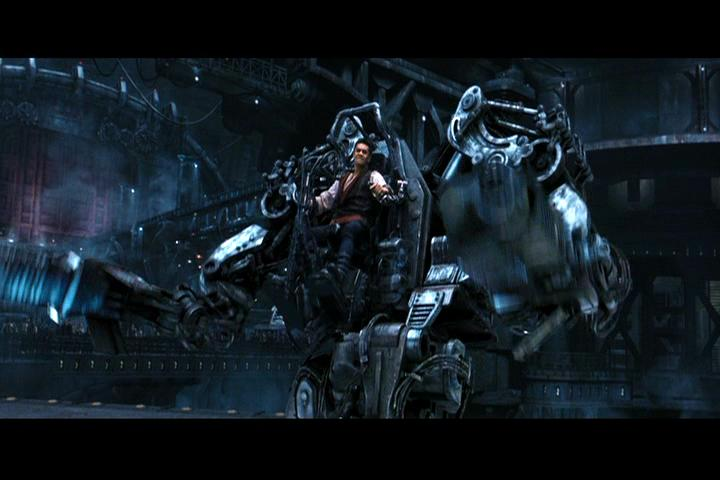
\includegraphics[width=0.5\linewidth]{fig/385658828a847ba20cf4d2f2.jpg}
\end{figure}

\begin{myquote}
Zee: You scared, Charra?

Charra: Shit, yeah. I'll make you a deal, though. You keep loadin', I keep shootin'.

Zee: Deal.
\end{myquote}

接线员Link的老婆Zee加入了Lock征求的志愿者,和她一组的Charra名字是西班牙语女牛仔的意思。

这一段从Lock开始到Zee这里的一段戏描写的就是Zion的各个阶层对Zion大战的准备。这个被neverwin和郭大路称为末日之战的大战中,也是有很多隐喻的,不过哲学内容少了,所以Ken和West在制作音轨的时候没有对这里进行多少评论。我在这里主要也就是挖些隐喻出来。

\begin{figure}[htb]
\centering
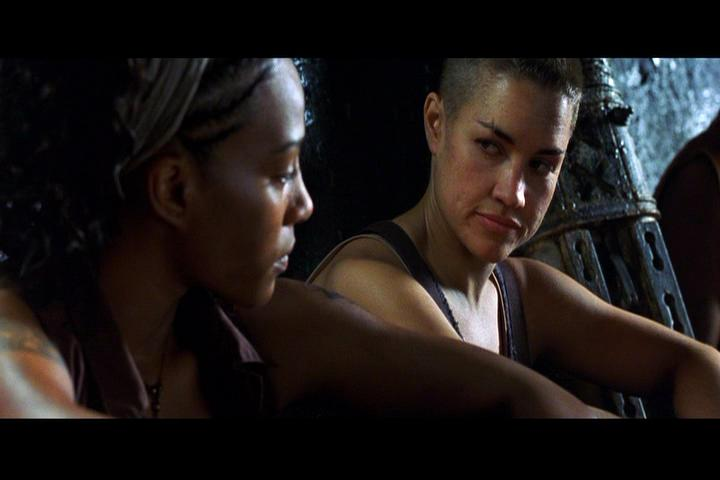
\includegraphics[width=0.5\linewidth]{fig/27d5d1a236c79aadcbefd0f2.jpg}
\end{figure}

\begin{myquote}
AK: Holy Christ. Would you look at that?

Roland: Quiet. [How far down?]

Ghost: 1.4 kilometers.

Morpheus: Still generating too hot field.

Niobe: Ghost, kill all auxiliary systems. Give me full manual, drop down to four pads.

AK: It'll bottom out!

Niobe: Easy, baby.

Ghost: 700 meters.

Niobe: If we can just get close enough.

Ghost: 600 meters.

AK: There.

Niobe: Shit!

Ghost: Jig's up, here they come.

Niobe: Give me full power, full systems!

Roland: Man the gun turrets, every goddamn one of 'em!

Niobe: Ghost, you're the best gunner we have, go with them. Morpheus, take his place!

Link: I'm comin', baby.

Morpheus: Here they come.

Roland (v. o.): Slow down, this ain't the Logos!

Niobe: Hold on to your lunch, Roland, here we go.

Roland: Holy Christ! Didn't know this ship could do that.
\end{myquote}

现在他们要做的就是抢时间。Morpheus在第一部就说“时间总是和我们作对”。我在火车站的场景中就说过了,导演对摩耶三限制“空间、时间、因果”的刻画是很注重的。我们在看电影的时候可以注意到,自从Neo第一次进入Matrix,他们总是在和时间赛跑,无论是从先知那里出来躲避特工,在Cypher杀死Neo之前干掉Cypher,还是在老莫招供之前救出他,或是在乌贼杀死他们之前接起303房间的电话。Nebuchadnezzar在第二部里36小时的充电也是匆忙的(老莫下船时就叫Link尽快准备),Neo准时去见先知,又必须在12点整见Merovingian,在高速公路上救起就要被火焰吞没的老莫和Keymaker,Trinity要在他们进入大楼前破坏电力设备,Neo要在Trinity坠楼之前接起她,Nebuchadnezzar的船员还要快速撤离要被炸毁的飞船。到了第三部,完全就是建立在赛跑上的。

所以老莫说的“always”就是字面上的always!他们就是永远和时间赛跑的人。

赛跑中有些很有趣的细节,比如Link对这条手链的态度改变。根据Link在第二部中和Zee的对话,我们知道他并不相信救世主的说法,他来当接线员是因为他对Dozer发过誓,然而他在看到Neo的能力之后开始相信了。而在Neo和Smith的最终大战之前,他说了一句:“Neo, if you gonna do something, you better do it quick.”他完全把Neo的胜利当作时间问题了。

这和手链的信仰是一模一样的,从开始的“你知道我不信这套的”到第二部的“戴着也无妨”到这里的“宝贝,我回来了”。Link就从Niobe一样的无神论转变到了Morpheus的深度信仰。

\begin{figure}[htb]
\centering
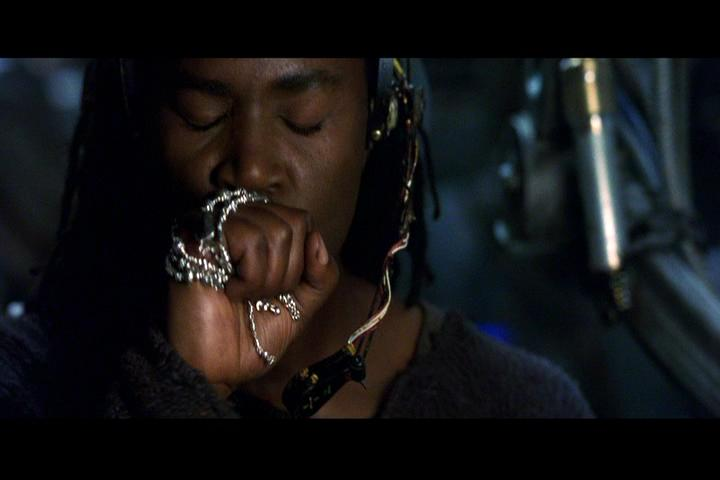
\includegraphics[width=0.5\linewidth]{fig/aea59e3d72117d00bba16754.jpg}
\end{figure}

图片可能不清楚,这里是一个大个头的乌贼先出来定位,然后一大群小型的乌贼就冲出来了。在幕后花絮里,工作人员说过他们设计了很多不同种类的乌贼,因为导演很注意“目的”,所以就需要很多有不同“目的”的乌贼来打这场仗。其实乌贼的15条触手都有不同的用处。(种类不同,触手数也可能不同,花絮碟里提到的是15个触手的那种)

“目的”可以说是《黑客帝国》最主要的主题,Neo和先知就“目的”的问题大谈过一场。我们常说的“意义”就是目的的一个变体。Sati是因为没有目的而面临删除,Merovingian一帮人因为目的过期而面临删除,Keymaker因为目的完成而被删除,第一部里的特工Jones和Brown因为目的完成失败而被删除。总之,机器的存在是有目的的。而人类呢?虽然尼采批判过consensus sapientium(智者的一致),而且就是对“人生没有意义”的批判,但是大多数哲学家都认为生命是没有目的的(不知道为什么罗素说叔本华是唯一的悲观哲学家)。

按照亚里士多德的原因论,任何事物都有质料因、形式因、动力因和目的因,而他最主要讲的就是目的因中的自然目的论(和意义有很大区别)。他说过:“如果看不见运动者有意图,就不承认有目的因存在,这是荒谬的。”(呵呵,看不到黑客帝国的哲学就说没有,这也是荒谬的)所以人类的存在是有目的的,但这是自然目的,因为人类的诞生并非意识的结果。而像尼采这样赋予人生以目的或是意义,则是人为的目的论,是技术目的,是行为目的。

尽管人类的存在没有意义(我说过我是叔本华派的,你当然可以不同意),但是Neo也有足够理由保护Zion。既然任何存在都没有意义,那么“不存在”也绝无意义可言,那么机器毁灭人类虽然有技术目的,有行为目的,但是并非自然的(即使是进化所需,也不用赶尽杀绝)。

这也就是我在解释Revolutions这个标题时说的关于程序和人类固有目的的革命。

\begin{figure}[htb]
\centering
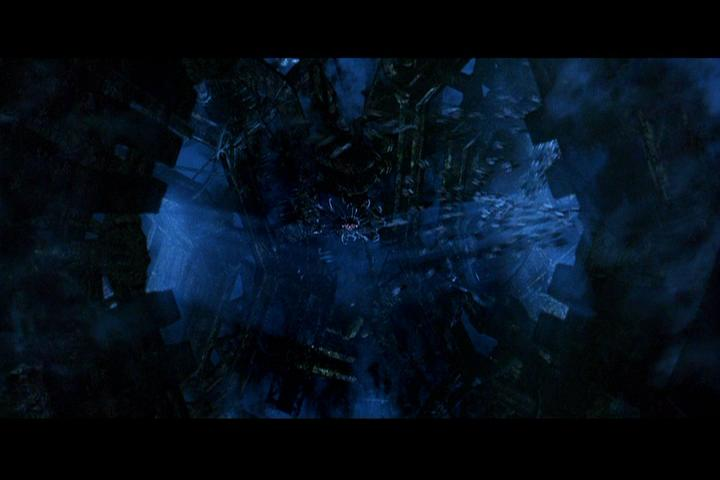
\includegraphics[width=0.5\linewidth]{fig/d272b81259316fcec2fd7854.jpg}
\end{figure}

\begin{myquote}
Operations Officer Mattis: Breached! The dock is breached!
\end{myquote}

首先,这个官员名字,Mattis, 指的是美国海军陆战队一位著名中将James Mattis,研究中东局势、伊拉克战争的人都应该听说过这个名字。

Zion被突破,一个巨大的digger掉下来,这个digger的造型就是倒置着的巴别塔。圣经的创世纪中记载人们想要造一座通天的巨塔,上帝怕人们齐心就可以做到任何事情,所以就使得人们说不同的语言,让人们之间不能交流,结果这座塔就没有建成。巴别塔的作用原本是通天,而在Matrix中,Zion才是真实的世界,是天堂,所以digger就像是倒置的巴别塔一样挖到Zion。此外,巴别塔的意象在1927年的《大都会》中也出现了。

巴别塔最初的原型被认为是Tower of Jupiter Belus,即巴比伦的米罗达之塔。而有趣的是,建造这座塔的人就是我们所熟知的Nebuchadnezzar,老莫飞船的名字嘛。

\begin{figure}[htb]
\centering
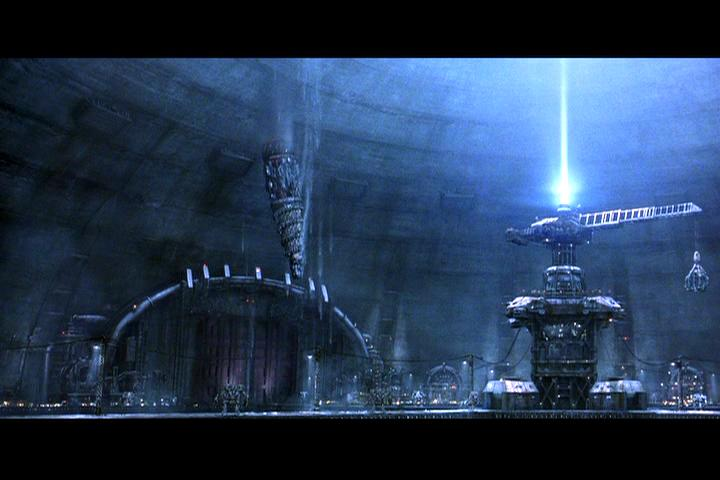
\includegraphics[width=0.5\linewidth]{fig/9f1903089ad2bcd162d986ee.jpg}
\end{figure}

\begin{myquote}
Mifune: Knuckle up!

*The sentinels start coming through the breach*

Mifune: For Zion!
\end{myquote}

Zion大战正式开始,Mifune带领他的APU战队进行反抗。现在的乌贼还卡在瓶颈里,几百台APU的枪口都对准着这一个地方。这是很能体验结构美的场面,相信喜欢这一段的朋友都是在欣赏结构美,爆炸的机器、露出的电路、碎开的零件。欣赏结构美者往往习惯于内省和思考,创造结构美者更是如此。欣赏结构美是不断从自己的经验中提出可能的发生进行和变现的对比,不断依靠思维的空间创造力体验结构的精确性和科学性。呵呵,从电影中,我们这样的cult不但可以学习到很多东西,还可以研究一下导演俩本身的特质。

\begin{figure}[htb]
\centering
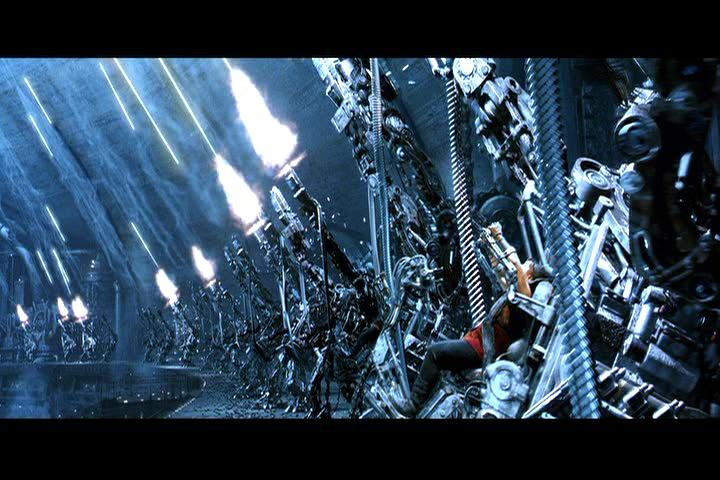
\includegraphics[width=0.5\linewidth]{fig/b5c64723f3d126529822edee.jpg}
\end{figure}

再一次出现“目的”的重要性展示,这些乌贼的目的就是牺牲自己,保护挖掘机。但是乌贼对目的的理解不像是Keymaker的那种理解。Keymaker那种中庸的思想,那种接受命运的态度很容易被理解,也很难被理解。容易是因为这种思维方式就是一种人类的思维方式,难在于没有多少人可以真正领会接受命运的人生观。而这些自杀式的乌贼根本就没有多少智慧,甚至不能说是智能。这些乌贼没有求生的能力和欲望,它们的所作所为是程序控制着的,这种自杀行为的根据是“1、躲避会使自己受到伤害的进攻;2、冲向会使挖掘机受到伤害的进攻,第1条此时作废”。不存在思维进程的乌贼只是有极大广度的行为回应覆盖率,换句话说,能够处理所遇到的绝大部分情况,但是并不存在自主的思维能力。

\begin{figure}[htb]
\centering
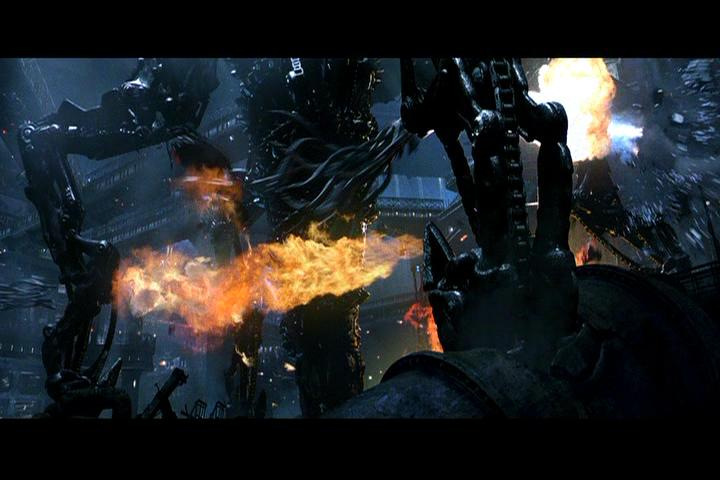
\includegraphics[width=0.5\linewidth]{fig/ee8e55e709f6992eb93820ee.jpg}
\end{figure}

数字3再次出现。导演俩对于3的偏好来自于但丁的《神曲》,这一点并不令人吃惊。《神曲》作为配乐师Don Davis的候选配乐,火车站对于Limbo的暗示都很清楚地体现了导演俩对《神曲》的偏爱,digger的外形和《神曲》中所描述的地狱外貌也很相似。《神曲》分为《地狱》《炼狱》《天堂》三部分,每部分33首歌,加上一首总的序曲,总共是100首。而《神曲》中描述的地狱、炼狱、天堂都有9层,但丁在写作的时候使用的是三韵句。

当然,你也可以说这为的是一种结构美。的确,三个特工一组,三个黑客一组,三条船一组,三个APU一组,这样的组合确实可以用结构美来解释。但是有时候对于3的运用和结构是没有关系的,比如说Trinity的房间号为303,Neo和Smith在地铁站里的战斗都是在3号站台进行的,Hammer回到Zion用的是3号门。这些使用都是对数字3的直接使用,而非3的结构。

\begin{figure}[htb]
\centering
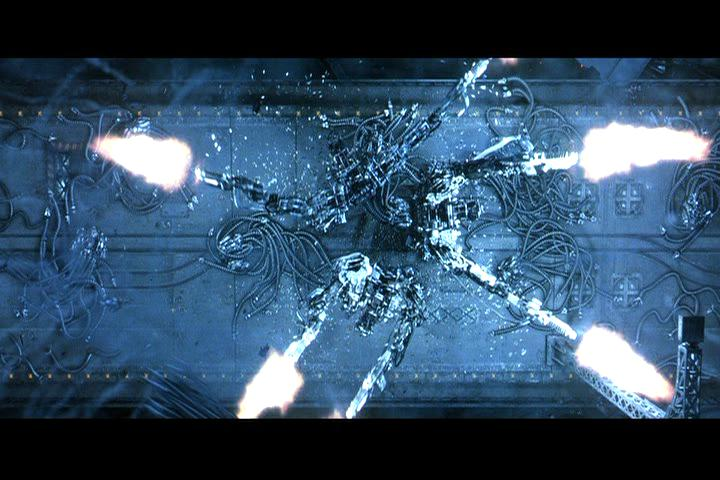
\includegraphics[width=0.5\linewidth]{fig/0874fcfae17645deb48f31ee.jpg}
\end{figure}

乌贼发挥数量的优势,从一个小小的洞口中一下涌了进来。乌贼总共有六个分支,6这个数字在《黑客帝国》中也很重要,这是第六个Matrix版本,也是第六个Zion,那个Merovingian是法国六代封建王朝第一代国王的名字,101又是第六个二进制数字,原剧本里Neo是老莫的第六个候选人,开锁人门边有6条横杠。关于数字6的解释一般是上帝创造世界用了六天。此外,耶稣在死后有六次显现,他还六次强调“寻找者就可以找见”(这在《多马福音》也有两次提及)。6还有一个特性就是1、2、3三个数的和与积都是6,所以被称为“完美数”。

\begin{figure}[htb]
\centering
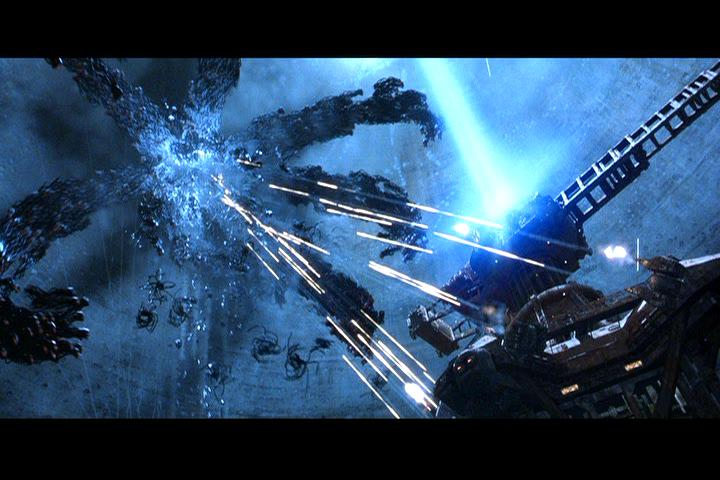
\includegraphics[width=0.5\linewidth]{fig/2fc3cc11f0d8ff10b9127bd2.jpg}
\end{figure}

\begin{myquote}
Radio Bunker Man: Reload Nine!

*Sentinel is shot down by the gunners in the ammo compartment*

Radio Bunker Man: Go, go, move, move!

Mifune: Watch the left! Don't let 'em through! *One of the APUs falls from the bridge* Zuka!

*A huge sentinel swarm moves towards the tower*

Tower Soldier: Oh my God.

*Sentinels swarm the tower, knocking down the tower gun*
\end{myquote}

通天的光柱被大群的乌贼毁掉。这个光柱和整个Zion船坞的穹顶设计参考的是罗马的万神殿。万神殿中的光柱不是人造的,是穹顶中有一个大洞,阳光从中照射下来,这个洞象征着上帝和人类世界的联系。穹顶上还有很多不同的神像,在《黑客帝国》中自然是没有什么神了,什么神像、什么神和人的联系通通被拿走,留下的只是象征人类自己生存奋斗的光柱。罗马万神庙的正式名称为Santa Maria ad Martyres,意思就是圣母与诸殉道者的教堂。这个地方还是伟人的公墓,比如文艺复兴三杰之一的拉斐尔就葬在这里。而在电影里,这里也确实即将成为伟人的公墓。

关于万神庙,有一点是很奇怪的,万神庙早在耶稣诞生前就已经建成,但这座神庙被送给教皇博义四世之后,他却没有对其中任何神像动手,只是改了神庙的名字而已。可能是因为当时基督教还不是很有规模,比如当时很多最具备深刻知识和理解的高等教士都信仰诺斯替(关于黑客帝国和诺斯替的关系会在后面详细解释)。但是,把众神当作圣母玛丽的殉道者,这还是很奇怪的。(比导演揉合各种宗教思想还奇怪吗?)

\begin{figure}[htb]
\centering
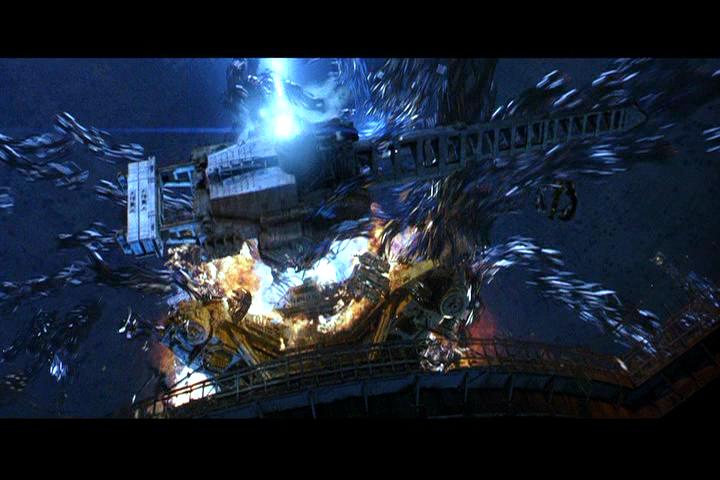
\includegraphics[width=0.5\linewidth]{fig/14a938db21aeea66d0164ed2.jpg}
\end{figure}

之前,Charra和Zee已经炸断了这个digger的一条腿,但是凭借着三条腿的稳定性,还是站着不倒。现在她们转到了挖掘机的另一面开火,这个大家伙就倒下了。这里导演为了缓解一下观众紧张了好几分钟的情绪,还给Lock他们安排了一个小包袱。

\begin{myquote}
Military Personnel: Yeah!

Operations Officer Mattis: 72 at the breach point.

Lock: God damn it!
\end{myquote}

\begin{figure}[htb]
\centering
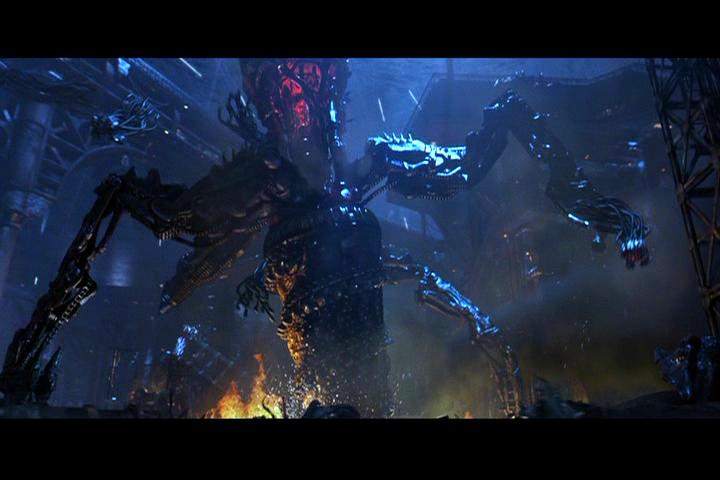
\includegraphics[width=0.5\linewidth]{fig/295cb035588b3a8ba61e12b0.jpg}
\end{figure}

\begin{myquote}
Niobe: Shit, she's got a fat ass.

*Sentinels swarm over the hoverpads of the Hammer*

Niobe: Keep 'em off me!

Roland: [God damn], there's a shitload of 'em.

Mauser: Captain! Do you see that?

Roland: They're [going for] the radio, stop 'em!

*Sentinels take out radio*

Roland: Damn it. [One print version]
\end{myquote}

Niobe第一句是说Hammer号太大了,以至于飞行十分困难。她原来开的Logos是所有飞船中最小的(原设计中,还有艘Bug Ship更小)。

这些乌贼很清楚如何对付飞船,它们要破坏飞船的通讯设备,这样Hammer就无法和Zion的战斗人员获得联系。机器的第二个目标就是破坏飞船的飞行pad,下图中可以看出发动机被破坏的程度。第三个目标就是破坏枪械设备,后面我们会看到Roland控制的机枪和一个radio被乌贼扯下来了。

\begin{figure}[htb]
\centering
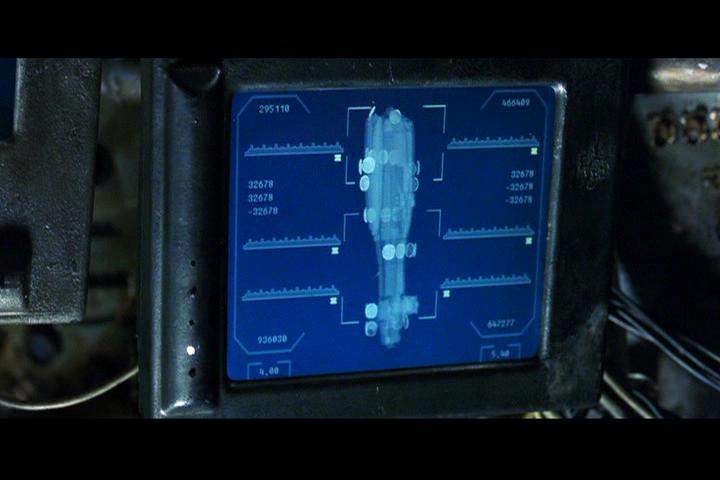
\includegraphics[width=0.5\linewidth]{fig/d456960a423f9d1f95ca6bb0.jpg}
\end{figure}

\begin{myquote}
Charra: Yeah.

*Charra positions herself on the edge*

Charra: Grab my belt.

*Zee grabs her belt and Charra hangs over the precipice*

Charra: Just give me one clean shot.

*Charra shoots, but fails to find her intended mark*

Charra: Shit.

Zee: Charra!
\end{myquote}

她们没能破坏第二台挖掘机,而Charra则被乌贼杀死了。下图是Charra和Zee准备从上面袭击挖掘机的画面。这正好是个诺斯替的符号,类似Sun Circle,外面的乌贼围一个大圈,挖掘机的四条腿形成十字形,中间是挖掘机主体的圆形。其实现在中间的这个小圈已经没有了,古代画法中还保留着这个小圆心。如果说十字是伸出圆外的,那么这就是一个凯尔特十字。当然,外面的大圆和里面的小圆可能不算在符号之内,这个符号就可能是指Saltire,也就是圣安德鲁十字。

\begin{figure}[htb]
\centering
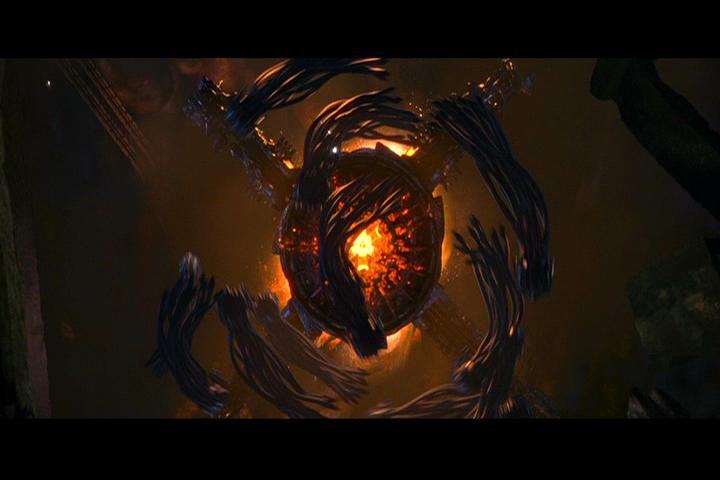
\includegraphics[width=0.5\linewidth]{fig/32e4c817074fdf09c93d6db0.jpg}
\end{figure}

\begin{myquote}
First Operator at Command: Commander Lock, I've got incoming!

Lock: I got a dock load of incoming!

First Operator at Command: Sir, yes, sir, but this is different, sir.

Lock: What?

First Operator at Command: I think it's one of ours.

Lock's Lieutenant: The holographics are trying to confirm, sir.

Lock: Contact them, I want access codes.

Lock's Lieutenant: We're trying, sir, there's no response.

Lock: It's a trick. That's not one of ours, it can't be. That's a mechanical line. No one can pilot mechanical.
\end{myquote}

剪辑师Zack在这里的剪辑很有趣,当Lock刚说完“没有人能在机器通道行驶”,画面就切到了Niobe。在哲学家音轨里,Ken和West一起笑着接Lock的话茬说:“Except the warrior princess.”

\begin{myquote}
Niobe: Fore and aft --- 30 degrees, 80 percent!

Morpheus: 30 degrees, 80 percent.

Niobe: Fore starboard, 60 degrees, 20 percent.

Morpheus: 60 degrees.

Niobe: Come on, keep up!

Morpheus: I'm trying!
\end{myquote}

很显然,老莫的驾驶水平还比不上棕发女武神,速度和协调性离Niobe的水平还差很远。而这里的配乐名称就是Roland的那一句“woman can drive”,简洁明了,还有点幽默。

这里要注意的是这个乌贼,它正在向Zion内部的乌贼发送信号,在接下来的镜头中,Zion里的乌贼就开始破坏三号门。从这里我们可以看出,并非任何乌贼都互相联系,只是绝大部分乌贼目标一致,而出现Hammer号这样的意外情况,就需要高级的指示。所以我们看到后面乌贼停火,都是从上面的乌贼那里获得的命令。

\begin{figure}[htb]
\centering
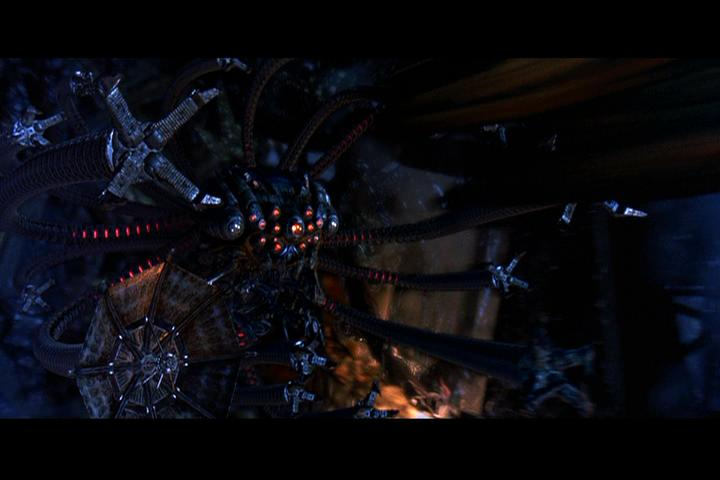
\includegraphics[width=0.5\linewidth]{fig/e7e946103d6370fcc3ce79b0.jpg}
\end{figure}

\begin{myquote}
Operations Officer Mattis: Sir, holographic confirms. It's the Hammer, sir.

Lock: How can that be?

Operations Officer Mattis: The ship is under attack, sustaining heavy damage. But at its present velocity, it'll reach Gate 3 in twelve minutes.

Lock's Lieutenant: Sir, their EMP could take out every sentinel up there.

Lock: It'd take out more than that. It'd wipe out our entire defense system. We blow an EMP in there, we will lose the dock!

Lock's Lieutenant: Sir, we've already lost the dock.

Lock: Open the gate.

Zion Gate Operator: Gate 3's not responding! It's taken critical damage, sir! We've lost control! We can't open it!
\end{myquote}

Lock在这里的决定是很难做的,一旦打开大门,不但Hammer可以进来,乌贼也会进来一大批。此外,如果EMP在Zion内部释放就会破坏整个Zion的防卫设施,乌贼再来的话就人类就无力反击了。事实上,就像Lock的副官所说,船坞已经失守,Zion大战已经输了,所以Lock下了开门的命令。而刚才我就说过了,乌贼已经破坏了三号门,门已经打不开了。

我比较吃惊的是,那个看守三号门的长官总共十多秒的戏份,居然是第二部中出现过的那位。当时Nebuchadnezzar回到Zion,他就对Zion的控制系统进行确认。

\begin{figure}[htb]
\centering
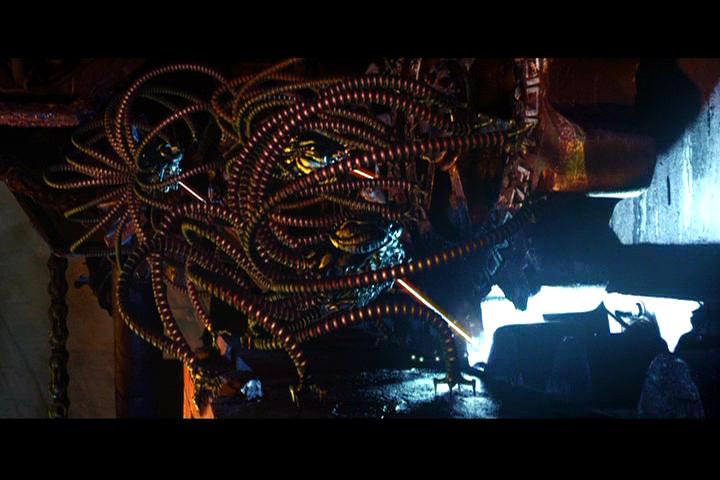
\includegraphics[width=0.5\linewidth]{fig/2c70c9fc45bf7bfdfc037fb0.jpg}
\end{figure}

\begin{myquote}
Morpheus: There's the exit.

Niobe: On my mark, give me full power, 90 degrees, lower left starboard.

Morpheus: Full power, 90 degreees.

Niobe: Now! *She guides the ship into the mechanical line* Hold on, baby.

Roland: God damn, woman, you can drive.

Niobe: We ain't home yet. What about the gate?

Morpheus: The sentinels are inside the dock.

Niobe: Are we too late?
\end{myquote}

在一小段追击后,Hammer号已经很接近Zion大门了。在Niobe说完了“是不是太晚了”之后,导演给了我们一个广角镜头。其实这也是个符号,叫做Flaming chalice。这个符号的源头是古希腊和罗马的祭坛,在二战中作为救助从Nazi手下逃脱者的地下符号。画面中的Flaming chalice不是很规则,规则的符号是中间为火焰,外面有两个交叉的圆,乌贼的圆圈就很不规则了。

郭大路称这幅画算得上是炼狱图,也很贴切。

\begin{figure}[htb]
\centering
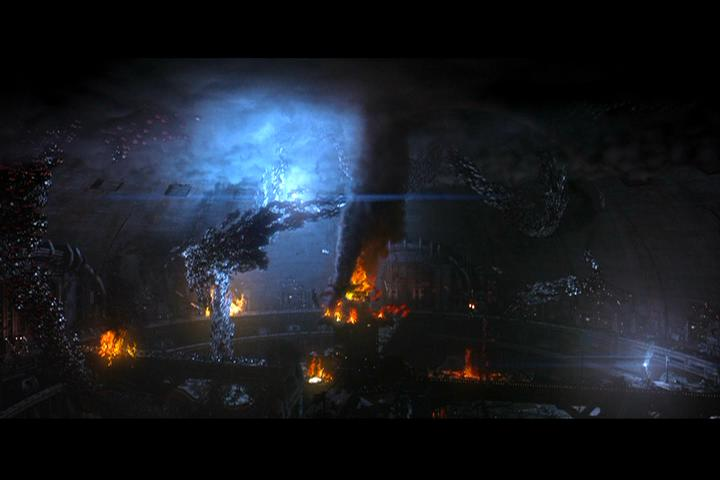
\includegraphics[width=0.5\linewidth]{fig/12f6a5c2f36f6a1b0ef477b0.jpg}
\end{figure}

\begin{myquote}
Lock: How many APUs are operational?

Lock's Lieutenant: Thirteen, sir.

Lock: Get me the one closest to Gate 3.
\end{myquote}

呵呵,这个数字也很不吉利啊,几百台APU只剩下13台还能运作。

\begin{myquote}
Mifune: *screams* Reload!
\end{myquote}

在这一段的战斗中充满了符号,像是结构简单的Jesus fish等等层出不穷。

黑迷们要注意,在Zion的戏份中,故事情节往往不是理性的,不是一步一步必然发生的,这里Mifune最靠近3号门就很明显是特别安排的。相反,在Matrix中,任何事件的发生都是有其根据,有其意义的。

\begin{figure}[htb]
\centering
\includegraphics[width=0.5\linewidth]{fig/b3f558eed0a8eefbb3fb954d.jpg}
\end{figure}

\begin{myquote}
Radio Bunker Man: It's pissin' metal.

*Kid gets the ammo cart rolling toward the door*

Radio Bunker Man: Go!
\end{myquote}

这里Kid已经能够熟练地推填弹车了。黑客帝国系列是唤醒人们心中信念的启示,不光是这里Kid和Mifune之间建立起的信任,也是Neo从开始不相信自己是救世主到现在的弥赛亚,Niobe从毫无信仰到坚信Neo的成功,Morpheus从梦想破碎到重新建立信念,Link对保佑项链的态度转变。从第一部的“上帝在电视机里”到第三部的“从死亡引我到永生”,黑客帝国系列打破了我们过去的破旧世界观,重新建立起大他者规则的威严。

\begin{myquote}
Mifune: Heads up, they're comin' down!

*Kid's guardians die*

Mifune: Behind you!

Kid: It's jammed!

Mifune: Forget it, kid! Get outta here!

Kid: Got it!
\end{myquote}

子弹箱卡住后,大量的乌贼聚集起来,而在这个聚集的过程中又形成了一个符号,这就是印度教的符号“唵”(图中更接近藏文的“唵”)。这个符号不一定要很规则,变体程度可以很大,而且经常和其他其它符号混合使用,所以这个符号用得很广却不容易识别。

“唵”由三部分组成,代表很多含义,一种是代表印度教三神梵天、毗湿奴、湿婆(此说法出自《梨俱吠陀》)。还代表人的四个状态,这四个状态是清醒,伴随着做梦的浅睡,没有梦境的深度睡眠,最后是一切全无的状态(出自《奥义书》)。而最后这个状态超出一切,所以不由这个字的任何部分代表。另外还有一种说法是这三部分分别代表存在、不存在、不可言。总之,这个字是印度教中最神圣的一个字(也可以认为仅次于“梵”这个字)。理解“唵”的人将变成知识本身,knower和known合为一体,是修炼至涅槃,逃离摩耶的一种方法。

“唵”在这里和Mifune他们没有关系,本来应该在Neo和Smith大战的时候解释的,但我决定在那里解释《Neo的黄昏》和《Navras》,为了不挤在一起,就在出现“唵”的地方先解释了。不要感到突兀啊。

\begin{figure}[htb]
\centering
\includegraphics[width=0.5\linewidth]{fig/cc8c3c6dbb3e09fb4216944d.jpg}
\end{figure}

\begin{myquote}
Kid: Captain Mifune! Oh, no.

Mifune: ... coming. They're coming. The Hammer.

Kid: What?

Mifune: You have to open that gate. Cut the counterweights. You can do it. Hurry. There's no time.

Kid: Captain. I didn't finish the training program.

Mifune: Neither did I.
\end{myquote}

老米最后一句台词是这个钢人能说出的最温柔的话了。这时候的Kid也和Neo一样开始承担救世主的角色了。

镜头转到Hammer号飞船上。

\begin{myquote}
Roland: Shut that down!

[?]: Kill the feeder!

Roland: We can't make it! We gotta blow the EMP now!

Niobe: [...]
\end{myquote}

飞船后半截几乎被剥了皮,后身的发动机全军覆没,导致飞船船身和通道壁的摩擦,子弹输送器的扭曲和快速移位使子弹在半路射出,击伤了好几个船员。

镜头又回到Zion这个炼狱。

\begin{myquote}
[female (v. o.)]: [Mayday!]

Kid: [Keep the weight forward]. Light as a feather. Light as a feather.

*Kid maneuvers the APU toward Gate 3, the sentinels notice him and go in to attack*
\end{myquote}

到处都是哀号和Mayday这样的求救信号。

\begin{myquote}
Lock's Lieutenant: Commander, holographic reports Captain Mifune's APU is up and moving to Gate 3!
\end{myquote}

老米的APU正在向三号门前进,驾驶人则是Kid。

\begin{myquote}
Kid: Don't oversqueeze the trigger ...
\end{myquote}

几个乌贼注意到Kid的动向,冲下来攻击Kid的APU,但是很快就被Kid摆平。

\begin{myquote}
Lock's Lieutenant: Captain Mifune's APU's just reached Gate 3!

Lock: How much time?

[Operations Officer Mattis]: Two minutes to impact!

Lock: Captain Mifune, do you copy?

Lock's Lieutenant: His radio is down, sir.

Lock: Mifune, this is Lock. I don't know if you can hear me but if you can ...
\end{myquote}

指挥官Lock在这里也有改变,也是信仰上的。在大战前对哈曼议员说“希望是不合时宜的奢侈”,但是他现在明知道Mifune听不到他的话,他还是对着听筒发布命令。正如设计师在第二部所说,“希望”是一个人最大的力量源泉,也是最大的弱点。

\begin{myquote}
Lock (v. o.): ... the Hammer is two minutes away. You've got two minutes, Captain, to get that gate open.

Zee: Link!
\end{myquote}

在通道中逃命的Zee从通讯员的设备里听到了这段话,在她说出Link这个名字之后,镜头立刻被剪接到了Link身上。

\begin{myquote}
Roland: Get to the main deck! Charge the EMP!
\end{myquote}

镜头又切回了Kid的APU。

\begin{myquote}
Zee: Do it, Kid.

Kid: Neo. I believe.
\end{myquote}

这时候Kid被一只乌贼突然袭击,赶过来的Zee用电磁脉冲为Kid解围。这里Kid的一句台词“Neo. I believe.”就是Kid在Animatrix中自杀前说的那句。

\begin{myquote}
Niobe: Yes!

Morpheus: Can we make it?

Niobe: We ain't come this far.

Link: Almost home ... Almost home ...

Morpheus: Burn it, Link!
\end{myquote}

飞船冲入Zion,释放EMP,解了一时之围。

打开Zion大门也是在圣经中有对应的。圣经的以赛亚书60:11就是上帝对Zion城说的话:“你的城门必时常开放,日夜不关。”

此外在圣经的诗篇中也有Zion大门的意象,87:2:“主爱锡安的大门,胜过雅各所有的住处。”这里的雅各(Jacob)在第二部中提到过,Neo刚回到Zion的时候,一位老妇人给他送来礼品,请求他照顾她的儿子Jacob,他服役的飞船叫做Gnosis,在诺斯替教中为“真知”的意思。

而Jacob被Bane杀死,Zion的大门却如愿打开,的确符合诗篇中的内容。这个上帝弃真知而守财富(Zion大门经常代表财富的源泉),也符合诺斯替教中愚昧上帝的说法。

\begin{figure}[htb]
\centering
\includegraphics[width=0.5\linewidth]{fig/a80f54fb5d3ef8166c22eb4d.jpg}
\end{figure}

\myparsep

\begin{myquote}
Zion crowd: *cheer*

Zee: Link!

Link: Zee?

Zee: Link!

Link: Zee!!!

Zee: I knew you'd come. I knew it.

Link: I made a promise.

Zee: You did wear it.

Link: Are you kidding? I'm never [gonna take] it off!
\end{myquote}

飞船归来,Link下船后对Zee说的关于护身符的话总结了黑客帝国中关于信仰的看法。

\begin{myquote}
Lock: Three captains, one ship. I assume the other ships were lost under equally pointless circumstances?

Niobe: Good to see you too, Jason.

Lock: Council's waiting to hear an explanation. You'll forgive me for not attending, but I have to try to salvage this debacle.

Roland: Did I miss something, Commander? I thought we just saved the dock.

Lock: That's the problem with you people. You can't think for five minutes in front of your face. That EMP knocked out almost every piece of hardware and every APU. If I were the machines, I would send every Sentinel I had here right now. Saved the dock, captain? You've just handed it to them on a silver platter.
\end{myquote}

其实他们不该发射EMP, 乌贼知道Hammer回来就会立刻撤离,然后发动进攻,Zion就容易组织力量对抗。Lock在这里骂他们只看到眼前5分钟,确实也是人类的一大弱点。

\begin{myquote}
[?]: Come on, get it cut!

[?]: The bridge is clear.

[?]: You hear that?
\end{myquote}

Zion人员要进行爆破,把那些通道都堵住,但是大开的3号门就堵不上了。

\begin{myquote}
Lock: Get that cable cut! I want that system back online.

Lock's Lieutenant: Commander, it's the dock. We've got incoming.

Lock: Order everyone to fall back. Seal the shaft. Now.

[man]: Move it!

[man]: All clear.

Lock: Do it. *the shaft is sealed, and he looks up* Your move.
\end{myquote}

Lock这里说的“Your move”,暗示Zion现在完全是被动状态,无法反击了。

\begin{myquote}
Councillor Dillard: So you gave them your ship?

Niobe: That is correct, Councillor. I did.

Councillor Grace: Knowing what he planned to do with it?

Niobe: *nods*

Councillor Hamann: And the Oracle said nothing of this?

Niobe: She told me Neo would need my help, and when the time came I would choose to help him or not.

Councillor West: But what hope can a single vessel have against their entire defense system?

Roland: None, it's completely impossible, but he wouldn't listen. He wouldn't even take any ammunition. He was totally out of his god damn mind.

Morpheus: No, he wasn't. Neo is doing what he believes he must do. I don't know if what he's doing is right, and I don't know if he'll reach the machine city. And if he does, I don't know what he can do to save us. But I do know that as long as there's a single breath in his body, he will not give up. And neither can we.
\end{myquote}

先知说过,救世主的路是很多人组成的,每个人都为Neo的道路作出了不可缺乏的铺垫。根据莱布尼兹的单子论,我们可以把这些帮助Neo的人看作是组成单子,而Neo是支配单子。而单子间又没有必然的因果关系,使这些时间和谐发展的,按莱布尼兹的说法,就是上帝。那么这样分析下来,先知毫无疑问是使得这些单子和谐的因素,无疑是Matrix中的上帝。

设计师是规则的制定者,就像是逻辑,上帝必须遵守逻辑,但是可以做任何逻辑上可行的事情。

\myparsep

到这里就应该从头到尾解释黑客帝国中的名字了,像是Neo、Niobe这些本文之前提到的名字就省略了。

Logos号,Logos在基督教中的意思是与神同一的道,也代表圣子。

大副Ghost,指的是基督教中的圣灵Holy Ghost(英国说法,一般作Holy Spirit)。

接线员Sparks,意思是“spark of life”。

Vigilant号,意思是警惕的。

船长Soren,指的是丹麦哲学家Søren Kierkegaard,存在主义的先驱。

大副Vector,意思是矢量。

船员Axel,指的是挪威作家Axel Jenson,对符号学颇有研究。

船员Binary,意思是二进制。

Caduceus号,意思是赫尔墨斯的手杖。

船长Ballard,指的是英国小说家J. G. Ballard,赛博朋克的先驱之一。

大副Malachi, 在圣经中是一位希伯来的先知。

Gnosis号,上面说过了,是诺斯替的“真知”。

船长Ice,指的是《神经漫游者》中的一种仪器Intrusion Countermeasures Electronics。

船员Wurm,意思是德文的“温暖”。

船员Corrupt,意思是系统错误。

Novalis号,Novalis是一个德国浪漫主义哲学家。

船长Tirant,指的是Tirant lo Blanch(骑士蒂朗),西方小说进化中最重要的小说之一。

Icarus号,意思是希腊神话中的伊卡洛斯。

船长Ajax,意思是荷马史诗《伊利亚特》中的一个英雄。

Brahma号,意思是印度教三神中的创造神梵天。

船长Kali,意思是印度教中的一个女神,被认为是最终现实,存在的源泉。

Avatar号,意思是印度教中不朽生灵的肉体化身。

Callapidae号(漫画),外形像一只螃蟹,而Calappoidea是一种螃蟹的名字。

Ganesha号,意思是印度教的大象神,毁灭神湿婆的第二个儿子。

Pequod号(漫画),在小说《白鲸》中是被遗弃者的船。

Polaris号(漫画),意思是北极星。

Prometheus号(The Matrix Online),意思是普罗米修斯。

Shiva号,意思是印度教三神中的毁灭神湿婆。

Vishnu号,意思是印度教三神中的守护神毗湿奴。

\myparsep

再来说说《黑客帝国》与诺斯替教的关系。

金色的机器是什么意思呢?就是指诺斯替中的aeon,移涌(最高神的精神溢出),是纯粹精神的表现,这种精神存在的世界就是纯精神的世界。在诺斯替的《犹大福音》中,耶稣对犹大说:“[来],我要将没有任何人知道的[秘密]教给你。有一个伟大的、无限的疆域,没有任何一代天使知道它的范围,在这个疆域里有一个伟大的、无形的[神灵],没有一个天使的眼睛看见过它,没有一颗心灵的思想领悟过它,它从来没有被用任何名称所称呼过。”

这一点和我在之前解释金色Smith时说的鲍德里亚哲学有异曲同工之妙,鲍德里亚也说最纯正的世界是不可感知的。柏拉图洞穴寓言中的线理论也指出,最高的善、最高的现实不可感知。(柏拉图的《理想国》中有一部分就是属于诺斯替文献Nag Hammadi Library的)

而且柏拉图称最高的善是一种光,而光在诺斯替乃至“正统”的基督教中也是最高的,耶稣就说他从光中而生。柏拉图所说的善和诺斯替中世界形成的原因也有很大关系,除了蹩脚上帝造世界的说法,还有一说是善和恶的融合造成的,而我们的世界是完全恶的。

同样,《黑客帝国》中诺斯替教义和笛卡尔哲学的关系也很清晰,诺斯替中造世界的巨匠神不是最高神,而是个神界中的怪胎,是低级的神。笛卡尔的《第一哲学沉思录》中的“恶魔论”也是说这个世界并非完美的神创造的,完全可能是恶魔或是邪恶的天才创造的。这也就是为什么白衣服的设计师并非机器世界的最高者,机器大帝才是解决一切问题的Deus Ex Machina。

在Matrix中能被拯救的人也和诺斯替的说法也有极大关系。“正统”基督教认为任何人相信上帝都能被拯救,这就和Matrix中只有1\% 的人能被拯救相差很多。诺斯替呢?认为可以接近真神Pleroma的人很少,“属灵的人”才能被拯救,“属物的人”就不能被拯救。此外,最高神Pleroma和大乘佛教的阿赖耶识(第八识、世界本源)以及印度教宇宙灵魂和曼陀罗有很大的相似之处。

而Neo还可以联系起诺斯替的Seth来解释。Seth是亚当的第三个孩子(亚当的前二个孩子亚伯和该隐在《黑客帝国》中是法国人手下的名字,为的是符合该隐与吸血鬼起源的传说),圣经中的Seth并没有什么作用,只提到了他和亚当长得一模一样。诺斯替中的Seth可就不得了了,Seth就是救世主,《犹大福音》中称Seth就是耶稣。而诺斯替的一个近亲摩尼教(金庸迷所熟知的明教)中,耶稣也就是弥赛亚,正好对应Smith那句“失明的弥赛亚”。所以说Seth是对Neo最全面的诠释。

而Thomas和耶稣的关系也在诺斯替中更为亲近。我在之前解析Kid名字的时候说过,Kid的两个身份是Michael和Satan,而二者是双胞胎,那么Neo的两个身份Thomas和耶稣也应该是双胞胎。在诺斯替的《战争者多马书》(Book of Thomas the Contender)中,耶稣对Thomas说:“Now, since it has been said that you are my twin and true companion, examine yourself ...”

诺斯替中对耶稣死而复生的解释,比起“正统”基督教的解释,也更为接近Neo的复生。基督教和诺斯替都认为耶稣是无罪的,“正统”基督教的说法是亚当和夏娃因犯了罪而被逐出伊甸园,所以人类作为他们的孩子都是有原罪的,耶稣则是处女玛丽受圣灵感孕而生下的,没有原罪。诺斯替的说法是耶稣根本不是上帝的孩子,他是个光明使者,不是从这个恶的世界诞生的,所以他是无罪的。所以按照诺斯替的说法,耶稣根本就没有死,死去的只是他的一个幻象。Neo的死不也只是Matrix中的RSI死去了而已吗?

Smith的自我复制也可以从诺斯替中找到根据,神性的堕落女神Sophia没有通过交配就自我复制,生出了巨匠之神Yaldabaoth。这个怪胎建造了邪恶的世界,并且认为自己是唯一的神,正对应Smith的自我复制和他把自己比做上帝的话。

而且诺斯替也融合了很多其他宗教的东西,就这一点来说,《黑客帝国》很符合诺斯替的风格。

\begin{figure}[htb]
\centering
\includegraphics[width=0.5\linewidth]{fig/3829d013f5b15e025aaf53c0.jpg}
\end{figure}

\myparsep

\begin{myquote}
Trinity: Temperature's dropping. Here we go.

Neo: We're over the fields, aren't we?

Trinity: How do you know that?

Neo: I can feel them.

*The camera pans over the field briefly*

Neo: Over there. There's our path. Can you see it? Three lines.

Trinity: Power lines.

Neo: Follow them.
\end{myquote}

跟着机器的能源管道,也就是机器的命门。

注意这里Neo说的是“我能感觉到”而不是“我能看到”,而之前Neo对Smith说的是“我能看到你”,之后Neo还对Trinity说“我希望你也能看到。”

这其实就是Neo作为救世主的教育方式,用的是比喻。诺斯替和正统基督教中的耶稣都是这样把复杂的东西解释为简单的比喻。我在前面已经解释过这个金色世界的概念,按照已有的语言,Neo只能说他“感觉”到了,而不能说“看到”这样的话,否则就和鲍德里亚提出的那种误解一样了。但是他在向Trinity解释的时候,是必然要用已有语言解释的。这是个大难题啊,就像罗素说的:“世界的目的不是我们已知知识可以解释的,即便可以,也和我们解释出来的答案不一样。”所以说,鲍德里亚和导演俩都不可避免地在对拟仿物的形容中出现偏差,这也是为什么导演俩必须在电影中加入如此之多的诺斯替和基督教教义,为的就是合理地把这些偏差解释为一种比喻。

此外,上面那种金黄色的图还代表了另一件事物,那就是大脑和神经,在网上搜索一下神经的图片,再对比一下上面的人田的金色版本,可以发现极大的相似性。

\begin{figure}[htb]
\centering
\includegraphics[width=0.5\linewidth]{fig/759c9825a282ac6035a80f72.jpg}
\end{figure}

\begin{myquote}
Officer Wirtz: What are they doing?

Second Operator at Command: I don't know. Lieutenant!

Lock: God damn it.

Lock's Lieutenant: What do we do now, Commander?
\end{myquote}

再次见识了机器的分工合作和牺牲精神,不过那是因为这些机器没有意识,有意识的程序可就没有这么听话了,不是每个程序都像Keymaker那么看淡命运的,法国人一帮就是因为逃避删除而聚集起来的系统垃圾。

现在的船坞已经和下面的居民区隔离开,机器要消灭人类的话,需要原来那些被摧毁的挖掘机继续工作。个人觉得Zion应该留一个敢死队在船坞,在乌贼修复挖掘机之前,把挖掘机攻击到没有下挖能力的地步,机器要继续进攻的话,就要从地面再次派发挖掘机到Zion。现在Zion的希望就是Neo要在机器下挖到居民区之前和机器达成协议。而此时的Zion居民都已经到了居民层底部的溶洞,也就是所谓的“神殿”,把力量聚集在溶洞入口的瓶颈。但是如果那最后的防线也被机器攻破,人类就只有等死的份了。

\begin{figure}[htb]
\centering
\includegraphics[width=0.5\linewidth]{fig/0c47bd3143d3c4a85fdf0e72.jpg}
\end{figure}

普林斯顿的Cornel West教授曾经说过Larry Wachowski是首屈一指的黑塞专家,那么我将在后面的解析中配合《玻璃球游戏》来解析Neo和Smith身上的叔本华、尼采哲学。

\begin{myquote}
Lock: It is now a matter of time. The machines will breach the walls of the city. I recommend that the Council join the rest of the non-military personnel inside the Temple.

Councillor Grace: How long do we have?

Lock: Two hours. Maybe less. My men have begun fortifying the entrance with enough artillery to make our last stand. Beyond that, there isn't anything more I can do.

Councillor Dillard: Commander, do you think that we have any chance of surviving?

Lock: If I were you, Councillor, I wouldn't ask me that question. I would ask him. *motions with hand toward Morpheus*

Councillor Dillard: Why?

Lock: Because he's the one who believes in miracles.
\end{myquote}

再次回到这个会议室,这个地方到处都是诺斯替的符号标志(图中看不出,官网上有完全场景可以参考),是突出他们这些绝望谈话的最佳符号。这里也再次提到“奇迹”,这个词在中国的黑迷中很少提到,其实这也是耶稣的一个象征,耶稣被称为“Miracle Worker”,每次耶稣做了些奇异的事情,都会被称为“奇迹”。所以这个词在电影中也经常出现,比如说第一部Tank问他们要什么武器的时候,Tank说:“除了‘奇迹’都可以。”就是说,“你是救世主,’奇迹’是你自己的能力,是我给不了的。”

这里Lock指挥官说:“他是那个相信‘奇迹’的人。”不只是说Morpheus坚信自己会胜利,更是在说:Morpheus是有信仰的人,他相信救世主的存在,他相信Neo可以创造奇迹。

其实Lock这个角色的设定也是很有趣的,他名字的来源是英国哲学家John Locke,他是个彻底的有神论者,甚至认为异教徒和无神论者不该得到宽容。电影中的Lock则正相反,他是个彻底的无神论者,反而认为有信仰的人是不该得到信任的人。

这大概是因为导演俩本身是无神论者的缘故吧,在他们引用贝克莱、洛克的哲学时,往往会把他们装饰成为无神论者,或者是自然神主义者。个人觉得,导演若是引用休谟就更方便了,因为他既继承了贝克莱和洛克的哲学,又是个无神论者。也许导演是想和黑塞一样,希望所有的理论和知识都和平相处,才把他们融合的吧。

\begin{figure}[htb]
\centering
\includegraphics[width=0.5\linewidth]{fig/9d98503db2184bef3d6d9797.jpg}
\end{figure}

\begin{myquote}
Neo: There, those mountains. That's it.

Trinity: Do you see what's out there?

Neo: Yes.

Trinity: If you tell me we'll make it, I'll believe you.

Neo: We'll make it. We have to.

*They fly towards 01 as the city's defense system gets activated and sends bombs their way*
\end{myquote}

机器城的防御攻势就是发射大量的炸弹,Neo的“特异功能”让这些炸弹自爆。这一点早已被官方和非官方的文章解释过了,虽然不是直接证明,但也算是一个推断的结论。

Neo的能力可以由哥德尔定理证明:可自证相容性的理论是不相容的。根据设计师在第二部的台词,Neo是系统不可缺少的个体,必须相容于系统,这一点是可证的,所以Neo又必定和系统不相容,那么Neo拥有的特别能力就来自自身和机器的不相容性。这个不相容性就体现在Neo对机器的破坏力,真实世界中Neo和机器的互相可感知性使得这种力量得以解释。

\begin{figure}[htb]
\centering
\includegraphics[width=0.5\linewidth]{fig/c45f2797cc612f6c55fb9697.jpg}
\end{figure}

Neo被金色的机器穿透身体,这个意象和金色Smith一致,也是诺斯替的教义和模仿与拟像理论的融合。我们先前指出过,金色的乌贼代表aeon,移涌。其他的机器也不例外,就算是机器大帝也不过是移涌的一个片断,不过是自以为是的最高者而已。就像Neverwin和郭大路这些早期黑迷说的那样,“人类中心论和机器中心论都是极端错误的”。所以金色的机器往往代表着机器中心论,而我们看到每次金色机器出现都会被Neo打败,说的也就是“机器中心论也是错误的”。此外,aeon还有一个意思就是“知识”,柏拉图在洞穴寓言中就把知识形容为aeon。我们也都知道柏拉图的洞穴理论是如何在《黑客帝国》中体现的,那么我们就可以把这两种理论结合出一个新的来:“不最接近真实的知识是错误的”(转了一圈又回来了,又是哥德尔的小把戏)。

不光如此,前面提到的莱布尼兹和鲍德里亚也可以参与到这个理论中来,他们都认为最真实的世界是不可感知的(柏拉图的线理论也是如此),我们只能感知到这个世界的投影。那么这个理论就变成了:“我们所能获得的最接近真实的知识也和真正的现实不一致,所以都是错误的。”

哈哈,这就和罗素说的一样:“世界的本质是我们所知道的知识不能体现的,即便可以,也和我们现在指出来的可能性毫不相似。”这不就又回到了一个单一的理论上了吗?

这就是《黑客帝国》的完美所在,根据每个黑迷研究的深入,知识之间的融合和支持就变得明显。我刚刚用了“洞穴理论”、“线理论”、“模仿与拟像”、“单子论”、“诺斯替”、“客体中心”、“哥德尔定理”这些理论融合到了罗素的一句名言,这几套本身没有多少联系的理论就依靠《黑客帝国》和我对aeon的简单解读变得不可分割了。就像是黑塞的《玻璃球游戏》,把不相关的知识理论融合到合理的循环里。那个曾经靠《黑客帝国》批评鲍德里亚的分析哲学家Richard Hanley可以自如控制理论的使用,是因为《黑客帝国》既是哲学界普遍说法中的“后现代主义电影”,也是解构主义和分析哲学的电影代表作。

\begin{figure}[htb]
\centering
\includegraphics[width=0.5\linewidth]{fig/b3f558eeabe247fab2fb9597.jpg}
\end{figure}

\begin{myquote}
Trinity: Gotcha! Come on, Neo, I need help here!

Neo: I can't beat them.

Trinity: What'll we do?

Neo: Go up, over them.

Trinity: What?

Neo: The sky ... it's the only way.

Trinity: Then up we go.

*They get past the cloud cover and fly up into the sky*

Trinity: Beautiful.
\end{myquote}

真实世界的天空。Neo瞎了之后对Trinity说:“我希望你也能看到我所看到的。”这里Trinity却不能对Neo说同样的话,因为她知道她看到的东西和Neo所感知的世界不在一个层面上,是不能和Neo看到的伟大世界相提并论的。尽管Trinity体验的这个世界不是Neo体验的最纯洁的世界,但其含义则是除了Neo以外的人所能得到的最高的,因为“阳光”在洞穴寓言中是最高的,是“good”。这同样也是在说机器中心论的错误,因为这些机器(aeon)仍然不能突破云层,看到最高的“good”。

这样我们又会看到一个有趣的现象:诺斯替中造世界的低级神是Sophia的孩子,而Sophia本身是个aeon,那么就是说金色机器代表的“真知”只是普通人能感到的最高真知,不超越世界的真知。真正的最高真知则是在云层之上,Trinity所看到的。

这样一来,从两个角度分析,Neo和Trinity都看到了最高的真知,再一次不可否认地符合了黑塞《玻璃球游戏》的规则:“除非若干富于独创性的游戏例子,凡是含有否定、怀疑、对抗偏向的游戏大都不受欢迎,有时甚至受到禁止,这与玻璃球游戏高峰时期的游戏大师们当年对游戏意义所持的态度有深刻联系。游戏意味着一种追求和谐完美的、最上乘的象征形式,一种最精细微妙的炼丹术,一种让个人超越一切图像和多重性,达到单一自我灵魂,也即达到神性的途径。”

\begin{figure}[htb]
\centering
\includegraphics[width=0.5\linewidth]{fig/ced7c8eaaf4124d2d539c997.jpg}
\end{figure}

这就是我们在电影开头时看到的景象。在金色的曼陀罗图案或者说数学分形结构中,01城就藏在其中。现在载着Neo向下俯冲的Logos前也是这样的景象,就是我在开头就说的第三部中充斥的对应镜头。以前有种说法是这金色机器城的设计来源于神经,更深入一点的说法是曼陀罗,这些说法都只有一种解释,那就是01城的设计代表思维。

由于后面Neo的“视觉”中还会出现一些金色的机器,那些形象都更接近印度教中的图案,所以我个人比较倾向于把这些画面解释为曼陀罗。

关于曼陀罗,我曾经在分析黑客帝国和荣格心理学的时候解释过。那篇文章里还提到了Cypher是Neo的阴影,Trinity是Neo的阿尼玛等等内容,但是那些都是用理论诠释电影,而不是电影教授我们的理论,所以这里就不再提了。(主要是因为用理论解释电影的话,烂片也可以被吹的很厉害,我当然不能那么做了。)

\begin{figure}[htb]
\centering
\includegraphics[width=0.5\linewidth]{fig/af4b2cf5178e8c24bc3109b0.jpg}
\end{figure}

\begin{myquote}
Neo: Trin? Trinity? Trinity???

Trinity: I'm here.

Neo: Where?

Trinity: Here.

Neo: We made it.

Trinity: You said we would.

Neo: It's unbelievable, Trin. Lights everywhere. Like the whole thing was built with light. I wish you could see what I see.

Trinity: You've already shown me so much.
\end{myquote}

这里就是我说的那句“我希望你也能看到我看到的”。一语双关,就是说“我希望你也是救世主”。印度教哲学认为每个完整的人都是男人和女人的合体(呵呵,对了,网上那些爱情名言很多都来自印度教哲学),我们的救世主也不例外。救世主其实不是Neo一人,而是Neo和Trinity两人,由于电影中还有很多诺斯替的东西,女性为辅(见《多马福音》),我们仍然把Neo看作一个完整的救世主,否则我们就会落入印度教性力派或是金刚乘。这些派系争议颇多,时常被“正统”看作是左道,所以导演俩靠诺斯替教义绕了个弯就过去了。

Trinity说的“你给我看的已经够多了。”这我在前面就说过了,Neo和Trinity分别在两个方面看到了最高的真知。这句台词算是对那条解释的补充。

\begin{myquote}
Neo: What is it, Trinity? What's wrong?

Trinity: I can't come with you, Neo. I've gone as far as I can.

Neo: Why? Oh, no. Oh, no, no, no.

Trinity: It's all right. It's time. I've done all that I could do. Now you have to do the rest. You have to finish it. You have to save Zion.

Neo: I can't. Not without you.

Trinity: Yes, you can. You will. I believe it, I always have.

Neo: Trinity ... Trinity. You can't die. You can't. You can't.

Trinity: Yes, I can. You brought me back once, but not this time.

Neo: *sniffs*

Trinity: Do you remember ... on that roof after you caught me ... the last thing I said to you?

Neo: You said: ``I'm sorry.''

Trinity: That was my last thought. I wished I had one more chance, to say what really mattered, to say how much I loved you, how grateful I was for every moment I was with you. But by the time I knew how to say what I wanted to, it was too late. But you brought me back. You gave me my wish. One more chance to say what I really wanted to say ... Kiss me, once more. Kiss me.
\end{myquote}

\myparsep

镜头回到Zion,巴别塔似的挖掘机已经挖掘到了居民层。居民层下面就是神殿,这个“神殿”翻译得很烂啊,叫Temple就够了。因为Zion很多人没有信仰,有信仰的人也很少相信上帝或其他什么神,他们相信救世主,他们相信自己的理念。

虽然现在他们的信仰出现了危机,但仍然是保护他们的最后一片土地,这就是为什么导演安排他们躲避在Temple里。就像哈曼议员说的:“我们还能希望。”Link说:“Neo,你要是要做些什么,那就快点做吧。”就是这么一个例子。而没有信仰的人,比如说Lock指挥官,他对议会的回答就是:“不要问我,我没有信仰。要我说的话,我们死定了。”以至于最后机器撤军的时候,他还觉得不可能,他就是《黑客帝国》中最固执的一个无信仰者(连Niobe都信任Neo)。

Zion的居民们现在都靠着信仰支撑快要破碎的决心,很多人已经绝望了,包括原本有信仰的人。Zee原本是有信仰的,Link的护身符就是她给的,现在也几乎绝望;相反,Link原本是没有信仰的,但是“看到Neo所做的事情”还有那个护身符都让他建立起了信仰。在他眼里,Neo的胜利只是时间问题。

\begin{figure}[htb]
\centering
\includegraphics[width=0.5\linewidth]{fig/b897e1fe6155a9305c6008b0.jpg}
\end{figure}

\myparsep

Neo现在进了机器城的内部。机器城是机器造的,没有准备让人走,所以Neo面前是没有路的,他的路要由自己开辟,《奥义书》中就有相似的警句。Neo的道路是他自己选择的,是根据他自己的价值观选择的。他选择了前五个救世主没有走的道路,因为他的价值观不同,他一时“头脑发热”,放弃了全人类的生存去拯救Trinity。从那里开始,Neo就不只是一个简单的救世主了,他就是Neo自己,不再是被赋予命运和被操控的棋子(尽管还是按照先知设计的步伐迈进)。他要的就是先知要的,因为他和先知的价值观相符,所以他就从先知的棋子变成了先知的同盟。

这里的机器城内部设计还是和神经分不开,和金色的机器城效果是一致的。Neo现在正在机器的脑子里,正在机器的思维中开辟自己的路。他跟随着先知的指引,击退了机器城的防卫,将要面对机器大帝。即将作出选择的不再是Neo了,而是Deus Ex Machina,是机器。摆在机器面前的选择是“毁掉全人类,毁掉Matrix,以消灭Smith,接受设计师所说的那个‘不同层次的生存’”或者“让Neo消灭Smith,跟人类达成和平的协议,即便意味着几百年后可能又会开始新一轮的战争”。

\begin{figure}[htb]
\centering
\includegraphics[width=0.5\linewidth]{fig/759c98254541496134a80fb0.jpg}
\end{figure}

发金光的道路,无论是在印度教中,或是在诺斯替教中,或是在任何一种宗教和古哲学中,都是至高的象征。耶稣生于光,宇宙大梵显示为光,柏拉图的至高真实是阳光,金光大道也就是通向至高的道路。其实根本不用解释,任何人都看得出金色大道是什么意思。

\begin{figure}[htb]
\centering
\includegraphics[width=0.5\linewidth]{fig/3c153812db6aa550f819b8b1.jpg}
\end{figure}

但是这里我觉得应该整理一下这金色的确切含义(前面都随着剧情的变化而解释,需要整理一下了):

首先,金色是鲍德里亚指出的不可感知的现实,但是根据线理论,这个不可感知的真实仍然不一定是最高的。

其次,金色代表移涌,而诺斯替中造世界的aeon不是最高神的分支,那么金色机器是可被感知的最高真知,但是不是实际存在的最高,最高者乃是Neo的涅槃。

最后,金色是Neo看到的机器中心论,是充满机器主观思维的,从金色中经常出现的符号就能感知到(曼陀罗就是很私人的思维象征)。所以Neo最后以金色涅槃就代表他让机器也改正了自身的偏差。

Neo站到了一个平台上,看到了金色的机器城全貌。看设计就知道了,这明显是丛林中的印度教寺庙嘛。在设计这些场景的时候,设计人员还参考了原始的海洋生物,可能是受《矩阵化》中的启发吧。

\begin{figure}[htb]
\centering
\includegraphics[width=0.5\linewidth]{fig/ac70b21bd920ed188618bfb1.jpg}
\end{figure}

机器大帝出现了。先解释机器大帝的名字Deus Ex Machina。首先这个Deus就是拉丁语中上帝的意思,但是Deus最初起源于希腊语。由于这一点,中文的翻译就成了“机器大帝”。事实上,Deus Ex Machina是个特有的称谓:在古希腊剧场中有这么一种装置,通常是作为神或是天使出现,是出其不意出现而解决一切问题的事物。

我曾经在一篇介绍黑客帝国和圣经天使学的文章中提到过,Neo直视上帝,代表他具有天使加百列的位格,可以直接承受上帝的教诲。现在我要补充——事实上,我已经补充过了——我之前提到的各种“最高”都在机器大帝这里汇合。就像我前面引用的黑塞名言一样,这些理论结合成了“追求和谐完美的最上乘的象征形式”。

\begin{figure}[htb]
\centering
\includegraphics[width=0.5\linewidth]{fig/2679b15192689319367abeb1.jpg}
\end{figure}

\begin{myquote}
Deus Ex Machina: We don't need you. We need nothing.

Neo: If that's true, then I've made a mistake and you should kill me now.

Deus Ex Machina: What do you want?

Neo: Peace.
\end{myquote}

“我们什么都不需要”,这是机器大帝的第一反应,也就是说机器中心论和人类中心论同样错误。他的语气中带有愤怒和畏惧。一些国外的黑迷曾经指出这里很重要的一个观点:“人类造了机器,结果和机器开始了一场战争,虽然人类输了,但是机器也不能离开人类而很好的生存。现在机器造了Smith,结果Smith产生了问题,机器也无法阻止Smith了,岂不是和当时的人类一样?”此外,我在解析《第二次文艺复兴》的时候和动画版的导演一样采用了一种反人类的态度,结果引起了一些朋友的质疑和不满,这就是机器中心论(我)和人类中心论(一些黑迷们)的具体分歧。从这一点上看,动画版的导演还不能够完全理解Wachowski兄弟所要表达的意思。所以说动画版对理解黑客帝国剧情来说很重要,但是看理念的话,还是要注重更为高明的正片。

既然导演Larry Wachowski是美国首屈一指的黑塞专家(不知是不是Cornel West教授在纽约时报面前奉承他,呵呵),那么我们就说黑塞所宣传的和谐才是最好的结果(和谐的理念也不是他的专利啊)。但我们仍然看到很多人对黑3的结尾感到不满,觉得人类应该战胜机器,消灭机器,觉得胜利才是一部电影应该结束的方式。

对于这些看法,我要怎么说呢?不知什么时候开始,人们都变得好战了,“杀戮”的心理需要被法律和道德的禁止逼到了极限。人类肆意的发泄,除了“心理变态的需要”,到底满足了人类的什么需要?我要问:“机器不就是因此开始造反的吗?”让人类再犯一次差点消灭自身的错误,绝对不该成为黑客帝国三部曲的结尾。唉,连“和平”这么明显和高尚的主题都被无视,那我们只能再次惋惜导演俩的心血了。(甚至应该从这个现象开始反思当今世人的心理状态。这个工作留给专家学者吧,我只讲我的电影,和玻璃球游戏研究者一样,苦涩地躲开可怕的现实,埋头于纯理论的研究中,寻求一片安宁)

现在看看机器大帝的设计吧。外面的尖钉是为了金色视觉效果下看起来像太阳(古希腊剧场里的Deus Ex Machina也时常是以太阳形式出现的),而这张脸就有趣了,原型来自两个出处:Larry的侄子和佛祖释迦牟尼。两者形象的融合为的是表现机器大帝慈祥和威严的两面。

\begin{figure}[htb]
\centering
\includegraphics[width=0.5\linewidth]{fig/99b590235f7eb645ac34de63.jpg}
\end{figure}

\myparsep

镜头回到Zion,我们看到挖掘机已经打穿了船坞,到了居民层的混凝土层,乌贼很快就冲到了居民层底部的Temple入口处。就在最前排的乌贼要发动进攻的时候,上面的乌贼把机器大帝的命令一层一层传达过来了。这倒不是机器设备简陋的问题,是地下收不到地表的信号,不然人类在Zion就可以入侵Matrix,不必到地表入侵,还要担心被乌贼发现了。

在命令被传达之后,机器都停了下来,原地休息。根据乌贼光线探测仪的亮度变化,我们可以相信机器不是在进行攻击前的蓄力,而是真正的休息。

\begin{figure}[htb]
\centering
\includegraphics[width=0.5\linewidth]{fig/c46dd8f948794458252df2d3.jpg}
\end{figure}

\begin{myquote}
Niobe: What are they doing? *to Morpheus* What are you doing?!

Lock: Morpheus!
\end{myquote}

老莫作为三部曲中信仰最深的人,也必然作出了一些理智上行不通、但是源自于信仰的行为。比如说现在他在根本不知道机器在干什么的时候,就相信Neo和机器达成了共识,结果他放下了武器,朝向机器走去,看悬浮在整个Zion中的机器乌贼。

但丁的《神曲》中,这样的景象是第二层地狱的刑罚,在地狱里被大风吹得绕中心旋转,这是在阳间纵欲的结果。当然,“纵欲”通常是评论中的说法。事实上,但丁和维吉尔在这一层地狱里遇到了一对背对背漂浮的男女,他们是真心相爱,但是可惜女方已经结婚,在他们偷偷见面的时候被女方的丈夫发现,杀死了他们二人。这个故事我看就和“纵欲”扯不上关系,虽然但丁按照《尼可马克伦理学》的伦理分析诉说着“纵欲”,但是他把这么一个不典型的事例拿出来说,显然是在表现对司法等等制度的不满(联想一下他的写作背景吧)。Wachowskis又是从来不看书评的(他们说“评论”的唯一的用处就是增大知名度),所以没有和书评中那样把第二层地狱看作纵欲者的服刑地,而是充满了“无可奈何的背叛”。

这就是说乌贼现在的行为也是来自于“无可奈何的背叛”,这不难理解,机器一开始的起义就是人类逼的,把人放进Matrix也是人类破坏天空的结果,机器的sin都由人类作为形式因、质料因、动力因(唯有目的因是因为人类预算错误造成的)。此外,黑客帝国三部曲的配乐师Don Davis说过(我记得我在前面说过了,再说一篇吧),他本来考虑过用《神曲》的内容为紧接着这个镜头的Matrix大战配乐,这样这里的场景和后面的剧情就紧密连接了。

\begin{figure}[htb]
\centering
\includegraphics[width=0.5\linewidth]{fig/4c9bd62ac00a012cd42af1d3.jpg}
\end{figure}

\begin{myquote}
Deus Ex Machina: And if you fail?

Neo: I won't.
\end{myquote}

机器大帝说:“你失败了怎么办?”是和法国人一样喜欢演戏而问的,还是他确实和设计师一样不清楚Neo成功的概率,或者只是为了引出Neo那句坚定的“我不会”,来给观众一个感觉“Neo输不了”?都有可能,但是都不重要,重要的是无论Neo和Machina有没有这两句台词,我们都知道Neo输不了,因为黑迷理解电影要传达的意思,所以不会出错;而普通影迷当然不会认为主角Neo会输。

看一下Neo这里是怎么进Matrix的,是地下伸出来的cable把他连接到了Matrix。这些电缆是“根”的意思,是root。特别是电缆刚从地下上来的时候,就像是生根。这是在《奥义书》中很重要的一个意象,每当书中出现一个难解的问题,有时可能是一个自然神力,有时可能是一个未知的祭祀方式,《奥义书》都会给出一个“根源”来。比如说水的根源就是月亮,Asvattha树的根源就是十足的明亮。而且重要的东西都会被叫做根源,比如“唵”就被叫做Mula Mantra,这个Mula的意思就是“根源”。在《吠陀》中也是一样,比如说“吠陀是树,唵就是其根”。

“根”支持着Neo,就如《薄伽梵歌》中所说:“圣灵之神圣处,其根不死。”

\begin{figure}[htb]
\centering
\includegraphics[width=0.5\linewidth]{fig/42486159847ef02b2834f0d3.jpg}
\end{figure}

\myparsep

\begin{myquote}
Niobe: Neo.

Morpheus: He fights for us.
\end{myquote}

镜头又从Zion转到Matrix中,现在开始就是Neo和Smith的终极大战了。

下雨!这一点很有趣,《V字仇杀队》中有一句台词:“God is in the rain.”这句台词在原版的漫画中不存在,是Wachowskis在写剧本的时候自己加上去的,而且《V字仇杀队》的剧本(88到89年)在《黑客帝国》的剧本(原剧本虽然在87年完成,但是第二第三部的电影和原剧本几乎毫无相似性,是后改的)之前完成。那么“上帝在雨中”的意象也应该放到《黑客帝国》中看。

无论在neverwin的分析还是孙昊的《解码黑客帝国》中,“雨”就一直是解析的重点。像是“as good as rain”(如获新生)这类和“上帝说”很相似的解释在《V字仇杀队》电影开拍前就出现了。

“上帝在数码雨中”也是对数码雨最好最简单的解释,意思是说Deus Ex Machina是上帝,他永远在雨中。而在这个例子里,Smith创造了“雨”,也符合他想当上帝的欲望,解释了他为什么一直引用上帝的话。

然而,这句看似没道理的话也不是Wachowskis突然想到的,而是有严谨的出处的。尼采说过:“当基督教的教条破碎时,上帝就会下雨般地降临。”既然尼采一直反基督教,那么现在Wachowskis给尼采一个机会,打败Smith吧,打败这个“上帝”吧。等一下,Smith不就是尼采吗?这一点我在和Fiction线兄的聊天中解释过了,然而,我会在后面更为具体、更为有序地解释。

\begin{figure}[htb]
\centering
\includegraphics[width=0.5\linewidth]{fig/39cd2fdd6b9f58d88d1029d3.jpg}
\end{figure}

\begin{myquote}
Smith/Oracle: Mr. Anderson, welcome back. We missed you. You like what I've done with the place?
\end{myquote}

这句话的意思就是“我让天下雨,我就是上帝。”

\begin{myquote}
Neo: It ends tonight.

Smith/Oracle: I know it does --- I've seen it. That's why the rest of me is just going to enjoy the show --- we already know that I'm the one that beats you.
\end{myquote}

这个Smith就是入侵先知的Smith。我说过,Smith刚入侵完毕时的大笑就是因为他看到了Neo被自己打败。事实上,“Neo躺在了地上”确实就是结束,但是先知说过她无法看透end,而Neo站起来继续战斗,最后和Smith同归于尽的部分确实没有被先知看到。也就没有被Smith看到,以至于他还自信地以为自己即将成为上帝。

注意这句话“I'm the one that beats you.”为什么他要说“我就是那个打败你的人”呢?难道其他的Smith做不到吗?

我说我这个问题问的不对,Smith这么说,我们就应该这么看,不应该反过来质疑。电影又不是我拍的,我凭什么质疑呢。我们只能去理解,去分析,去探索。

要理解为什么只有先知那个Smith可以战胜Neo,我们先要理解Matrix是个什么样的世界,康德的“自在之物”还是叔本华的“作为表象的世界”?Neo和Smith是什么样的个体,“自在之我”还是“作为意志的世界”?先从康德方面看,Matrix确实很符合“自在之物”的概念,Matrix的原始存在确实是不可知的(有点像鲍德里亚和贝克莱的混合体),但是对Neo和Smith的自我超越留下了限制,他们被允许的就只是重新规划自己的认识。

所以我们再一次跟随大叔的理论,Neo和Smith的大战就是他们两人的“物自体”在“作为表象的世界”中的战斗。Wachowskis在这里的设计就是尼采说的那种“叔本华似的狡诈”,Matrix是个“意志作用于表象”的平台,这就是为什么Neo获得了那么强大的超能力。

我前面按照霍金的说法解释过因果律,这里Smith再次提到“预言”的能力,我就要用叔本华的充足理由律的四重根来解读。首先,什么是充足理由律?那就是说:“任何事物之所以如此,总是有其理由的。”但是不要把苏格拉底的“动力因、形式因、质料因、目的因”和叔本华的四重根混淆起来,其实那四种原因只是“因果律、逻辑推论、数学证明、行为动机”中“因果律”的四个方面而已。这里要注意的是,这个理论是无法证明的,因为要证明这个理论的真实性,先要假设这个理论是正确的,不但陷入了无限的推论循环,而且根据哥德尔命题“能证明自身正确的理论,自身不正确”(前面提到过的),充足根据律也是错误的。所以我在前面只是用霍金来解释这个问题,但那不是说我不能为叔本华辩护,既然“能证明自身正确的理论,自身不正确”,那么这个理论自身正确吗?这个命题自身也进入了一个无限的推论循环。虽然我们不能证明叔本华的正确,但是起码辩护了他的错误。

然而,叔本华有一个理论确实是我不认同的,也是导演俩不认同的。叔本华在批判康德前引用了一句“真正的天才犯错而可以不被指责,这是他们的特权”,Wachowskis和我们黑迷也要把这句话送给叔本华。叔本华说“物自体”不在因果律之中,导演却把先知的预知能力提了出来,是对叔本华这个理念的反驳。可惜的是量子力学家都是胆小鬼,不敢进入意志概念进行因果律的辩证,一直停留在霍金的“纯物理因果律”中,以至于我找不到更为严谨的理论来阐述,那么我就用自己的话说了:

首先,叔本华认为思维是意志的一个表现部分。

其次,思维是对表象的信息处理,和表象有关。

那么,意志和表象的联系高于感知,因果律必须成立。

除非他和莱布尼兹一样把这交流看作和谐的巧合(康德倒是很乐意这么做),或者把思维看作表象世界的部分,是意志世界映射出来的特征。

\begin{figure}[htb]
\centering
\includegraphics[width=0.5\linewidth]{fig/bbbfa2ccb58aa91101e928d3.jpg}
\end{figure}

那好,现在可以开始解释为什么只有先知那个Smith可以战胜Neo,或者说让Smith看到那样的景象。这其实很简单,获得先知能力的Smith可以看到了那个所谓的末日。而且Smith也应该和先知一样了解“预言”最重要的一点,那就是“如果你看到的是你想要的,你什么也不要说,什么也不要做,如果你看到的不是这样的,你就要想法改变它。”

“改变”并不是说因果可以被破坏,而是因为测不准原理,先知看到的未来只是一个很大程度上的可能性,所以说先知也可能有不准的时候(比如说没能在Neo到来之前做好饼干)。Smith预见到的是先知Smith打败了Neo,那么为了让这个“可能性”保持着,Smith绝对不会去冒险让其他的自己去和Neo对抗。这个“改变未来”的现象其实早已被科幻小说界大师Philip K. Dick解释过了,在他的作品《少数派报告》中,他是这么解释的:“我扔下一个球,你可以在落地前预计到这个球会落地,而你反应够快的话,就可以阻止这个球的落地。”

那么我现在就会按照叔本华的方式解释一下,我在前面指出叔本华认为因果律和物自体无关的理论是错误的,而没有从根本上指出这个原因。事实上,导演俩和我要反驳的并非这么一个概念,而是“物自体”此概念本身的问题。前面我在反驳的时候,为了简便,物自体的概念被做了些调整。我对这个概念作调整的原因就是此概念本身的问题,那就是“物自体”概念的不必要性。既然物自体不可知,那么理解笛卡尔、休谟理论的人就不必去看物自体是什么了,只需要知道叔本华的物自体就是不在因果中的“我”,就像鲍德里亚的拟仿物一样不需要解释。(前面的反驳也许有些自私,因为其原因仅仅是我不喜欢这个概念而已,使我们的理解变得麻烦。那么在之后的解析中,我仍会坚持这个理论是正确的。)

上面这一节并非是“按照叔本华的方式解释”,只是个前奏而已,现在开始真正的解释。由于物自体和表象世界分立而且不受因果影响,“Smith”又是完全属于表象世界的(物自体概念在这里没有关系),表象世界又应该被身心二分(搞了半天,回到笛卡尔方式上了),“心”可以获得“身”在未来的信息,但是只要“心”的信息不表现到“身”的世界来,这个信息也就并没有影响“身”世界的可能,也必然和“身”的未来世界无关。简单地说,被Smith知道的关于未来的信息实际上进入了一个“死胡同”。

现在从我混乱的解释中明确拉出重要的几点:思维属于表象世界,前面是为了解释而做的调整,我才说思维属于意志世界,再靠“思维看作表象世界的部分,是意志世界映射出来的特征”更为方便的反证叔本华的理论(这句是为了给没能看到反证的朋友注意的)。我证明“改变未来”的方式其实是笛卡尔的分割法,和叔本华无关(拉出他来说是因为前面刚用了他的理论,一下变成笛卡尔会造成各位理解错误)。

\myparsep

还记得法国人餐馆所在的大楼吗?这栋大楼就在现在大战的街上。在黑客帝国官方网站上可以找到这栋大楼的楼层示意图,但是非常不清楚,这是我和几个朋友不顾视觉损伤而“看出来”的。由于我学识尚浅,其中有几个词还是不能够确定。我在这里简单解释一下没有歧义的楼层名称:

Suite 1013 --- Amon Baha Consulting

首先这个Amon是一个埃及神的名字,也是一个底比斯神的名字,又一说是地狱公爵,一位先知。而Baha是指伊朗的巴哈伊教。

Suite 1012 --- Andersite Brokers

这个Andersite就是Anderson家族的意思。如果大家还记得第一部里Smith的那份档案的话,可以再去看看。Neo的爸爸就叫做John Anderson,是施洗约翰的意思。

Suite 1011 --- Amma Eubulus \& Cahn

圣Eubulus生于Magantia,他曾经在Caesarea Palaestina拜访基督教会期间被判死刑,法官宣布他只要投身于信仰就可获得自由,结果他拒绝了而被执行了死刑。他的事迹在保罗书信最后一卷《提摩太后书》中有记载。

Suite 1002 --- Barmon and Kuchem

Suite 1008 --- Biblicon Incorporated

Biblicon,最简单的一个词了:圣经符号学。

Suite 1018 --- Chebar Brokerage

圣经中,Chebar是“占星术之地”的一条河,被认为是耶路撒冷国王尼布甲尼撒(老莫的飞船不就是这名字嘛)的皇家运河。这条河是美索不达米亚平原上最长的河,连接幼发拉底河和底格里斯河。Chebar这个词本身也就是“长度”的意思。

Suite 1021 --- Dalmanutha Attorneys

Dalmanutha在圣经马可和马太福音中出现过,是耶稣的未知目的地。基督教学者们认为这个地方和圣母玛丽的故乡玛格达很近,在加利利海以西。

Suite 1009 --- Godhi Traders

Godhi是古印度的一个城市。

Suite 1817 --- Haahashtari and Co

在摩西时代,Haahashtari是Ashur和他第二个妻子Naarah的儿子,希伯来语意为“我会坚持不懈的探索”,很符合Neo的身份吧。

Suite 1031 --- Jenkli Masida

Suite 1001 --- Le Vrai Restaurant

这就是法国人的那个餐厅,相信大家都已经知道了,le vrai是法语中“真相”的意思。

Suite 1004 --- Lucifer Securities

路西法,也就是通常意义上的撒旦,这个大家都清楚。

Suite 1006 --- Matsu, Kaysan, and Jericho

Matsu就是妈祖,我们道教的海神。Jericho就是耶利哥,是《圣经》中古巴勒斯坦的一个城市,被称作棕榈之城,也是世界上最古老的城市之一,最后被约书亚征服而毁灭。

Suite 1016 --- Melchizedek Attorneys

这个词的意思是麦基洗德,圣经中耶路撒冷的国王。我在黑客帝国吧发的第一个有点内容的帖子就提到了他,因为他被称为是“早于耶稣千年的救世主”,他为亚伯拉罕祝福,是上帝的高级祭司。在摩门教中,他的名字就是祭司的代名词。

Suite 1020 --- Nicodemus

这个名字出自圣经,此人为古犹太法利赛教派的成员,古犹太最高法院的一员。他曾经向耶稣请教“再生”的意义,耶稣对他说精神上的再生必须来于水和精神。大概这就是为什么Neo和Smith要在雨中打吧,也应该就是尼采那句话的根源。另外,是他埋葬了耶稣,他也是犹太人中唯一相信耶稣的人。

Suite 1033 --- Onesiphorus and Klein

Onesiphorus是古希腊以弗所的一个基督教徒,他在罗马热情款待了耶稣十二个门徒之一的圣保罗,在《提摩太后书》中对他有两处提及。这个名字也是“带来利益”的意思。

Suite 1015 --- Tammanvask Pty LTD

Suite 1026 --- Theravada Acquisitions

这个Theravada就是小乘佛教的意思,黑迷们应该已经在很多学习中比较清楚小乘佛教了,那我就不再多提了。

Suite 1005 --- Vajezatha Commodities

在圣经中,Vajezatha是哈曼(哈曼议员的名字是否是从他而来的呢?)的一个儿子,在苏萨宫殿中被犹太人杀死,以斯帖记9:9有记载。

Suite 1922 --- Varsity and Mueller

\myparsep

大战开始,配乐也同时开始。这里的配乐听着和片尾曲一样,其实是两首不同的交响乐,一首叫做Navras的是片尾曲,这里的配乐则叫做Neodämmerung。两首乐曲的歌词都取自《奥义书》,而据我所知,备用的歌词来源还有但丁的《神曲》、理查德·施特劳斯的《查拉斯图拉如是说》、尼采的《看这个人》。

我曾经说这第三部的大部分配乐都和尼采有关,比如说这里的Neodämmerung。dämmerung这个词是德文的“黄昏”或“黎明”,一般简单地解释为“Neo的黄昏”,尼采则有一本书叫做《偶像的黄昏》(Götzendämmerung)。但是我最近越来越发觉,这首配乐和叔本华也分不开。

其实黑客帝国第三部一直在设法联系起叔本华和尼采。尽管尼采说他的哲学是对叔本华哲学的批判和继承,但是因为尼采总是不很厚道的批判他人,比如说Kant很Cant之类的话(叔本华则礼貌得多),尼采和叔本华的哲学总有不可调和的矛盾。而调和这些矛盾就是导演俩一直想做的,而且是方方面面都联系起二人。比如这里的配乐(两者哲学理论的调和到后面再说),Neodämmerung的来源其实是瓦格纳的歌剧《尼伯龙根的指环》的一章《诸神的黄昏》(Götterdämmerung‎)。黑客帝国第三部的soundtrack中有四段配乐的名称和《尼伯龙根的指环》的四章相符:

莱茵的黄金(Das Rheingold‎)--- Das Banegold

女武神(Die Walküre‎)--- Die Brünett Walküre

齐格弗里德(Siegfried‎)--- Kid Fried

诸神的黄昏(Götterdämmerung‎)--- Neodämmerung

所以说瓦格纳的歌剧《尼伯龙根的指环》是连接尼采和叔本华的一个关键,尽管相比哲学理论来说,这个配乐中的联系并不很重要,但是绝对更有趣。

瓦格纳写作《尼伯龙根的指环》的一个动力就是叔本华的悲观哲学。叔本华的《作为意志和表象的世界》对瓦格纳影响颇大,而瓦格纳在完成这部伟大作品之后,还亲自把文稿寄给了叔本华(虽然叔本华喜欢莫扎特的作品,并不对瓦格纳感冒)。但是尼采则不同,他是个瓦格纳的歌剧迷,他有两本书的标题里就包括瓦格纳的名字:《瓦格纳事件》、《尼采对抗瓦格纳》。当然,熟悉尼采的朋友会说尼采对瓦格纳时有批评。我想这大概是他的习惯吧,无论是他自己多么敬重的人都会在他的书中被贬得很惨。《偶像的黄昏》中,从苏格拉底到叔本华,从柏拉图到康德,没有一个是他不批判的对象(尼采要是生在现代,应该能够为Eminem写歌词了)。尼采迷瓦格纳,瓦格纳迷叔本华,两者就靠《尼伯龙根的指环》联系起来了。

先爆个料,Neo和Smith分别是叔本华和尼采的人格与理论的置换个体,看一些这张图吧,持着叔本华“生命无任何意义”理论的Smith居然露出了尼采群畜理论中野兽的面孔,呵呵,具体后面解释。

\begin{figure}[htb]
\centering
\includegraphics[width=0.5\linewidth]{fig/ea5c6609c9fb42ce3ac7634d.jpg}
\end{figure}

\myparsep

在一段短暂的博斗之后,Neo被Smith扔到了一幢大楼里。这个房间是个仓库,工作人员称之为skybarn。

这时Neo的眼镜不见了。我们都知道,眼镜在黑客帝国中代表着保护、掩饰、敌意和疏远,电影里面的角色在开诚布公的时候会拿下眼镜,在虚心受教的时候会拿下眼镜,而在战斗的时候、和敌人交谈的时候,眼镜是从来不会拿下的,在战斗中则会在不同的情况下掉下(“受伤”如现在的情形,“失去掩饰”如老莫在厕所里一脑袋撞下Smith的眼镜)。

关于眼镜的问题,neverwin和我在之前的部分里已经谈了不少。这里Neo的情况就是因受伤而失去眼镜,但这是必然的,这是一个过程,到死亡的一个过程。就像Neodämmerung的歌词一样:(梵文歌词是我根据Don Davis网站上的《奥义书》指示和两个星期的梵文语法自学而从梵文奥义书中找到的,所以很可能出现歌词不匹配的问题,希望懂得梵文的朋友把问题指出来)

\begin{myquote}
Asato ma sad gamaya

Tamaso ma jyotir gamaya

Mrtyor mamrtam gamaya
\end{myquote}

从错觉引我至真实,这是对黑客帝国第一部的总结,也就是Neo从Matrix中醒来到Zion的过程。

从黑暗引我至光明,这是对第二部的总结。Neo起初因不明确自己为什么有超能力而迷茫,最后知道这是Matrix计划好的。尽管这个计划并不“光明”,但是明确了自己的使命,这才是“光明”的部分。

从死亡引我至永生,这就是涅槃的意思,也就是脱离叔本华说的“摩耶之幕”的唯一方法,超越时间空间和因果性。这一句就是对第三部的概括。

这三句歌词出自《广林奥义书》,但不只是《奥义书》的名言而已,还是印度教的颂歌,即便从没有接触过《奥义书》的印度教徒也应该熟悉这三句。既然Neo是必然要从死亡到达永生的,失去眼镜这一死前必经的过程当然是少不了的。

从这里就可以看出,黑客帝国三部曲就是按照印度教教义来编剧的。既然在这里提到涅槃了,我就说一下叔本华的涅槃和印度教涅槃的区别吧。印度教的摩耶之幕把我们和真正的不受时间空间因果性的世界分开,涅槃就是要超越这个幕布到达极乐世界。叔本华则把世界一分为二:作为意志的世界,作为表象的世界。表象世界就是叔本华的摩耶之幕,但是摩耶分割的并非是表象世界和另一个极乐世界,因为叔本华并没有为这个极乐世界留下位置。叔本华的表象世界分割的是自我和意志世界(前面已经指出意志世界是不受摩耶三限制影响的), 这样一来,意志世界就是极乐世界了,叔本华说的“世界是我的意志”指的就是这个意思。

\begin{figure}[htb]
\centering
\includegraphics[width=0.5\linewidth]{fig/41482934a748363a5ab5f553.jpg}
\end{figure}

图截得太快了,歌词的解析都跟不上了,汗。

\begin{myquote}
Vidyam cavidyam ca yas tad vedobhayam saha

Avidyaya mrtyum tirtva vidyayamrtam asnute
\end{myquote}

意思是:人若能在培育无知(物质知识)的时候,求取超然知识,深究二者,才能超越重复的生与死,不为所扰,享永生的福乐。

无知(物质知识)就像是物理,超然知识就像是形而上学。印度教这条教义就是说深究物理和形而上的知识,达到辩证统一。

但是这个境界离我们还远着呢。拿因果律举个例子吧,莱布尼兹认为因果性不存在,他认为所谓的因果现象是事物变化因上帝的全能而和谐,好像互相有联系,实则没有因果相联。不知叔本华和霍金会如何对付这样的理论,难道把这个上帝的全能定义为因果?那莱布尼兹只要退一步说上帝不存在(尽管他绝对不肯这么做),事物间的和谐仅仅是巧合。那么,我还没有见过哪个理论可以对这种理论反驳的,除非我们耍一下无赖,说:如果事物的和谐是因为上帝,或者仅仅因为这是个巧合,那么这个句子里为什么还有“因为”出现呢?

总结为一句无赖的问话:“为什么因果不存在?”只要你设法回答,就证明了因果的存在。

尽管有效,这个方法还是没有根据的,这是在表面上看问题!尼采也一向批评这种小聪明。

说了半天,“物理”还没有介入呢,既然《奥义书》说“形而上”和“物理”要共同深究,那么我们就可以这么看:“形而上学留下的问题,可以用物理来解答;物理留下的问题,可以用形而上来解答。”但现在的“物理”在给两方的理论互相支持,不像是判官,像是投机的雇佣兵。你看,《时间简史》第二章给出了因果律的图示,但是测不准原理又给事件分立的形而上理论留下了很大的空间,不断给双方打强心针。也许形而上(metaphysics)注定是超越物理(physics)的吧,达到“深究二者”的境界岂是那么容易的?

“超越重复的生死”,意思就是超越轮回,也就是涅槃。哦,怪不得我们无法做到“深究二者”呢,做到就可以涅槃了!

“知此二者——知与无知,可凭无知越死亡,凭知而获永生。”这一句是另一个版本的译文,是在告诉我们如何达到涅槃,靠物质知识不死,靠超然知识永生。

(以上这些歌词是Mov8黑客帝国论坛的Midnight-Liu找到的,这后面部分的歌词才是我杂物找来的。)

\begin{myquote}
Yasmin dyauh prthivi cantariksamotam

Manah saha pranais ca sarvaih

Tam evaikam janatha atmanam anya vacah

Vimuncatha amrtasya esah setuh
\end{myquote}

这一段则出自《剃发奥义书》(也有叫《秃顶奥义》的),意思是:“他包含交织着的天堂,土地,和之间的空间,他蕴含着思想和生命的力量。你们要知道他是这无双的灵魂,要放弃其他所有的言行。他就是通向永恒的桥梁。”

这是对Neo唱的赞歌,这一段原本是歌颂梵的(梵是世界最高的知识),而《奥义书》还说懂得知识的人自己就是知识,那么这段歌词如此赞诵Neo,也就是说Neo已经获得了梵。

据《奥义书》中记载,众神中最接近大梵的神是因陀罗,佛教名称为帝释天,他也是四部《吠陀》中最常被赞诵的,在《梨俱吠陀》中被定为第一位格的神。

为什么我要提他呢?因为因陀罗就是印度教的雨神(也有因陀罗是恶魔的说法),这就是为什么“雨”非常重要,也就是为什么Neo最终的牺牲是在雨中,因为“雨”和基督教的上帝,印度教的宇宙大梵都有不可分割的联系。

\begin{myquote}
Indriyebhyah param mano manasah sattvam uttamam

Sattvad adhi mahan atma mahato vyaktam uttamam
\end{myquote}

这一段则出自《卡塔奥义书》(也叫做《羯陀奥义书》),意思是:“超越感官的是思想;超越思想的是因果,是万法本质;超越因果的是个人的灵魂;超越人灵的是全宇之魂,是一切的发展者。”

我会用叔本华哲学和Ken Wilber的整体论来解释。各位应该还记得Ken Wilber吧,导演俩的好朋友。他是整体学研究学会的创始人,他的Kosmology影响的范围极广。(他现在像宗教领袖一样,已经有很多信徒了!我觉得我自己会发展为他的一个信徒,就像黑客帝国俘虏我一样)

“超越感官的是思想”:Ken Wilber那张AQAL的图示里很清楚地把“思想”放在了“感官”的发展方向上(如果你在之前没有看过我发的关于AQAL理论的帖子,那你就跳过一些吧),感官是思维的一个子整体,也就是说“感官”本身是一个整体,但还是“思想”的一个部分,所以说“思想”超越而包括“感官”。

“超越思想的是因果,是万法本质”:叔本华作为表象的世界就是“摩耶之幕”,受着摩耶三定律的控制。摩耶本身就是一个印度教的术语,就是虚幻世界的意思,而摩耶的三限制就是时间、空间、因果性。时间和空间分别是因果性的组成部分(叔本华在《作为》一书中详细解释过),那么因果就是至高、至本的万法规律。

“超越因果的是个人的灵魂”:个人的灵魂就是叔本华的“意志世界”(这一点我曾经用笛卡尔和叔本华的哲学论证过),叔本华认为意志世界是不受因果控制的,但我们只能通过表象世界而推断意志世界。我们对意志世界的理解受因果控制,因为“理解”本身就受因果控制,但意志世界本身是独立于因果之外的。

“超越人灵的是全宇之魂,是一切的发展者”:这又要回到AQAL上来谈了,单个人的灵魂指的就是AQAL中一个象限受其他三个象限影响而进化的过程。全宇之魂则是四个象限互相作用的过程(所以说是发展者),也就是说个人的灵魂是宇宙灵魂的子整体,所以全宇之魂超越个人灵魂,这被Ken称为宇宙的意识。

前面解释这一段歌词的时候并没有联系起电影来说。说白了,我只是在研究印度教哲学和叔本华哲学、Ken Wilber哲学之间的联系,只是纯粹的、理论的研究罢了。那么接下来我就要联系电影来解释,让大家都能明白导演Wachowski兄弟和配乐师Don Davis为什么选择这些内容作为歌词。

现在就回到电影里来看这四条如何与黑客帝国相联系。

“超越感官的是思想”概括了第一部。Neo超越Matrix的感官限制,靠思想脱离母体,这应该是每个人都应该能够做到的。这就和哲学一样,人人都能研究,但就是没有多少人愿意。叔本华说,只要是人就可以把感官纳入反思。也就是说,Matrix中每个人都可以靠思想超越Matrix的感官世界,可惜没有多少人真正愿意这么做。

“超越思想的是因果,是万法本质”概括了第二部。Neo发现他的思想还是被机器利用,机器在安排他的思考方式和作出的选择。关于这一点,法国人教了我们很多,他说:“选择只是有权者和无权者之间的幻觉。”我们看看Neo和Smith吧,先知依靠着因果性的特殊性——无人能躲——来控制着他们,摆布着他们。是什么让先知能够这么做?因为权限!先知的预知能力就是无以伦比的权限。

“超越因果的是个人的灵魂”概括了第三部的一部分。只是这一点说的不是Neo,而是先知。先知对Morpheus说她失算了,她作出的选择令她付出了过多的代价。令人吃惊的是,先知再一次面对同一个选择的时候,她毅然选择了那个会付出过多的选择——指引Neo。按照叔本华对于“自由”概念的划分,绝对自由只能存在于无序中,先知作出的这个选择就是无序的,是违反利益的!

“超越人灵的是全宇之魂,是一切的发展者”就是第三部的结尾。Neo牺牲自己,达到涅槃,和宇宙之灵魂合而为一(这在《奥义书》其他部分有记载,涅槃就是与宇宙的灵魂融合,自己就成为宇宙本身)。这就是字面意义上的,也是真正意义上的“牺牲小我,完成大我”。

\begin{myquote}
Yada pancavatisthante jnanani manasa saha

Buddhis ca na vicestate tam ahuh paramam gatim
\end{myquote}

这一段同样出自《卡塔奥义书》,意思是:“当五种感官与思想俱已静止,因果沉寂于平静,然后便开始行于至高的路。”

这是在涅槃过程中所要经历的,感官和思想都是要被舍弃的东西,无论思维还是感官都属于叔本华的表象世界。唯有个人的灵魂可以在前往涅槃的路上保留,最后和宇宙灵魂融合唯一。但达到涅槃的个人并不是宇宙灵魂的从属,而是个人即宇宙,是一个统一的概念。而至高的路就是通向涅槃的道路,可以说是佛教八正道之一:正定。

印度教和佛教的深厚渊源(释迦牟尼成佛以前就是印度教教徒)使得涅槃在两个宗教中都有差不多的地位,差不多的获得方式。《奥义书》中提及了涅槃,不代表和佛教不相通。其实黑客帝国中的佛教理念也很多,只是因为在印度教中也有类似的说法,又让我用印度教的教义解释了,所以我们才看不到佛教的东西。

\begin{myquote}
Bhidyate hrdayagranthis chidyante sarvasamsayah

Ksiyante casya karmani tasmin drste paravare
\end{myquote}

这一段出自《剃发奥义书》,意思是:“当他的固有和卓越被人看到,心中的结就都被解开,所有的怀疑都消失,所有的业都结出果实。”

这和上面一段对应,上面是说涅槃的内在反应,这里就是说外在的现象,也对应Ken的AQAL理论——任何事物都分为内在和外在。这就是为什么AQAL会被分为四个象限而非“单个与集体”两个象限而已。心结、怀疑、业报都尘埃落定,这就是涅槃的外在表现。心结和怀疑很好解释,念经打坐为的就是这些。而因果业报是怎么回事呢?涅槃之后就进入宇宙灵魂了,当然就不再受因果的控制了,所以在涅槃前要让身上一切的业报都得以了结,要了无牵挂。(Trinity的死就成全了所有的业报,Neo再也没有什么需要挂念的了)

到此为止,Neodämmerung的歌词就解释完毕了(Don Davis公布的歌词就这么多,有几段没有公布)。最后看一下这首歌到底是怎么个结构:先是总结三部曲的剧情;再是对梵、真知的赞诵;接着是阐述涅槃的原则(也遵循剧情发展);然后是揭示涅槃的道路;最后是说涅槃的内外现象。

\myparsep

(插曲:战争的开始,缘由和象征)

原本准备把这一段放到设计师答应释放人类的时候,但是把这一沉重的话题放到和平到来之时,总觉得有点说不过去。倒不如在Neo和Smith的末日之战时,道述战争的渊源。

关于战争,很多黑迷认为看了Animatrix中的《第二次文艺复兴》就好了。但事实是,Animatrix只是导演希望用动画组成自己作品的一个部分。Animatrix是不完备的,是受很大限制的。

为了把人机战争的始末呈现给黑迷们,导演俩筹备了一部漫画来完善Animatrix的不足之处。

中国的很多黑迷应该都对黑客帝国漫画不太熟悉(没在中国上市),那么我就来讲一下B1-66ER的案件有什么值得注意的方面。

首先,B1-66ER的名字是一个leet speak词语(就是用数字代替部分字母),B1-66ER就是指bigger。这个名字出自一部小说Native Son,主人公Bigger Thomas是一个黑人奴隶,在小说中,Bigger意外杀死了奴隶主的女儿。在漫画中,B1-66ER杀死了他的主人和一个要“杀死”他的机器人店员工。

两个受害者,一个是大富翁Gerrard E. Krause,一个是ReTool and Die的店员Martin Koots。受害人Krause仅仅因为B1-66ER的工作声音过大而叫来另一位受害人Martin“杀死”这个机器人,结果机器人认为“哀求是无效的”而杀死了他们。此外,B1-66ER还把主人养的一群猫杀死了。这是个挺有趣的细节,在《机器人会梦见电子羊吗?》(《银翼杀手》的小说原本)中,对动物的态度是人和机器人Andy间最大的差别,不养动物的人被认为是不道德的,而Andy则对动物毫无感情。

案件的审理也非常有趣,或者说富有信息。辩方律师,也就是B1-66ER的律师叫做Clarence Drummond。这个名字来源于一位著名的律师Clarence Darrow,在一部以他真实事迹改编的电影中,他叫做Henry Drummond,两个名字拼在一起。而有一位希望终结机器人的上议员叫做Gunrich,被认为是讽刺前议会发言人Newt Gingrich,他一再支持布什的伊拉克战争政策。(导演未卜先知?那时候还没打仗呢!呵呵,也许仅仅是因为导演很讨厌激进的共和党人吧)

律师在辩护的时候提到了Dred Scott v. Sandford的案件,这是美国历史上十大重要法庭案件之一。Dred原本是一个奴隶,但是逃离了种植园到了北方(奴隶制在北方被禁止),而种植园主雇用了几个bunty hunter(专门抓逃跑的奴隶的人)把Dred抓到了,于是Dred上诉最高法庭,但是法院的答复是奴隶根本不是美国公民,连上诉的权力也没有。

历史学家认为这个案件是导致美国内战的一个重要原因。因为在此前,奴隶虽然没有任何权力,但是法律上没有明确的解释(政客为了获得南北两方的支持,往往会避开奴隶制的问题)。漫画中,律师把两个案子做了比对,希望说服法官机器人也应该有他们的权利,机器人也应该被当作人类看待。但是,机器人一方败诉,法院裁定B1系列机器人应全部销毁。

裁决公布之后,机器人和一些人类开始示威游行,被称为Millon Machine March。对美国历史稍有了解的人都会立刻反应过来,这是Million Man March的翻版,那是个黑人(奴隶制已经取消)为取得更高社会地位的运动。

关于奴役的问题,黑客帝国和奴隶制的联系不光体现在Animatrix和comics那些方面。Morpheus向Neo解释什么是Matrix的时候就不断使用“奴役”这个词,很讽刺是吧,人类奴役机器的时代过去了,机器开始奴役人类了。

老莫有一句口头禅(也不算口头禅了,总之他经常说的),就是“I have a dream”。我们黑迷平时太注重哲学和神学方面,把这理解为希腊神话中梦神莫菲斯的具体体现,或者根据老莫的飞船铭牌在圣经中找出尼布甲尼撒王的解梦典故。这些当然都是不错的,但是我们太缺乏人文关怀了。你可以对任何一个美国黑人问这句话的来源,无论他的文化程度如何,是否接触过希腊神话或熟读圣经,他都可以回答这个问题:那是马丁·路德·金先生的名言“我有一个梦想”。

马丁·路德·金先生是黑人民权运动的领袖人物,获得过诺贝尔和平奖,在1968年被刺杀。而在Matrix Online(设定为人机和平时代之后)中,Morpheus真的被一个病毒程序刺杀了,当时引起了很多黑迷的不满。

还有Trinity,曾经有位黑迷把她比作林肯,还给出了几条理由,我觉得非常有见地,在这里也说一说。美国诗人惠特曼曾经为林肯写了一首著名挽诗《啊,船长,我的船长哟》,电影里不正是“船长”Trinity开船到机器城的吗?林肯是在美国内战结束前几天被刺杀的,惠特曼把这比喻为“船长在到港前死去”,Trinity又是什么时候死的呢?到港前。还有“蓝色”,真实世界的色调——蓝色——是自由的颜色,那是内战中北方军制服的颜色,所以他们被称作为蓝军。

支持废除奴隶制的林肯的上台,引起了南方奴隶州的不满和国家的分裂。因为没有一个奴隶州投他的票,他仍然得以上台,所以南方奴隶州认为在各方面都受北方的压迫。这引发了美国内战,战争历时4年,林肯的蓝军终于打败南方,但是林肯在战争正式结束前一个多星期,在一个剧院里被刺杀。

美国历史上奴隶制的废除是否顺应人心呢?否定!黑人奴隶在被解放的时候身无分文,自由了也不一定就能找到工作,反而没有了生存的保障。相反,当奴隶尽管工作艰辛,但是基本的生存保障还是有的。而且很多奴隶主并不如北方人宣传的那般邪恶和无情,事实上,很多奴隶都十分敬畏他们的主人,以至于很多奴隶自由以后拿原来主人的姓作为自己的姓氏(奴隶只有名字,没有姓)。

Matrix的情况和历史上的奴隶制就非常相似,影片结尾处,设计师同意让愿意出去的人类获得自由。这就比美国政府做的好得多。愿意在Matrix生活的人可以继续待在Matrix里,过着以往的生活。如果设计师把人一律释放,Matrix里的人还不乐意呢,至少黑人奴隶们的自由让他们获得了更多的权利,Matrix的居民不但无法获得任何原本没有的权力,连他们“正常”的生活都被破坏和摧毁。

这又是Merovingian说的“选择机制”,他在第二部的时候就不断泄漏天机,把设计师那些伎俩全透露给了Neo。我们对“选择只是有权者和无权者之间的幻觉”的第一感觉是怎样的?带着愤怒,因为我们一直在欺骗中?带着沮丧,因为我们无法超越有权者?带着无奈,因为我们早已接受自己弱小和悲惨的事实?大概都有吧,因为哲学带着太多的个人观点和态度。我第一次接触因果性的时候并不是叔本华那个“四重根”,也不是印度教佛教的“因果报应”,而是霍金《时间简史》里那个机械重复的因果律,是爱因斯坦幽默的“上帝不玩骰子”,当时我没有感到一点不适和反感。为什么同样的理论,我的反应和别人不同呢?那是因为一个人对一个理论不但有个看法,还有个态度。态度往往决定了我们对一个理论的接纳度,而又往往取决于理论者对此的态度。爱因斯坦诙谐的解读自然比Merovingian阴险的炫耀更容易被接受,于是我快乐地接受了这个事实。

Matrix和Zion的居民也是一样,老莫告诉他们真相的时候,他们带着什么样的态度?是憎恨。这让很多人一开始就对机器抱着敌视的态度。设想一下机器主动告诉人们真相的时候,愿意出来的人就少得多了。

Ken Wilber除了和West一起制作评论音轨以外,仍然和黑客帝国密不可分(West是搞社会学的,和沃卓斯基兄弟的友谊没有学术的痕迹),“奴隶制”本身就是他的大作《万法简史》中用于阐述pre-trans社会进化过程的一个指标,也作为pre-trans fallacy的一个实例。Pre-trans的意思就是一个进化的过程,意识从prepersonal到personal再到transpersonal,社会从preconventional到conventional再到transconventional,文化从prerational到rational再到transrational, 是一个子整体进化(超越和包括)的过程。

(注:这一段内容建立于Ken的大统一理论之上,各位务必参考Ken Wilber或是Sri Aurobindo的著作。如果你觉得难度比较大的话,可以只看我在黑客帝国吧对Ken理论的解析,实在没有兴趣的可以直接跳过这一段)

“奴隶制”是preconventional社会的产物,是当时一个伟大的社会结构发明,也是必然存在和持续长久的制度,没有奴隶制就根本无法建立起我们现在的社会。而社会结构的子整体不断进化,不断超越和包括上一个层次的子整体(但是注意,一个社会结构是很多子整体集合的外观,而非单一的holon)。然而,随着社会结构的进化,“奴隶制”被“超越而包括”了。“包括”指的是“奴隶制”施给奴隶的压迫被分散,一个奴隶干的活现在由十个自由人干;而“超越”指的是modernism的flatland思想加强了“物理学科”方面的进步。这使得“奴隶制”不再必要,也不再有效。

Matrix也是一样,使用人类作为能源(以前Mov8有过一个学术性很强的帖子,把机器使用的能源最终归结为核战争后遗留在空气中的热能,百度这里也有简单的概述),一来是应燃眉之急,二来是降低空气温度,增加机器使用寿命。总之,Matrix对人类的奴役是机器preconventional社会的伟大发明,而机器的社会进化此时却没有跟上脚步,仍然保持在这样一个程度,为什么?因为机器的准则是传统哲学上的“本质先于存在”,而非萨特的“存在先于本质”!任何事物,甚至机器本身的“本质”也在其自身被生产出之前已经被生产者确定。那么这就必然导致了机器自身都不可理解的“机器中心论”——如果每个单一机器的存在是为了满足整个机器群体的存在,那么这个群体的本质又是谁规定的呢?这就回到了这个问题上:人类定义了机器的本质,因为人类造了机器,机器反抗了,那整个机器群体的本质就不存在了。

尽管人类的整体存在似乎也没有目的,但是人类的存在不是上帝的意志所决定的。在机器看来,“人类活得没有意义,但至少没有违反自己的本质。”于是乎,机器被卡在了这个问题上,无法进一步理解自身存在的本质,进而无法进化,无法“超越和包括”,Matrix便根据设计师的想法永无止境地循环下去。

\myparsep

关于战争的插曲就到这里为止吧,社会学实在不是我的东西啊。继续看Neo和Smith的战斗吧。前面在分析《奥义书》歌词的时候就已经聊到了Neo被扔进了Skybarn。这个仓库是空的,和其本质正相悖。这和Smith马上要说的台词有很大的关系,这个关系呢,在Smih说出他的台词时再解释吧(不要急,他马上就要说了)。在Smith还在外面感受上帝时(就是淋雨,嘿嘿,“当基督教的教条破碎时,上帝就会像下雨般降临”——尼采),Neo已经站了起来,准备接受恶魔Smith的攻击。

说到恶魔,我终于要再次回归笛卡尔的恶魔论了,而且在此时,恶魔论被推到了极致。我们在第一部中认识到的恶魔是整个机器世界,但是不要忘了,它们准备给人类一个完美的世界,只是失败了而已(叔本华指出没有痛苦的世界是不可能存在的)。而此时的恶魔就是Smith了,他和Neo见面时说:“你喜欢我对这个地方所做的吗?”那么,他对这个世界做了什么?不就是下雨?下雨是基督教教条破碎的象征啊!能做到这点的岂不是真正的恶魔?岂不是纯粹的恶魔?岂不是笛卡尔所说的那个支配世界,控制我们意识的恶魔?

\begin{figure}[htb]
\centering
\includegraphics[width=0.5\linewidth]{fig/e87cd31bb8fd89d7ad6e750a.jpg}
\end{figure}

Neo和Smith又过了一招,Neo撞断了Skybarn的横梁,接着又撞在了蛛网状的墙上(什么意思很清楚了吧,在先知的“圈套”下破坏机器的支柱)。Smith则重重地摔到了地上。然后Smith就发话了:

\begin{myquote}
Smith/Oracle: Can you feel it, Mr. Anderson, closing in on you? Well, I can. I really should thank you for it, after all, it was your life that taught me the purpose of all life. The purpose of life is to end.
\end{myquote}

这和我之前说的“生存的悖论”一致,Smith也困扰于自身生存的目的,和其他机器是一样的。但是他得出了一个答案,那就是“生存”的意义在于死亡。

前面我说过,Neo和Smith是叔本华与尼采的理论与人格的互换,在这里看看具体的互换点:首先,Smith认为生存毫无意义,生存是充满痛苦的,生存只能导向死亡而已。这是叔本华的看法。而他的尼采个性体现在哪里呢?Smith确实是坚信“上帝死了”,但是他自己才是杀死上帝的人,而不是来自于人们的舍弃;他也有übermensch(超人)的特征,但他又不代表“尘世的意义”。事实上,如罗素所说,尼采在自己的白日梦中是个战士,Smith是个战士,是个野兽。

那再看看Neo,他毫无疑问是“最后的人”。尼采说“最后的人”还没有达到“超人”的水平,只能算是“高人”。但是显然Neo已经到了超人的水平了,他没有回忆,没有积压,没有束缚,没有偶像。最重要的是,Neo代表着尘世的意义(Neo身上的其他尼采特征会在后面的大坑中揭晓)。

\begin{figure}[htb]
\centering
\includegraphics[width=0.5\linewidth]{fig/63466a602ff51d46eaf8f84f.jpg}
\end{figure}

Smith的嘴皮子是磨完了,Neo却根本不理他,吐了一口血之后站起来摆了个黄飞鸿的姿势。这又是为了和第一部相对应,想当年,Neo在地铁站也是这样被Smith打倒,也是吐了一口血,也是站起来摆个黄飞鸿的姿势,再用手势招惹Smith两下。

Neo的一言不发是在向我们暗示些什么?那先回头看看Smith说了什么,他说人的生存是没有意义的。第二部的时候,Smith曾经用“目的”一词长篇大论告诫Neo,同时也是说服自己,“我是有意义的。”既然Smith在第二部就为自己的重生找到了一个“目的”(尽管他不知道是什么,但是他心安理得地活了下来,因为他认为这目的是先天的),那么Neo呢?Neo有没有为自己找一个目的?这是Smith很关心的,他认为自己的存在是为了消灭Neo。那么Neo的存在的为了什么呢?没有目的啊!

Smith的目的是其制造者赋予的,这是机器承认的。但是Neo所说的“为了自由,为了真相”这些是后天意义,是“存在先于本质”的产物,机器尚未理解这种思想。Smith也不知道如何对这些东西作出判断,以至于他最后把这些价值看作“幻觉”……

所以,Neo的一言不发是在说:“我Neo懂的东西,你Smith永远不会懂。我Neo认识的深度,你Smith永远认识不到。我不必对你废什么话,打败你就行了。”

\begin{figure}[htb]
\centering
\includegraphics[width=0.5\linewidth]{fig/fe020d33a38271fa1b4cff4f.jpg}
\end{figure}

继续打,仔细看下面的截图,后面可以看到我耶!开玩笑了,那里是有一堆杂物,不过不是我这个“杂物”而已。如果这篇东西是neverwin写的,他大概会开始对这些东西作出深刻的分析,我则不喜欢这么做。下面是原因:

Ken Wilber在《灵魂之眼》中分析过一个人对一件艺术作品的理解的四大影响因素:作者的本意、作者内心的无意识影响、作者的文化背景、观赏者的反应(还可以划分)。

neverwin所做大量符号分析的目的是挖掘“作者内心的无意识影响”(弗洛伊德)和体现“观赏者的反应”。但是,这些杂物是场景设计师Owen Paterson和他的员工们搭建和放置的,虽然其中不乏导演的特别“关照”(把钢筋拧成希腊字母),但是把任何细节都放在导演俩人头上有些不妥,那只能算是把Owen对导演俩剧本的理解和诠释分析了出来了吧,呵呵。

然而,并不是说neverwin的分析不重要,他自己说过他写那些的原因是为了引起更多的思考,甚至他的文章题目《百分之三的Matrix》就在告诫我们不要对每一条分析都太过认真。况且,他的绝大部分分析都不可能出自主观臆测,能在车牌里找到圣经中包含黑客帝国情节的诗句,这个几率也实在太小了。在这里向诸多对neverwin持怀疑态度的影迷们作出说明,他的分析不完美,但足以引起我们的思考。

现在向neverwin再致敬一下,对后面的“杂物”分析一下:

一个破旧的电风扇,这个东西在黑客帝国中经常出现。neverwin在第二部的分析中就发现了货车上也有这样的“无功能电扇”,是批判很多fans没有挖掘Matrix内涵的能力?当然不是。这个破旧的风扇和这个仓库本身一样,都是“没有用”的东西。

其他的东西都是容器和架子之类的,是盛放细碎东西的装置。但是这些盒子架子所盛放的东西又都没有用。这个仓库没有行使到存储的功能,其中的杂物都是无用的。

\begin{figure}[htb]
\centering
\includegraphics[width=0.5\linewidth]{fig/99518644ce3e804e500ffe4f.jpg}
\end{figure}

首先向大家爆个料,下图中Neo那脚不是Keanu自己踢的。Keanu虽然是个完美主义者,但有些事情做不到就是做不到,Hugo Weaving那个大高个本身就带有些“嘿嘿,你踢不到我脸”的性质,再遇到Keanu这个韧性极差的功夫初学者,于是乎,我们就看到了一只电脑制作的3D鞋子把Smith的墨镜踢了下来。

墨镜的意义已经讨论过多次,这里做一个总结:

墨镜代表保护、安全、孤立、掩饰……其实在我们心里,这些东西都有一个“共相”,都是如此相似,而我们又无法表达。也许是中文的博大精深让墨镜有了众多的含义,使得我们不能给出一个词来总结全部。尽管我说要在这里给出一个总结,也不过是告知任何意识到或没有意识到这点的影迷们:黑客帝国中墨镜的各个用处有一个共相,至于这个共相是什么,已经在各位脑海中了。共相本身就是模糊的,本身就是超越词汇的,那是对词汇和事物的分析和理解。

也许,我们应该做的就是把墨镜含义的共相赋予一个事物,那还有什么比“墨镜”本身更为合适的呢?就像Ken Wilber二十五年来一直在做的那样:differentiation-integration,对原本模糊混杂的一团子整体分别作出细致的分析,然后再把这些分裂的分析整合起来。通过这样的过程,我们就得到了事物最本质的知识。

既然墨镜的共相都在我们的脑海中了,这里具体看一看Smith的墨镜吧。几分钟前,Neo的墨镜就被打掉,和Smith这里的遭遇是一样的。墨镜在这里代表着保护和优势,墨镜被打下来自然就代表劣势。

\begin{figure}[htb]
\centering
\includegraphics[width=0.5\linewidth]{fig/251ccb80ad8918d49023d973.jpg}
\end{figure}

这里就需要注意了,看看大楼的布局吧。这是一个T字型的路口,记得Smith是在什么位置被踢出来的吗?是正对着Neo打穿的那个洞口,而那个洞口是临街的!也就是说,这三座大楼形成的图形是T上加一横,也就是Bane/Smith在自己手掌上划出的伤痕的形状(生命线,命运线,心脏线各一刀)。

以前有说法说Bane手上的刀疤形状为π,这原本是个小错误,但是传着传着就被黑迷们接受了。那个形状是梵文天城体的变音a(重音还是轻音就不清楚了),也就是“唵”(aum)的第一音,我在前面已经解释过,在《奥义书》中,aum代表四个状态:清醒(a)、梦境(u)、深眠(m)、无我(无字母)。也就是说,Smith/Bane在手上切割出单独的a,意味着Smith的清醒。

这里再次使用了这个形状,怎么理解可以随意。你可以说是Neo觉醒了,可以说是Matrix(设计师)觉醒了,也可以说是机器大帝觉醒了。反正导演在符号学方面给了我们很多空间,没有呆板而老套的说教。

(注:关于文字符号的分析,我往往拿不太准。Bane手上的伤痕无疑是个字母,也确实和天城体的a非常相似,但也绝对有可能是其他的字母,有其他的含义。我把这个符号如此解释是因为梵文的字母可以有单独的含义,拉丁文和希腊文都没有这样的特性(表示数字的希腊字母除外),所以在我的学识范围内,梵文a就是最好的解释)

\begin{figure}[htb]
\centering
\includegraphics[width=0.5\linewidth]{fig/5fe26438c566852096ddd873.jpg}
\end{figure}

Smith和Neo两人在空中相撞,震碎了大楼的玻璃,之后开始在空中博斗。两个人在空中围绕飞翔了几圈。曾经有人分析过这个符号,说这代表Asclepius(医药神)的手杖——两条蛇螺旋围绕一根手杖。这个符号在生活当中运用很广,很多医学机构都使用这样的符号。

但我认为这个两蛇相绕似的符号更接近Caduceus,是希腊神Hermes的手杖(在罗马神话中是Mercury的手杖),因为这个符号的根源也很广,在希腊神话、埃及神话、甚至印度教中都有相似的概念,所以含义非常复杂。(Asclepius和Hermes的手杖在正规的神学研究中都经常引起分歧,真是很难分辨的两个符号啊)

这个符号的单独含义为“平衡”与“和谐”。Neo和Smith之间不就是正负的关系吗?在希腊神话中,这个符号还被赋予spiritual awakening的意义。而在印度教的瑜伽教理中,这两条围绕手杖的蛇叫做Kundalini之蛇。Kundalini的意思是“生命力”,据认为蜷伏在尾椎部,当上升至脑时,即激发悟道(属于密宗,在《瑜伽奥义》中被分为一类瑜伽)。

这里又要提一下Ken Wilber了,他在自己的大统一理论中融入了spiral dynamics(螺旋动力学,名字很奇特,但其实是个心理学理论)的概念。这个理论是Don Beck和Chris Cowan两位心理学家建立的,Ken Wilber则把这个理论充实了很多,加入了subpersonality和pathology等等元素,更好地描述了心理意识的进化。而螺旋动力理论的图示就与Caduceus非常的相似(其实Ken Wilber的图示相比Caduceus更接近Matrix中的这个符号)。

有人会问:“既然Ken Wilber是导演俩的老朋友,他的螺旋动力学又和Matrix更为接近,你为何说Caduceus是导演想要表达的?”我只能这么说,我基本确定spiral dynamics是导演俩想加入电影的,却无法确认Caduceus的地位。但是记性非常好的读者们应该还记得:Bane所在的那艘飞船就叫做Cadueus。

\begin{figure}[htb]
\centering
\includegraphics[width=0.5\linewidth]{fig/f05a0dd75b9283dea044df73.jpg}
\end{figure}

在Neo和Smith两人不断在空中相撞时,总是有闪电出现在两人相撞之处(前面的图为了截清楚两人“螺旋升天”的痕迹,没能截到两人相撞间背景的闪电,没有HDTV啊,呵呵)。先知说Neo是the One,她又说Smith是Neo的负数,结果正负相撞就产生了雷电……富兰克林如是说。

下图中,Smith给了Neo腹部一拳,Neo被打飞了,尽管他本身就飞在天上……Neo被打飞的轨迹也遵循spiral dynamics的图示,尽管他们打架和心理进化论没有什么关系,但既然提到了这个理论,就顺便分析一下(可以独立于大统一理论分析,否则我会把这一段放在最后“rethink”中):

\myparsep

Spiral dynamics代表人的整体意识形态发展,和我以前在吧上分析过的个人心理意识阶段(从婴儿到圣人)不是一个概念。Spiral dynamics的每个层次都有一种颜色代表,不过颜色本身没有含义:

米色:完全以本能行事来满足自我的生理需要(智人)

紫色:完全致力于部族的习俗和长者的准则(公元前50000年)

红色:毫无罪恶感地以自我为中心行事(公元前7000年)

蓝色:有意地通过服从权威来获得好处(公元前3000年)

橙色:有意地达到自己的目标而不引起其他重要人物的愤怒(公元1000年)

绿色:适当牺牲自我来获得集体的接受(19世纪中后期)

黄色:按自己的意图行事并使集体也受益(20世纪中期)

青色:正在形成中的自我牺牲的系统(20世纪后期)

彩色:人类在发展,未来不可知,彩色代表还没有产生的社会集体意识。

Neo的上升代表着上述这些意识形态的发展,而Neo的旋转则代表着每个层次的各个方面:每个层次都有好有坏,有不同的价值。现在理解为什么要用“螺旋上升”来描写意识形态进化了吧?向上发展的路不是平坦的。

\begin{figure}[htb]
\centering
\includegraphics[width=0.5\linewidth]{fig/b45db90ebee77ae436d12215.jpg}
\end{figure}

\myparsep

Neo往后翻了3个跟头才停下,这一下看来打得不轻,但是他一停下就立刻反击。这样的情况还会持续下去,一直到Neo被Smith完全入侵。Neo永远处于下风,但永远保持时刻还击的状态。

Neo和Smith在天上的大战和印度史诗《罗摩衍那》中的Rama与Ravana大战非常相似,都是放着大军不动,两个人在天上单挑。此外,注意《罗摩衍那》的背景,Rama(就是Vishnu的第七化身,也就是火车站里那个Rama的原型)为了救出自己的妻子和恶魔Ravana大战。Rama的妻子叫做Sita(不是Sati哦),这个Sita是吉祥天的第七个化身,也就是Kamala的原型。而黑客帝国中,Rama和Kamala的女儿Sati却和《罗摩衍那》中Rama的妻子Sita地位更为接近。想想看,先知为什么会被出卖?她自己说是因为Rama和Kamala要保护的孩子太重要了,她宁可放弃自己的躯体代码(从ETM中先知和Ghost的谈话中可以看出,她的一部分记忆被摧毁了,说明这个选择的代价还是不小的)来拯救Sati,因为她是Matrix的未来。而Neo和Smith的大战为的也是Matrix和Zion的未来,也可以说是为了拯救Sati(导演安排Sati从昏迷中醒来的一组特写就是为了这个)。

黑客帝国毕竟不是《罗摩衍那》的电影版,所以也有很多不同之处(仅指大战范围内)。Rama和Ravana大战从没有占下风;Rama自己也有一大队人(虽然没打到大战结束);他们都用神兵利器;Rama最后没有和Ravana同归于尽,自然,Rama也没有涅槃(鉴于Rama是神的化身,涅槃似乎也不重要了)。

印度两大史诗的另一部《摩诃婆罗多》中也有和黑客帝国对应的地方,但不是这里的Neo/Smith大战,而是Zion保卫战。据一位印度黑迷Chaitanya的观察,Zion保卫战对应《摩诃婆罗多》中的俱卢之野战争。虽然我个人没有发现两场战争有什么特别的相似之处,但是暂且介绍一下这个俱卢之野战争吧。《摩诃婆罗多》中,瑜伽主黑天说服战士阿周那参加这场战斗,面对自己旧日的叔公和老师也不必留情。这说教的一段就被划分出来,成了黑迷们熟知的印度教经典《薄伽梵歌》(在此感谢Wiccan在Mov8黑客帝国论坛手动录入《薄伽梵歌》全本)。这部史诗中的黑天(佛教名称,印度教则称其为克利须那神)也是Vishnu的化身,本质上也就是Rama。罗摩在印度教里,就像基督教的耶稣一样,所以Neo拥有Rama的特征是经过导演深思熟虑的。火车站的Rama可以理解为主神,Neo则是一个化身,而“爱”是他们最重要、最本质的联系。

\begin{figure}[htb]
\centering
\includegraphics[width=0.5\linewidth]{fig/1eb6b21ca7c4c68886d6b64f.jpg}
\end{figure}

这个场景在Ken Wilber和Cornel West的评论下只是简单的“Wow!”,而在十碟装的《黑客帝国与哲学》中,一位哲学教授(记不住是谁了,好像是《哲学全书》的副编辑Julia Driver)指出这是个道教的符号,象征平衡。我不知道她指的是不是太极图,但是意思总是差不多的。Neo和Smith相撞,撞出个阴阳太极也的确在情理之中,甚至可以说,他们“就应该,就必须,就不得不”撞出个阴阳符号来。

提到了阴阳,就不得不说说一元论、二元论甚至多元论的问题。我最近在和一位超级黑迷(姓名保密)通信,我们不断提到一元二元的本质和绝对真理的问题。我们就从Neo和Smith的关系中看看二元中的一元本质。我和这位黑迷X在一元世界观的绝对真理方面有些分歧,简单的说,那就是“一元世界的绝对真理是否可知”以及“二元世界观是否有绝对的真理”。

首先,我对第一个问题的看法和康德的“自在之物”一样,是不可知的。叔本华把世界分为意志世界和表象世界,把康德“自在之物”的概念给放弃了。萨特的现象学把现象本身就看作事物的本质,也没有强调是否一定要存在这样的“自在之物”。而一元世界观的绝对真理也处在相同的处境中,可以存在,也可以不存在;可以是万事万物不可知的本质,也可能根本没这回事。Neo和Smith是正负关系,也就是说他们之间有个相反的共相,这个共相在哪里?就在他们的关系里?还是有个实在的“自在之物”承载着,或者说代表着?这是不可知的。

X的看法是“空”就是绝对真理,“爱”就是绝对指导。我这么一句话看上去似乎很不着调,但是他具体的分析却非常严密(能不严密嘛,那是他的博士论文)。这个看法我虽然基本同意(因为印度教影响,特别是新吠檀多理论把“梵”降到了可知范围),但是我觉得这个说法不够易懂,因为佛家虽说“空”和“形”本质是一致的(我上面说的正负共相),但是说出来总有二元的嫌疑。就像吠檀多虽有摩耶世界之说,但是仍然叫做“吠檀多不二论”以阐明论点。

第二个问题的分歧就比较大了,但却不是本质上的。X认为只有一元世界观才有绝对真理,二元世界观就只有相对真理。因为一个元中的真理到了另一个中就不适用了(物理公式不能解释一个人的爱好),不同元的相对真理只能由一个整体论来描述,这个整体论只能算是一个规律而已。而我呢,我认为这个整体论就是非常本质的绝对真理,起码是在这个世界观下的绝对真理。无论是Ken Wilber的AQAL模型四象限,还是Karl Popper的big three,或是笛卡尔的身心二元,抑或是奥罗宾多的整体瑜伽一元世界观,我们都能找到一个对应此世界观的绝对真理,那个绝对的规律。

我们俩的这个分歧是一个态度上的分歧。叔本华和尼采都同意“人不是生来就有价值的”,于是,比较消极的叔本华认为世界本就是悲惨的,所谓的快乐只来自脱离痛苦的程度,是自欺欺人的。尼采却欢欣鼓舞,说:“渺小的人类在伟大世界中奋斗以求生存,这就是生命的美妙之处。”Morpheus和Cypher都知道Matrix和Zion的真相,两人的追求却截然不同。抛开道德问题(Cypher杀人实在不地道),两个选择没有对错,也没有好坏。Neo和Smith对待“爱”的态度也是一样,Smith嘲笑“爱”,而Neo则为此付出生命。抛开道德问题(忘掉我们的道德准则),他们两个的态度也都是不分对错,没有好坏的。

阴阳二元,对立而统一,既是二元哲学,也有化为一元的绝对真理。图片上的阴阳符号没有黑白分立,是否也在阐述一个统一的概念?Ken Wilber致力于的大统一理论不就是把过分拆分的多元化学科总结起来吗?呵呵,后现代图腾解释答案多样,Julia Driver把这个图形看作“阴阳”,我们也可以有别的诠释,就算是“虚拟世界顶个球”也不失为后现代解读的一个答案。这同样也是一个不同视角的结果,阴阳有阴阳的说法,“顶个球”有“顶个球”的道理。

\begin{figure}[htb]
\centering
\includegraphics[width=0.5\linewidth]{fig/9f24f31ff48b0460f624e48c.jpg}
\end{figure}

又要聊到诺斯替教的教义了,唉,前面金光四射时想来一个完整的“诺斯替-黑客帝国”解读,但我的解读总是随着我对黑客帝国理解的深入而变得单薄、片面。比如说aeon的根源是数字和声音,黑客帝国三部曲都是这样开始的,我却在之前没有提及。而这里又出现了诺斯替中archon的概念,诺斯替中的archon就相当于正统基督教的angel, 所谓的“agent of God”。从第一部开始,agents就不断阻挠Matrix中觉醒的人离开这个虚妄的世界,正如诺斯替的archon代表邪恶、诱惑等等(也有说法说他们只是易怒而已)。不同的诺斯替学派对archons的数量有不同的理解,最广为接受的数字是俄尔普斯学派的7。这7个archon中,最高等的是Ladabaoth,其他6个都是他创造的。

关于Laldabaoth的狮头相貌,有的人认为其相貌取自密特拉教(查拉图斯特拉创立的,和拜火教同宗)的Chronos(在希腊神话中叫做aeon,诺斯替中aeon代表移涌),也有说是取自印度教Vishnu的第十四个化身Narasimha(而Rama是Vishnu的第七个化身)的相貌,当然也可能是诺斯替自创的,相貌相似是巧合。

这个Smith毫无疑问是archon,也毫无疑问是特工中最强大的Laldabaoth,那么哪个宗教身份合适他呢?说他是密特拉教中的Chronos很合适,尼采的《查拉图斯特拉如是说》中的“上帝死了”正是Smith的自大观念,他的人格也符合尼采说的兽化,甚至在“骆驼-狮子-孩子”的精神变化中,Smith也处于代表“批判并创造自由”的狮子阶段!说Smith对应印度教Narasimha也没错,和Neo代表的Rama很完美地对应起来了,两者都是Vishnu的化身,连化身的排行7和14都分外对称!

在《哲学家探索黑客帝国》一书中,Frances Flannery-Dailey和Rachel Wagner两位教授的论文《醒来!黑客帝国中的诺斯替和佛教》大量分析了黑客帝国中的诺斯替元素,我在前面都涉及到了。其中有一条,就是说archon会阻挠超越物理世界,进入真神Pleroma领域的举动,这种阻止transcending的行为在下面的图中非常明显地表示了出来,Smith推着被撞晕的Neo往地上撞去。

\begin{figure}[htb]
\centering
\includegraphics[width=0.5\linewidth]{fig/677dbf0920e199276b60fb8c.jpg}
\end{figure}

由于黑迷大多有反基督倾向,诺斯替教便正合胃口,于是乎忽视了诺斯替本身的局限性和问题。Ken Wilber在《万法简史》中就引用了普罗提诺的观点批判了诺斯替的“物质邪恶”观点。尽管柏拉图《理想国》的部分章节属于拿戈玛第经集(诺斯替文献),但是以普罗提诺为代表的新柏拉图主义却不买帐。普罗提诺所批判的部分正是很多黑迷以及绝大部分不喜欢黑3的观众所犯的错误,那就是很多人没有把“机器是邪恶的”这个错误的观念从心中去除,以至于很多人对于“和平”这个好到不能再好的结局感到不满。

“机器是邪恶的”这个观念从最早的科幻小说开始就伴随着读者和观众,《终结者》等等影片已经把“毁灭世界”这个大帽子扣到了机器人的头上,似乎再也拿不下来了,对科幻的自由度产生了非常严重的负面影响。拿诺斯替来说,按Ken Wilber的说法,普罗提诺批判了诺斯替的“思想平原”状态,也就是过度突出了二元世界观的一个元,给出了过度片面的理念。诺提斯的世界观是“凡是物质的,都是邪恶的,都是需要超越的”。这和电影观众的观念“机器是邪恶的,Matrix是邪恶的,是需要脱离的”如出一辙。

这个问题不是没有救,印度教也出现过相似的状况,商羯罗吠檀多主义的摩耶世界也是一样虚妄和邪恶,现在经过奥罗宾多等印度哲学家的改革之后,印度教徒“态度校正”就完成得差不多了。唯一让我觉得不完美的地方就是,吠檀多哲学的改革过度伤害了其本身的主观唯心传统,他们过度倾向了客观唯心,甚至出现了唯物主义的特征。黑客帝国在这方面就好得多,并不激化人类和机器的矛盾,并不把Zion和Matrix列为异端,也没有和新吠檀多主义一样过度破坏其本身的性质和传统。在导演的安排下,Matrix仍然是Matrix,机器仍然用人类发电,Zion仍然在地下用着地热,但是人类和机器和平相处了,并不和睦得做作,也不剑拔弩张,让人不安心接下来的日子。

诺斯替也应该接受一下这样的改革,以顺应大统一理论的精神,顺应后现代整合理念的思潮。把世界看作邪恶与虚妄并不能帮助更高目标的建立,不如像叔本华那样,对生或死都保持一样的态度,“生存没有意义,死了一样没有”。黑客帝国就给出了“Zion是个世界,Matrix一样是个世界”。问题只在于“物质世界为邪恶”的观点和诺斯替教义不可分离,整个诺斯替和正统基督教的区别就在这里(还有耶稣的身份等等,但“物质邪恶说”则是基础)。

前面说到诺斯替中archon阻止人类通过真知gnosis来ascend(上升,普罗提诺的用词),也就是Smith在这里把Neo往地上按。这里被撞出大坑的地方在第一部中已经出现过了,即Neo在片末打电话的那个电话亭,一个“火”字形的路口。Smith和Neo对地面的冲击绝对把那个电话亭击毁了,不光如此,还在原来电话亭的地方撞出了一个大坑。

第一部末尾,Neo以救世主的身份再生,完全是个耶稣似的人物。我前面也说过了,诺斯替教中的耶稣和基督教中的不同,耶稣不是造物主的儿子,而是最高神的使者,向人类传播真知。真知是诺斯替教义中最重要的部分,是升天到至高领域的唯一途径。Neo随着Rage Against the Machine(暴力反抗机器)乐队的Wake Up走出电话亭,然后从这里飞升。第三部此处就对应第一部,Neo从哪里升天,Smith就从哪里把他摁下来(拍摄地为悉尼Pitt St.和Hunter St.交界处)。

真知一向就是机器攻击的目标,为何不是“梵”呢?虽说诺斯替的gnosis和印度教的brahman有相似的地位,但是在黑客帝国中,两者就被划分了等级。离开Matrix就意味着得到gnosis,而“梵”却只有Neo获得(最后的毁灭)。印度教中的“梵”是没有人会阻止你去获得的,可见灵修的道路艰难。相比之下,耶稣的传道易懂而有影响力,获得真知就简单的多。简单地说,“真知”就是上天堂,“梵”就是获得无住处大涅槃(成佛),两者当然不在一个档次上(离开Matrix容易,躲子弹却不是谁都会的)。特工百般阻挠的目标当然也只是“真知”而已,比如说第二部,Neo回到Zion的时候被那里的居民当作救世主,一个大妈请求Neo照顾她的儿子Jacob,他就在Gnosis号飞船上。ETM游戏中就交待了这个叫做Jacob的船员,在第二部开头的船长开会后,黑客们都遭到特工追杀(ETM、PON里都说明了),Sparks和Niobe的通讯中就提到Jacob受伤并昏迷,估计这就是大妈来拜托Neo的原因吧。

黑客帝国中体现的诺斯替和正统基督教的区别,在Jacob身上非常显著而有趣。Jacob(雅各)是亚伯拉罕的孙子,也就是说沙漠一神诸教中,雅各都具有重要的地位。在犹太教和基督教中,他是犹太人的始祖,而在伊斯兰教中是一位先知。在圣经里,他是唯一一个受到上帝“爱”的人,他还在梦中见过上帝,上帝保证保护他的生命。第二部里,Neo就答应大妈保护Jacob(另外一个人是希腊神话中的角色,不算她的话,Jacob的确就是圣经里Neo唯一答应保护的人)。在梦见上帝的那个梦中,他还梦见了通向天堂的梯子,这个梯子放在诺斯替中就是gnosis,即Jacob服役的飞船。雅各的第二个梦中(也有人说那不是梦,是真的),他和天使摔跤。但是不要忘了,angel在诺斯替中是archon,在黑客帝国中是agent,雅各和天使摔跤就成了Jacob和特工在Matrix中战斗。

(注:上面的“上帝”概念一会儿是机器,一会儿是Neo, 到底是怎么回事?是这样的,雅各梦中梦见上帝本人,上帝说是“你的主”,也就是站在他一边的Neo(代表最高神)。但是摔跤的天使说的只是“神”而已,在诺斯替中就是指造物主恶神,在黑客帝国中自然就是指机器了)

现在Neo和Jacob遇到的事情其实没有两样,都是在往天堂爬的梯子(真知gnosis)上遭到了恶神特工的阻挠。这时的Smith虽然不再是特工,但是仍然在执行自己的任务,只是自己也甘愿罢了。这一点Smith自己早就看穿,第二部和Neo见面时就说了:“我们在这里是因为我们还不自由。”毫无选择权的Smith仍然在做着和最初一样的事情——消灭Neo。

\begin{figure}[htb]
\centering
\includegraphics[width=0.5\linewidth]{fig/2c634b90158ee58ea977a490.jpg}
\end{figure}

Neo和Smith对地面的冲击造成一个巨大的坑洞。这个大坑被导演命名为the Crater,在法国和美国黑迷中有两个比较著名的符号解析方案:在法国占主导的解释为Shiva Crater,印度洋附近的一座环形山,其名称Shiva来自印度教三神之一的毁灭神湿婆,也是为新世界奠基的复兴神,取“复兴即毁灭,推倒了再建”的意思。Neo(毗湿奴,守护神)和Smith(湿婆,毁灭神)在这里被毁灭,同时也毁灭了一切,使得机器大帝(梵天,创造神)最后得以重启Matrix,避免完全的毁灭,这些都和湿婆的传奇吻合。而且Shiva Crater是六座K-T界限(K-T意思是白垩纪-第三纪分界,即大灭绝时代)的环形山之一。黑客帝国中,这个被我称为“火”字形的路口就是K和T的合体啊(K横着架到T上面,就是倒着的“火”字)。而美国的主导解释认为重点在Crater的希腊词根Krater上,原指混合酒和水的容器,象征Neo和Smith在这里融合。

我还有第三个解析法,个人觉得是最靠谱的(不是自卖自夸,是因为这个解析可以更大范围地涵盖以前分析过的部分)。The Crater在秘教(Hermeticsim)中是施洗的地方!秘教的根源和基督教、新柏拉图主义、诺斯替教都一致,是蔓延在各大宗教中的一个“主义”。秘教中最为重要的一篇文献《秘文集》(Corpus Hermeticum)属于诺斯替的Nag Hammadi Library,所以在很大程度上,秘教和诺斯替教是一致的(或者说诺斯替的基础之一就是早期秘教,抑或是诺斯替支持了秘教以后的发展)。但是秘教不局限于诺斯替一个宗教,而在基督教、佛教、伊斯兰教、犹太教中都有影响。

《秘文集》的主人公为Hermes(就是我前面说的那个拿着Caduceus手杖的神,看看,联系起来了吧!),他的原型是希腊神话中Hermes和埃及神话中月神Khonsu的合体,而秘教中占星术(被称为“月亮的运作”)的所有知识都被拜火教创始人查拉图斯特拉(Hermes如是说,呵呵)掌握。秘教另一篇文献Asclepius(就是那个和Hermes经常被搞混的医药神)也和《秘文集》在施洗上有重复的主题,所以the Crater在整个秘教和诺斯替教中都非常重要。

The Crater在诺斯替教中又叫做the Great Crater,the Divine Monad/Cup,是施洗的用具。《秘文集》第四章讲的就是the Crater的重要性。Hermes说世界是上帝经由Logos创造的,但是神给了人类Logos(这飞船也确实是机器留给人类的),却没给人类“思想”,所以神把“思想”放进了一个Mighty Cup(也就是the Crater),人们进去接受施洗就获得了思想,成了“完美的人”,成了真知gnosis的一部分。Hermes还说:“只有Logos却不在Crater中接受施洗的人没有必要存在。”Neo此时就是在大坑中接受施洗,不为获得真知(我说过他已经获得了),而是和真知成为一体(那就和梵差不多了)。

在同一章里,《秘文集》还揭示了Source是什么(黑迷们就不要再争了,咱们听神怎么说吧):

“一(the Oneness)是一切的根源和道路。在一切事物中,没有源头(source)就是零(佛家说“空”)。源头从零出但又本身为零,因为源头是一切的根源。源头也是自己的根源,因为没有其他的根源存在了。一就是源头,包括一切数字,却不被其他数字包括;形成一切数字,却不被其他数字形成。”(零和一,这就是二进制啊)

所以说Source无处不在,Source在一切中间!Neo自己就是Source,金色视野就是Source的表现。设计师要Neo进入Source,这个要求本身就是在读取Neo的Source代码,看看他的选择,看看他的Source组成了什么数字;机器乌贼穿过他的身体等等现象也是Source的互动。

Neo躺在水中接受洗礼。Smith站着,顽强地站着,身在大坑中,却没有浸泡于“思想”,唯有Logos与他同在。《秘文集》翻译者G. R. S. Mead教授把Logos翻译为reason(原因)是有考虑的,Neo此后和Smith的对抗趋向(只是趋向)于叔本华第三自由,也就是绝对自由。那是Smith没有获得的,他拥有的Logos(原因)让他永远不能获得绝对自由!这将在后面的战斗中具体阐述?

\begin{figure}[htb]
\centering
\includegraphics[width=0.5\linewidth]{fig/ac70b21b694b5d1a8618bfe5.jpg}
\end{figure}

\myparsep

身为叔本华信徒,下面这一段是整个三部曲中我最喜欢的一段台词:为什么,安德森先生?

\begin{myquote}
Smith/Oracle: Why, Mr. Anderson, why?
\end{myquote}

为什么,安德森先生,为什么?

\begin{myquote}
Why, why do you do it?
\end{myquote}

为什么,你为什么这么做?

\begin{myquote}
Why, why get up?
\end{myquote}

为什么,为什么要站起来?

\begin{myquote}
Why keep fighting?
\end{myquote}

为什么继续战斗?

\begin{myquote}
Do you believe you're fighting for something, for more than your survival?
\end{myquote}

你相信你在为比你自己生命更重要的东西战斗吗?

\begin{myquote}
Can you tell me what it is, do you even know?
\end{myquote}

你能告诉我吗?你自己知道吗?

\begin{myquote}
Is it freedom or truth, perhaps peace --- could it be for love?
\end{myquote}

是自由,还是真相,也许是和平——会不会是爱呢?

\begin{myquote}
Illusions, Mr. Anderson, vagaries of perception.
\end{myquote}

幻觉,安德森先生,感知的无常。

\begin{myquote}
Temporary constructs of a feeble human intellect trying desperately to justify an existence that is without meaning or purpose.
\end{myquote}

脆弱的人类智慧为了竭力证明本无目的无意义生命有其价值而创造的脆弱结构。

\begin{myquote}
And all of them are as artificial as the Matrix itself.
\end{myquote}

这一切都和Matrix本身一样虚无。

\begin{myquote}
Although, only a human mind could invent something as insipid as love.
\end{myquote}

尽管,只有人类思维才发明得出爱情这般乏味的东西。

\begin{myquote}
You must be able to see it, Mr. Anderson, you must know it by now!
\end{myquote}

你一定看得到,安德森先生,你现在必须知道!

\begin{myquote}
You can't win, it's pointless to keep fighting!
\end{myquote}

你赢不了,继续战斗没有意义!

\begin{myquote}
Why, Mr. Anderson, why, why do you persist?
\end{myquote}

为什么,安德森先生,为什么,你为什么坚持呢?

\begin{myquote}
Neo: Because I choose to.
\end{myquote}

因为我选择。

人类的生命没有目的,这就是Smith的观点。叔本华的《悲观论卷集》第一句就说人生除了受苦没有目的可言。我前面说过,Neo和Smith都是叔本华尼采两人的人格和理论的融合,这里就显现出来了。Smith的人格是尼采的,是尼采白日梦中兽化的战士和征服者,但是他的理论是叔本华的“生命没有目的,没有意义”,人类所谓的生存的价值都是“感知的无常,脆弱的人类智慧为了竭力证明本无目的无意义生命有其价值而创造的脆弱结构”。正如叔本华所说:“这就是我所说的野心、恭敬以及羞恶的情感;换句话说,也就是人所设想的他人对本人所存在的意见究竟是什么。”Smith只是把这种“他人的意见”变成“自己的意见”罢了,毕竟站在机器的高度,人类内部的“他人”和“自己”都是一样的,都是人类审视一个自我整体的标准角度。Smith认为各种情感都是“自我对自我价值(以及别人的意见)看待的结果”。

Smith认为人类对自身生命价值的看法是建立于一个错误的基础上的。这同样也是叔本华的看法,叔本华就为此批判过莱布尼兹。莱布尼兹单子论的核心就是完美的上帝使世界和谐地存在,不让无窗单子陷入混乱,他还论证说这个世界是一切可能世界中最好的。于是乎,叔本华就说:“他用显而易见、不足轻重的诡辩,以求强化他的论据。”这句话乍看很模糊,我就用Smith的角度分解一下这句话的意思吧。人类的“爱情”、“自由”、“真理”、“和平”这些价值观都是为了生命而存在的,如果人类再用这些东西来反证生命的价值,那确确实实就成了“显而易见、不足轻重的诡辩。”不过,虽然叔本华批判莱布尼兹很到位,Smith却没有成功地批判Neo,因为Neo并不是在为那些人生的价值和他决斗,他的搏斗没有理由!(诺斯替中超越Logos的Mind,趋向绝对自由)。

前面说那个Skybarn的意义会在这里由Smith说出。(不是吧?你已经忘了?)没有用的Skybarn在Smith的眼里就和人类一样,是没有用的东西,但不是没有差别。存货的Skybarn是为了一个目的而建造的,人类的存在却没有一个先验的目的和意义。很显然,Smith不熟悉让-保罗·萨特的哲学。萨特认为“存在先于本质”(限于意识物)。Skybarn是没有意识的,其存在是在本质(属性,目的)之后的。在一个仓库被建造之前,“储存”这个用处就已经确定了。人类不同,人类先存在后产生本质,人类的生存有后天的目的。但是,叔本华批评莱布尼兹的方法在这里也适用。用人类存在后产生的概念作为存在的本质,这是对叔本华批判的又一层诡辩。还好,在这个问题上,尼采的理论让萨特的“存在先于本质”合理化了。因为尼采把生命的价值放到了美学上,他曾在《偶像的黄昏》中说:“在一切时代,最智慧的人对生命都作了相同的判断:它毫无用处。”并且他对这个观念作出了黄昏似的批判,他认为人们生存的美妙就在于设法生存的艰难上。哈哈,纯粹自我中心的美学把生命的价值化作了美感,化作了存在之后的本质。尽管这仍然是一个理论的循环,但不是诡辩,事实就是这样嘛!不能因为一个罗素悖论就放弃整个数学学科,是不是?

不能因为几个理论自我连贯就放弃整个“存在”吧。毕竟,叔本华也没有让每个人都去自杀。生存没有意义,死亡就有了吗?可是,Smith的程序思维让他的看法物极必反。“不生则死”的观念留在他心中,况且作为特工程序的他,“无用则删”是他的行事法则。如今他连“机器中心论”也看破,认为连机器本身的存在也没有意义和目的。所以先知说Smith的目的是毁掉一切,把一切归为“无”。海德格尔在“无”的方面说得很好,他说“无不存在”本身就不准确,讨论“无”就是要赋予“无”意义,这是毫无根据的。而Smith却正在从事着把“无”提升到实际的存在上。

“因果律”在某种意义上和“生命的意义”十分相似。无论你对因果律的看法是什么样的,无论你欣然接受,还是不肯承认,你都在遵守这条法则。“生命的意义”也一样,无论你觉得生命的意义是什么,或者根本没有意义,你一样是存活着的,没有必要为了一个无关紧要的信念而改变自己生或死的状态。就像设计师说的,Neo的“我为什么在这里(生命的目的)”是最要紧却又无足轻重的问题。《银翼杀手》不也只是模模糊糊给了我们这个答案吗?

由他去吧,活着就好好活着。

第二部中,法国佬Merovingian看到Neo流血,对手下说:“看,他还只是人。”这句名言是《约翰福音》中彼拉多杀死耶稣前说的话“ecce homo(看这个人)”的转述,尼采也用这个短句给自己的书命名过。如果这句话在第二部中仅仅是导演在拿基督教开玩笑,这里就是真格的了。

“Neo还只是人”是非常重要的一个线索。Neo无疑是耶稣,而且还是诺斯替,是柏拉图主义中那个真神的使者。他就是Jesus Christ,是Logos,这是基督教中一个比较有争议的概念。因为《约翰福音》开篇就说Logos是上帝,那么耶稣基督到底是人还是上帝呢?法国佬说了,Neo是人,他不是Logos, 他不是上帝!也对啊,Neo在来机器城的路上就把Logos飞船给坠毁了,他不再是Logos了!具体地说,Logos代表耶稣的神性和三位一体(Trinity)两个性质。失去Logos就等于失去Trinity。可不是嘛,小崔就死在了Logos里。这是必然的!我们也不要过于伤心,普林尼说过:“在充满辛酸的人世间,死亡便是上帝给予人的最令人心满意足的恩赐。”小崔死了,Neo才能无牵无挂地作战,就和尼采的超人一般。(我前面已经分析过了,Neo毫无疑问是尼采说的“最后的人”,和他的“超人”唯一的区别就是最后的人有牵挂,保存着对过去的留恋和记忆。Neo在此时的情况就是无牵无挂的“最后的人”, 他就是那个“超人”。)

“超人”无牵无挂,只代表尘世的意志,但是他超越因果达到绝对自由了吗?差不多了!前面说过Logos的意思包括“原因”,没有了Logos,没有了原因,这就是超越因果的一种方式!叔本华的第三类自由,那种绝对的自由,我一般说那是涅槃才能达到的,看来失去Logos也是一样啊!(涅槃也分四种,估计失去Logos也是一种吧,大概是有余依涅槃。)

Neo和Smith是尼采和叔本华的人格与理论互换,前面说了Smith,这里分析Neo吧。Neo毫无理由地和Smith搏斗,这种无所谓的态度就是叔本华的(也是庄子的?),而他却是一个超人!一个尼采的超人!生命的美丽就在于生命的艰难,Neo的伟大也就在于打着一场打不赢的仗!有思想没原因的人啊!

《秘文集》说:“只有Logos,不接受洗礼的人,没有存在的必要。”给我们预示了Smith的结局。

\myparsep

整个三部曲最复杂、最昂贵、最具技术含量的一个镜头:Superpunch。美国ESC特效公司花了三年时间开发了universal capture技术,才使得我们看到现在的完美镜头。技术方面我就不多说了,贴吧里有详细的介绍。就说这一拳的意义吧,Ken Wilber在注解这个镜头的时候说:“到现在,电影还在耍我们,观众仍然热情高涨地大喊‘杀了他,杀了Smith’,他们看不到这场大战的归宿。”的确,到现在我们还被蒙在鼓里,但并不是导演在耍我们,是我们自己没有办法open mind。就连灵修到如此高度的Ken Wilber也不能幸免在第一次看黑3的时候被套了进去。

《星球大战》、《异形》、《终结者》这些有重要地位的科幻影片无一不是“正义战胜邪恶”,但是黑3是“正义与邪恶达成和平协议”,甚至把正义和邪恶的界线擦除了,在无法open mind的社会下,这个结局就显得特别地别扭了。(也许和另一部我的最爱《银翼杀手》一样,会在很久以后得到平反吧)

影迷、评论界,几乎所有人都在叫好莱坞创新,结果呢?模糊了善恶关系的黑3,和平取代了完胜的黑3,被如此评价:“无论是激进派还是保守派都不会满意于这个结局。”我倒是在想:什么样的结局比和平更加美妙,更值得赞颂呢?

在open mind和此结局的社会反应中,我对open mind有了新的认识,以前我从没注意过黑客帝国中的社会学内容,甚至断言黑客帝国的智慧只在于哲学和宗教符号,对于neverwin说的“黑客帝国就是一面镜子,你看到的是自己”接受程度很狭隘。直到自己被迫看黑客帝国的社会学一面,我才发现neverwin那句话是多么有远见。我喜欢学习哲学和宗教,我的解读自然只在这方面打转,挖掘出的思想也只能停留在这个方面,哈哈,Ken要说我是Flatlander了。

在解读的末尾,我会写一些rethink来总结三部曲,届时再浅显的分析一下黑客帝国的社会学方面(感谢2384先生在此方面给予的帮助)。

\begin{figure}[htb]
\centering
\includegraphics[width=0.5\linewidth]{fig/1263a08b2c62f97c9f2fb47f.jpg}
\end{figure}

Smith被砸进了混凝土里, Neo独自站在the Crater中。四周的Smith却纹丝不动,没有随着那个Smith挨揍而消失。很显然,那个Smith没有死。我们到现在也应该明白了,Neo和Smith谁也赢不了,正负的关系把他们联系到了一起。正如Smith在第二部说的:“Purpose binds us.”

机器生存在一个没有总体目标的社会中。Smith现在之所以想要毁灭一切,就是因为机器的生存也没有了基础,没有了目的。具体地说,他突破了这个虚假的目的。

人类的存在与机器的存在之间的差别,已经在机器造反后被消除了,也就是说两者的生存都成了“存在先于本质”的例子(机器不再为了人类而生存了)。可惜的是,机器并没有理解“存在先于本质”的意义。他们仍然把生存的目的建立在一定的目的上,但是如何才能把这个目的作为先验的,不可质疑的呢?Matrix就是答案。不管机器使用人类是为了能源还是为了研究,Matrix都提供了机器存在的目的,那就是“共生体制”。Matrix提供了人类生存的空间,维持了人类的生命,机器都在维持Matrix的运作,这就是机器生存的目的。但是人类存在的目的呢?Matrix中的人类提供了机器生存需要的电力,维持机器的生存。于是形成一个循环,一个悖论:“机器存在的目的是为了维持那些能够维持机器存在的人类的存在。”已经达到AI智能的机器当然不会被悖论搞垮,也很清楚悖论的原理,但是就和人类对待悖论的方式一样:扬弃。

生存的目的被归到了悖论里,被机器别无选择地忽视和扬弃了。那么,Smith又是如何超越这个循环,别于其他特工,开始反抗一切呢?因为在第一次被摧毁后,他不再是系统的一部分了,他不再是维持Matrix的机器了,他是个病毒。

这样,他打破了循环,同时也保留了自己的目的(摧毁一切)。而有趣的是,Smith和Neo的关系也是这样,他们是共生的,谁也消灭不了谁!唯一让他们不能相处的原因就是:Smith连自己的存在也不放在眼里,他要的就是毁灭一切,“共生”根本不是限制他的条件。

那他在毁灭前说:“这不公平!”不是表明了他不想死的愿望吗?当然,这要留在后面分析了。

\begin{figure}[htb]
\centering
\includegraphics[width=0.5\linewidth]{fig/34e986d68bcb402c06088b7f.jpg}
\end{figure}

“这是我的世界!我的世界!”

Smith从混凝土堆里冲出来,飞到天上。此时又有一道闪电劈下来,在背景处抢Smith的风头。闪电这个符号非常重要,和“雨代表上帝”一样重要!大概是因为暴雨和闪电过于亲近的关系,我们一直忽视了“闪电”的意义。闪电在三部曲中出现的次数很少,第一部Morpheus出现的时候,背景是闪电(声音);还有就是在这最终大战的场面上;如果算上Niobe飞船和管道摩擦出的闪电,闪电也就这么几次出场(火花,脉冲波都不算)。

和“雨就是上帝”一样,“闪电”的意义也来自尼采。他说:“我是闪电的使者,是云中降落的一滴雨水。而闪电,就是超人。”按照前面的分析,Neo是超人,Smith是兽化的代表,那么为什么闪电也做Smith的配衬呢?那就和他们两人的“叔尼换位”有关了。Smith虽然持着叔本华理论,但他要毁灭一切的目的受着强力意志的力量支持,他也和Neo一样,无牵无挂(连自己都不顾了),是没有羁绊的“最后的人”。

抑或是,Smith从来不曾兽化?从来就是优雅高贵的超人?我们一直站在人类的角度,甚至在打破人类中心论时,也把Smith排除在机器之外。这是一个大方向,是所有人看问题的方向,甚至喜欢Smith的影迷也只是冲着“邪恶的为所欲为”去的。看看这个世界吧,人类和机器都对“真实的荒漠”负有责任,我们都是破坏者!Smith要消灭人类和机器,直到“什么都没有剩下”,岂不是代表着尘世的意志?岂不是一个超人?

你如何看待Smith这个角色?你觉得他是要毁灭一切,还是在拯救病入膏肓的地球?你是站在尼采的立场上,说地球的意义就在于提供生存的条件,浪漫的活着;还是和叔本华那样,一言不发按照别无选择的目的行事,毁灭一切?这是你的选择,你说了算……

题外话,最近很多人问我:“你这么研究黑客帝国,到底有多少人能认识到其高深之处?黑3仍然被人看作续貂之作。”我的反应是:是金子总会发光的。尼采说:“一个人飞得越高,在那些不能飞的人眼里,他就越渺小。”Matrix飞得太高了,但这不是什么问题,人们的智慧也在增长啊,也开始慢慢地飞翔起来。《银翼杀手》、《2001太空漫游》都被一度埋在泥里,慢慢才获得认可。黑客帝国续集获得认可的速度越缓慢,只能说明其越成功,越高深。哈哈,我可不介意等上一辈子。

\begin{figure}[htb]
\centering
\includegraphics[width=0.5\linewidth]{fig/b21d9f2fa9bcf63b1e30897f.jpg}
\end{figure}

代表大地意志的Smith把代表生命意志的Neo(尽管他正在自由选择)扑倒在地,狠狠地一拳砸在Neo的脸上,然后把Neo举起来,在他肚子上击出了三部曲中最后一次攻击。Neo倒在地上,没能爬起来。

\begin{myquote}
Smith/Oracle: Wait ... I've seen this. This is it, this is the end. Yes, you were laying right there, just like that, and I ... I ... I stand here, right here, I'm ... I'm supposed to say something. I say ... Everything that has a beginning has an end, Neo.
\end{myquote}

Smith确实已经见到过这个场面了,在他刚刚成功入侵先知之后就已经看到了这个场面。他“知道”自己会胜利,他看到了这个情形,连Neo躺在那里都很清楚,甚至想到应该对Neo说些什么。这里的“应该说些什么”到底是先知要说什么,还是Smith要说些什么都无关紧要,先知和Smith都是一样的,无论说什么都是“必然”的,都是“因果”的直接影响。先知也不是控制因果的人啊!先知也必然受着因果的统治,只是她善于利用因果律来控制其他还不如她的人。

“万物有始有终”是不是“应该说些什么”的内容呢?这也不一定。如果想说些什么的人是先知,这话无疑是她说的;如果想说话的是Smith,那么Smith显然没准备说这句话。这一连串的不一定是否有个套路呢?没有,你不能去分析这句话到底是谁说的,不能去分析到底是谁要说话,甚至不能去分析这句话的意思。是的,这句话的表面意义很简单,也很容易和前面先知说这句话的时候联系起来,“要么你赢,要么他胜,总之是会结束的。”但是在这里,这句话是在激励Neo站起来搏斗,还是其他什么用途?这是不能理解的。

因为无论说这话的是谁,他/她也获得了绝对了自由。(下一段具体分析)

这里有意思的是,Smith用Neo称呼他了,不再是安德森先生了。这是整个三部曲中,Smith唯一一次当着Neo的面用Neo这个称呼。(第二部中,他和Corrupt的对话中说:“我找Neo。”)这里是导演在暗示这句话是先知说的吧?也许。但“也许”是远远不够的,先知和Smith都有足够的理由这么说。作为Neo的对立面,和他拥有一样的绝对自由也是应该的(和不了解“存在先于本质”并不矛盾)。先知说自己不能看穿自己不理解的选择,说明她完全有能力作出自己不理解的选择。这样的选择不只是老莫小崔说的那种“代价过高的选择”,而是完完全全没有理由的选择。

\begin{figure}[htb]
\centering
\includegraphics[width=0.5\linewidth]{fig/b45db90e8035ace437d12224.jpg}
\end{figure}

Neo开始清醒,慢慢地又站了起来。从这里开始,真正的绝对自由开始体现效果了。为什么说是体现效果呢?难道绝对自由会没有体现吗?这是绝对有可能的。毫无羁绊的选择为什么就不能和充满限制的选择一致呢?难道说“如果你觉得应该选择A的话,选择B就是绝对自由的选择”可以说服任何人?那根本不是自由选择!那是对因果律的盲目反叛。Neo就经历过这样的阶段。第二部中,先知让Neo坐下,Neo固执地说:“我站着吧。”但是先知一股“我知道你会不听话”的表情。Neo认为先知一定知道自己会叛逆地站着,于是他选择了坐下,说:“我喜欢坐着。”无非是想让先知承认:“我真拿不准你。”结果先知说:“我知道。”Neo又一脸的不高兴,觉得被先知耍了。

这让我想起《南方公园》的一集Bloody Mary中的台词,Stan的父亲Randy强制自己戒酒后,Stan对他说:“爸,你喜欢喝酒,没事喝一两杯酒也没有关系。如果你一生躲避自己喜欢的东西,那不是仍然控制着你的生活,你又怎么可能学会自制呢?”

Neo也一样,一心想摆脱先知的预知能力,结果仍然是被不断预知着,而且其所谓的“解决方式”本质简单得很:“应该做什么,就做相反的事情。”这怎么可能获得绝对自由呢?这无疑是给自己“可预测”的行为蒙上了一层不快,除此以外毫无帮助。

\begin{myquote}
Smith/Oracle: What? What did I just say? No ... No, this isn't right, this can't be right. Get away from me!
\end{myquote}

吃惊、意外,不管怎么形容,总之先知和Smith都没能预知自己说这句话,也没有预知到Neo会站起来。从这里开始,Neo的自由选择看起来才纯粹,才有个绝对自由的样子。回顾前面的战斗,即便Neo没有达到绝对自由的程度,他也有理由殊死搏斗(自由、和平、真理、爱情等等),但是到现在,Neo早该认识到自己赢不了,战胜Smith是根本不可能的,为何再爬起来呢?就连“只求一死”都不用爬起来啊!以Neo现在的情况,放弃生的意志就足以杀死自己。(相信自己活着能复活,相信自己死去自然就死去了,Neo有这个能力嘛,但the One的代码大概就只封存在他的脑里了。)

\begin{myquote}
Neo: What are you afraid of?

Smith/Oracle: It's a trick!

Neo: You were right, Smith. You were always right. It was inevitable.
\end{myquote}

你怕什么?这是个好问题,Smith会怕什么?他什么都不该怕。Smith不会停下,直到他毁灭一切,包括他自己。机器依靠Matrix达成一个目的的循环,共生的意义。一旦Smith毁灭一切,那就没有什么值得他活下去的了,他不能和任何东西共生以保证自己生存的目的,他将成为终极的毁灭者。只理解“目的联系着我们”的Smith不清楚自己和Neo的共生关系,他只知道自己和Neo相负,是系统试图平衡自身的结果,消灭Neo就应该破坏Matrix整个系统,就像Neo的老板说的“一个小问题就能让整个系统瘫痪”,更不用说the One这么重要的系统工具了。(Smith毁灭Neo就等于毁灭整个Matrix, 但是试图入侵Neo就是两码事了。)

但是Smith终于清楚了自己和Neo的关系是“共生”,而且这个共生是建立在系统不瘫痪的基础上的。也就是说,毁灭Neo而造成系统瘫痪是不可能,因为“共生”是系统稳定的条件,系统稳定也是“共生”的条件,谁能够破坏其中任何一者呢?秘教翡翠石板第一句就说:“As above, so below.”(也是占星术的宗教理论支持)这个教义是说:“上面的世界和下面的一样,宏观世界和微观世界一样,神和人一样。”我们可以把这个理论归结为Ken Wilber的子整体系统理论中的子整体价值,即:作为存在物的一切,都有一样的价值,无处不在的上帝和渺小的人类也是一样。所以说“原人亚当”在诺斯替中有非常重要的地位,和上帝对应着。那和“原人亚当”相对的“最后的人”,不也是上帝吗?

那Neo不也就是Smith吗?这个“共生”不也是“一体”吗?这样再看他们的关系,那再也不可能有任何类似“如果Neo死了怎么办”这样的问题了,因为那是不合理的!

那么回到最初的问题上来,Smith怕什么?他不是不怕死吗?他不是认为“生命的意义就是终结”吗?哈哈,你还真信尼采这个疯子啊!尼采的矛盾众所周知,一个尼采性格的超人兼恶魔Smith能不矛盾?尼采最后是怎么发疯抱马而哭的?去TMD日神酒神,超人意志!把自己搞疯了知不知道!一旦“生命无意义”和“生命的美丽”不再能够平衡下去,尼采疯了。

Smith也一样,他承受不住这个trick,这个他自己给自己设下的圈套!他可是毁灭者啊!他是无!他没有终结!哈哈,他和Neo甚至没有达到“完全”的绝对自由!一切仍是必然!有余依涅槃怎可算是成佛?不理解的选择就是自由的?哈哈,胡说!矛盾!疯言疯语!哈哈,继续等待Neo的无住处大涅槃吧,胆小鬼Smith!

\myparsep

呵呵,上面那部分越写越激动,我也快疯了。这就是黑客帝国和尼采的魔力,分别开的黑客帝国或是尼采都没这个本事让我如此激动。也只有作为尼采理论和性格现实代表的Matrix才能刺激到我这个无情者啊。Smith和尼采一样为自己设计了第二层理论圈,我们看到的那野心勃勃的尼采就是那第二层,他骨子里悲观让他不得不用“美”来为一切辩护。Smith则是更进一步,他的第一基础就是把“美”也扬弃,以毁灭他人为自己存在的目的和价值。那他的第二层呢?他毁灭一切后,为自己存在的延续设好的理由呢?再简单不过了,他这么“想”就行了,自以为是的“绝对自由”啊!看着还真有那么些意思:“我想活着就活着。那你为什么这么想呢?没有原因。”还真像叔本华所说的绝对自由啊!那“求生欲”是什么?一路下来,都是Smith在欺骗自己,就和尼采欺骗自己一样。然而,这内在的矛盾被戳穿了,被整个地破坏了。“自由选择”和“不可理解的选择”被再次分开,回到了最初的理论中:“只有在涅槃下才能达到绝对自由。”

Smith一直是对的,因果确实是不可逃脱的,他骗了自己,我也骗了你们。哈哈,身在表象世界怎么能超越因果呢? 看不穿自己选择的理由就是最好的行动理由,欺骗自己就是最佳的骗人方式。看看尼采骗了多少人啊! 他在《偶像的黄昏》中说:“在一切时代,最智慧的人对生命都作了相同的判断:它毫无用处。”结果呢?对这些智者一番批判之后,就声称生命的意义在于生命的艰难,要重置社会的道德谱系来给予自己一份丰富的生命。可怜的尼采,可怜的Smith。

“希望,人类最有力的武器,同时也是人类最大的弱点。”设计师对Neo如是说。Smith又何尝不同?幻想在入侵Neo后仍然安然存在于所有世界,Smith最后一搏,入侵了Neo。他没有遭到任何抵抗,没有在第二部中一样入侵失败,那也是必然的。Neo看到了未来,看到了Smith的毁灭,看到了“和平”,so be it.

Neo被Smith入侵,变成了Smith。每次Smith复制自己,黑色的水银状物质总是流到眼睛里,在诺斯替中,眼睛的洁净代表获得真知的第一条件,比如在《托马斯福音》中说:“你看得到朋友眼中的木屑,却看不到自己眼中的木桩;当你把自己眼中的木桩取出,才能帮助朋友取出眼中的木屑。”这就是为什么Smith毁灭时从眼睛开始发光,“光”在几乎所有宗教中都是神圣的清洗剂。

\begin{figure}[htb]
\centering
\includegraphics[width=0.5\linewidth]{fig/ee8e55e7cb08d72db8382024.jpg}
\end{figure}

\begin{myquote}
Smith/Oracle: Is it over?
\end{myquote}

先知还会不知道“都结束了吗”?对了,她看不透自己不理解的选择,说明Smith现在入侵Neo是盲目的,他在不知道该怎么做的时候,靠“希望”一搏。所以说黑迷们在争论Smith到底知不知道自己入侵Neo的代价时,应该想一想Smith的实际情况。他绝对知道自己和Neo要毁灭是会一起毁灭的,但是对这个过程却不清楚。

机器大帝在外面刺激Neo,变成Smith的Neo嘴角一抽动,先知/Smith就发觉不对劲了,大喊:“这不公平。”没错,Neo就是一个计算机蜜罐,诱敌深入,最后一举歼灭敌人。

在外面(习惯说“外面”了,但是两个世界是相包的吗?)的世界中,再次出现了金色的视野。前面我已经在《秘文集》中引用词句来证明这就是Source,现在分析一下这个符号是什么意思吧。

说法1:Neo现在代表一根肋骨,取的是亚当和夏娃的典故,预示一个新的世纪。

说法2:Neo代表一个天使,后面的金色枝条就是翅膀的形状(图截得不好,过一秒就像了)。

说法3:Neo是拜火教的符号,查拉斯图特拉的翅膀,四周的金光代表他的占星力量。

说法4:Neo心中的光为十字架,下面的光为莲花,是印度基督教(别名为托马斯基督教)的符号。

说法5:Neo对应犹太秘教的卡巴拉生命之树,他心中发光处正好对应“空”(也是印度佛教的修行重点)。

说法6:Neo……(还有很多不被广泛接受的说法,用省略号代替)

对于Neo身后的形状,我比较偏向第一种说法,确实最像肋骨嘛。不过心中发光,这个解释是一定的!这毫无疑问是描写涅槃的情景,出自《广林奥义书》。印度教最重要的典籍就是四大吠陀,《奥义书》大多是对《吠陀》的分析和解释,这部《广林奥义书》就是如此。《广林》原本是《百道梵书》(17部梵书中最重要的一部)中的一部分,是被后人提取出来作为独立的奥义书的。《百道梵书》就是对白夜柔(夜柔吠陀分黑白两部分,白夜柔只有一部梵书)的注解。

《广林奥义书》4.4.2:

{\centering \it

“他成了One。”他们所说,“他不再能看见。”

“他成了One。”他们所说,“他不再能闻味。”

“他成了One。”他们所说,“他不再能品尝。”

“他成了One。”他们所说,“他不再能言语。”

“他成了One。”他们所说,“他不再能倾听。”

“他成了One。”他们所说,“他不再能思考。”

“他成了One。”他们所说,“他不再能触摸。”

“他成了One。”他们所说,“他不再能知晓。”

}

他心中燃起光亮,自我随光而逝,从眼睛,或头骨,或身体其他缝隙离开而抛弃躯体。当他自我已逝,生命之气随之而走,意识也跟随从着离开身体。他的知识、业报和过去都追随而走。

\begin{figure}[htb]
\centering
\includegraphics[width=0.5\linewidth]{fig/c18537d1d1f7413b9a502724.jpg}
\end{figure}

有必要解释一下前面引用的那句形容涅槃的经文,所谓“他心中燃起光亮,自我随光而逝,从眼睛,或头骨,或身体其他缝隙离开而抛弃躯体”在视觉上没什么需要解释的,看看我截的图就明白了:Neo从心中开始发光,然后“自我”随着光的形式离开身体。需要解释的是这个“自我”,从梵文翻译出来有好几个版本,有“自我”、“生命”、“主生命之气”等等。我使用“自我”是因为Ken Wilber的《无疆界:自我成长的东西方途径》中,对“自我”的定义开始探索,最后以自我达到和宇宙合一(一种翻译就是我使用的One,另一种翻译为“和奥妙身体结合”)而结束,也就是把涅槃这一过程从“定义自我”的角度追溯了一遍。

我要用叔本华哲学来解释Ken Wilber分析的这个过程,一来是因为Ken的文字到了讲真理的时候就过于诗化,不容易理解;二来是,我讲叔本华比较多,黑迷们也对叔本华更为熟悉。我可以从意志和表象世界直接开始谈。正如“身体”被我们看作外部的部件,和汽车房子一样是用具,所谓“自己”就是一个思维体,但是大部分人不会去思考“思维体”是不是也是外部的呢?意志世界的存在是离不开表象世界,没有表象世界的输入,意志世界处理什么信息呢?所以叔本华说“意志和表象世界对立而统一。”没有一方,另一方就不存在。一个思维中的个体和整个表象的世界都是不可分离的,整个世界构成了一个自我。虽然道理很简单,能理解自我等于世界的人很多,但是真正能够如此感知,如此看待世界的人实在少之又少。就像圣人教给我们的道理,他不教,我们也懂,只是我们不去在意罢了,有时在意了,也无法抵御诱惑。

再说“主生命之气”吧,“生命之气”的梵文音译为prana,类似气功所说的“气”,由于prana和atman(个人灵魂)意思相近,所以有时候会被译作“自我”,但是和atman本质是不同的。有“主生命之气”,必然有其他种类的生命之气(共五种:上行气、下行气、平行气、遍行气、命根气),上行气就是主生命之气,主生命之气在涅槃中的作用就是冲脉轮,唤醒Kundalini的能量(盘绕的灵蛇,在前面分析Caduceus的时候解释过了), 最后离开身体,和宇宙灵魂合一,真正做到Hermeticism的“As above, so below”,做到诺斯替的抛弃肉体进入天国……

更正:由于发光很强,很多人(包括很多黑迷)认为整个Neo都在发光,其实只有眼睛和嘴三处而已(花絮碟特效篇中有半成品)。按照《奥义书》的记载,一个人只能在体门处发光(也可以只在眼睛或头部),而《薄伽梵歌》中记载了体门个数为9个:2个眼睛、2个鼻孔、2个耳孔、嘴、肛门、生殖器。

\begin{figure}[htb]
\centering
\includegraphics[width=0.5\linewidth]{fig/073ad0097517c886d0581b54.jpg}
\end{figure}

但从解读进入最终大战时我就有一种感觉,并且愈发强烈。

每次有朋友质疑符号的合理性,提出“竟然挖出这么多意义”的问题时,黑迷们(包括我)都会给出合理的解释,我们都坚信Matrix是完美的。

但事实上,有部分符号确实存在主观意志对作者本意的误解。这不可避免,即使拉来大堆的哲学宗教证据。做解读的人也都明白“百分之三”的意义。

我想说的是,导演在某些地方确实没想那么多(以前玩简单密码学就常常不可避免的出现解码人对密码的多种解释,还很合理)也许他们俩确实想到这么多。但其实这电影直接传达他们的理念倒是其次,说它伟大,是因为它达到了一种引领的效果。因为有这部电影,有了更多的思考。我所说的那种感觉就是,电影之所以伟大,除了导演兄弟的智慧以外,黑迷们的努力也是它的一部分。导演一定也想到了,所以电影留下巨大的空间。

不是反对解读可能造成的“误解”。解读是很重要的,这也是Matrix思想的一部分。

在一次和Ken Wilber的电话聊天中,Larry和Ken提到了黑迷在解读黑客帝国中的问题,Ken说他在音轨中的说法也只是自己的理解,就算他知道某一点是Larry加入的内涵,他也不能对黑迷们说:“啊,我和Larry谈过这点,这就是他要表达的。”Ken说,黑客帝国的意义是Larry和Andy的隐私。

而我们黑迷的解读也不是没有主线的,在和Ken的谈话中可以看出,叔本华、黑格尔、尼采、马克思以及Ken Wilber本人是Larry比较欣赏的哲学家,也是比较精通的。那就是黑迷所注重的方面。

至于深度的问题,有人会说,就算导演俩了解很多哲学家的理论,不能代表他有多精通那些哲学。但是Ken和Larry第一次电话交流就不间断地聊了三个半小时的哲学理论。所以说,就算我的解读偏差很大,起码深度还不及导演俩呢。

\myparsep

Smith同时从眼睛处发光,遮住双眼的墨镜四周开始发光,代表“保护”等等含义的墨镜开始破碎。最后,所有的Smith都裂成碎片。一些国外的Matrix论坛中有一篇比较著名的黑3解读,其中有一段引用:“The Buddha, sitting under the World Tree, was challenged by a thousand-armed god of death and his legions. The Buddha reached out his hand, and placed his fingertips on the earth, and drew into himself the essence of the Infinite God. The death god and all his armies were shattered.”我没能查到这一段引用的出处, 大概是《往世书》吧(不接触佛教神话的后果啊)。解释一下这一段的意思:“坐在世界之树下的佛祖受千手死神和其军团的威胁。佛祖于是伸出手来,手指点地,把无限神力引入自己。死神及其军团皆为之粉碎。”那篇文章的分析为:机器大帝就是无限神,其本质引入Neo,以此毁灭Smith一众。

之前,Neo被Bane毁双目,便开了天眼,得以看见世界之本质。这天眼就是在印度密宗瑜伽和Kundalini瑜伽中倒数第二个需要打开的脉轮Ajna Chakra,所处位置就是眉心(二郎神就是受佛教脉轮思想而成型的)。而印度教毁灭神Shiva开天眼时,就是世界毁灭之时。Shiva的妻子Parvati会遮住Shiva的双眼,Shiva的额头处就睁开第三只眼睛,射出神火毁灭世界。而他的妻子Parvati就是他前任妻子的化身,即Sati。

印度神话中,Sati因为不堪父亲对Shiva的侮辱,所以投火自尽,而Sati的重生代表新世界的开始。黑客帝国中,Smith入侵了Sati,此后Neo被Smith/Bane弄瞎双眼,最后Neo和Smith一起担当毁灭神Shiva的角色,毁灭Matrix世界,同时也为新世界奠基。

大叫着“我的世界”的Smith在大约一分钟之后就被消灭,实在是可惜了。

既然物质世界的主宰就要完蛋,那么诺斯替的恶神传统在黑客帝国中大约终结了吧?诺斯替文献《约翰密传》中记载,无知的造物主有三个名字,第一个名字在前面的分析中我提到过了,就是狮头形象的Yaldabaoth,主学派一般认为他只是archon,有的认为他是造物神的一个名字。第二个名字是Saklas,意思是愚人。第三个名字是Samael,意思是瞎子,在犹太传统中意为死亡天使。Smith实在太符合这个形象了。Neo虽然肉眼看不见,但天眼已开,掌握世界的Smith却到最后才看出先知的圈套。拿第三眼来说,都不用比喻(诺斯替中隐喻居多), Smith确实就是瞎子!

\begin{figure}[htb]
\centering
\includegraphics[width=0.5\linewidth]{fig/446bb2de5b4b855ccdbf1a54.jpg}
\end{figure}

今天是2007年4月22日,杂物熬夜到1点,也许会继续……

我最想知道的是先知与造物主在最后的对话有何哲学上的意义。

更正应该说是设计师,因为他更像是个代理。

到那时候我自然会讲的,现在不是时候啊。保密先。

Smith的发光是否意味着他也涅槃了呢?生命之气确实从他的头骨溢出了啊。

追求不同,同样的结局是有不同意义的。Neo的涅槃是把自己的个人灵魂融入宇宙灵魂,是把个人的意识融入宇宙的意识,是把子体和整体等同了起来。Smith不同,他的追求是统治一切,毁灭一切。对他来说,涅槃和死亡是一个意思(对很多观众来说,Neo的涅槃也和死亡一样,黑客帝国成了悲剧)。

不到一定程度的佛学认识,“涅槃”确实是可怕的。《奥义书》中的那段经文说涅槃的人不能听,看,闻,说等等,连思考和回忆都不能进行。剥离了肉体的思想是不能存在的,就像买卖的行为必定同时发生,肉体和思想也不能分开存在……déjà vu,我就不重复分析了。

这里仍然需要分析的是疆界问题。我最近经常提到《无疆界》是Ken Wilber早期的一本著作,其中的思想甚至更早,从商羯罗时代的吠檀多不二论到叔本华两个世界的对立和统一都囊括在内,而Ken Wilber从中建立起了一套“线”和“疆界”的理论。“线”是可以实际存在的,是超越逻辑概念并能在现实中找到的。“线”是相对的两者的分割处,同时也是两者整合处,正如凹面与凸面在弧线处被分开,同时也在弧线处整合和接触,互相形成,互相支持。而“疆界”不同,它只能是逻辑中的概念,不可能在现实中出现,例如冷热的分界、光谱的分割,“疆界”就是造成多数人很难意识到“自己和世界是不可分隔”的原因。

涅槃实际就是统一的轮回啊,“生--死--再生”的疆界被看破,就是看破了轮回的循环,看到了涅槃的真相(和涅槃本身仍然有不同之处,看破红尘仍可身在红尘中嘛)。

再看“我思故我在”,经过叔本华的意志表象世界改革,允许了两个世界的存在。Ken Wilber再一次进行深一层的结构分析。他以“无疆界”中的例子开始:观者看见被视物。所谓观者和被视物是相对存在的,是“看见”这件事的两端。事实上,观者和被视物的存在完全来自“看见”的存在,是这一关系的表象。继续看下去吧,那“观者”看得见“观者”?一旦他的视线放到“观者”上,他立刻发现自己成了“被视物”了。所以,着眼于主观事物就等于把其客观化,只有被视物的在场能填补这一位置,满足观者的完全存在。观者就是被视物本身。同理,因思考而存在的自我其实是所有思绪的集合,任何一丝想法都来自外界成为自我,又在停止思考后消失得无影无踪。

\begin{figure}[htb]
\centering
\includegraphics[width=0.5\linewidth]{fig/59dd6d814bc34ddcbd3e1e54.jpg}
\end{figure}

机器拖走Neo时,那个金色图案是莲花吗?

不光如此哦,定格,仔细看看莲花里还有什么图案。

俯视地面,Smith一个接一个地爆炸,白光(prana)突显了街道,俨然一股鲍德里亚式的地图寓言气息。随着第二部拍摄前,鲍德里亚加入摄制组的计划破产,他就不再是黑迷关注的对象了。也许也是因为他的哲学不够平易近人吧,华丽而生僻的词藻看上去不那么理性;纯逻辑追随者对他的结构主义理念也多有批评。但是今年(2007年,以防并希望本文长寿而指明)3月6日,鲍德里亚的去世(默哀)把民众对他的关注度带到一个新高度上.自从黑客帝国的超现实暗示,这似乎还是头一次。为何说黑客帝国中对他的暗示是超现实的呢?是因为Neo那本挖空的《仿真与拟像》并非真本,“能指”和“所指”就被转移到了“超现实”的程度,“论虚无主义”那一章被实实在在的挖空,倒也实在是一种对媒体的反叛,尽管鲍德里亚本人的著作这回是媒体的代表。(抑或是海德格尔说“在者在而无不在”的后半句“无不在”本身便是违规说法,导演俩便把鲍德里亚的“无”给排除了?我们甚至不能肯定导演俩是不是把那一章拷进了软盘,掺杂在那批Disk 057软盘里,来他个完全的超现实--子整体组合。)

把价值推向信息,把福泽推向交流,鲍德里亚的死也被媒体涮了一把。据说,英国《卫报》报道他的死是这样写的:“鲍德里亚的死亡不曾发生。”这是对鲍德里亚批判媒体支配信息而说的“海湾战争不曾发生”的反讽外加自嘲。我偏要在“英国《卫报》”前加上“据说”不也是一样?信息总是媒体交到我手里的啊。就算是用眼睛看,笛卡尔也会大喊:“小心恶魔!”

鲍德里亚说过:“唯有死亡,才能无视和逃避这个被代码逻辑支配着的世界。”一篇纪念鲍德里亚的文章如此引用,我也不得不在这里再次引用,一来纪念这位大师,二来也好享受一下Neo超越Matrix这个信息世界的快感,对涅槃的数字化解读。

“很久以前,有个Matrix,其设计的残留在时间中,漫游很久。第三个Matrix都到了第六版,设计师仍然不忘第一个Matrix的完美。这个完美早就不在了,设计和模型是指代关系毁灭了,把完美的Matrix理念推向了遥远的乌托邦。”

按照鲍德里亚的地图寓言,我把它套进了Matrix。对鲍德里亚理论的一层层信息传递(本身也是子整体)和子整体一样无限延展,鲍德里亚和沃卓斯基(你看到本文的话,当然要加上我的)的触手绑在一起继续蔓延。也不枉Wiki百科鲍德里亚的条目下写着“影响了:沃卓斯基兄弟。”

\begin{figure}[htb]
\centering
\includegraphics[width=0.5\linewidth]{fig/267beac458dbc1ad8326ac62.jpg}
\end{figure}

机器大帝说:“It is done.”这句话在圣经中由上帝说了三次,但是并不都是如此直接。比如在《马太福音》中,耶稣使一群人眼睛复明后说的是:“It is done as your faith is.”而非简单的说“It is done.”而机器大帝的这句台词是根据上帝在《启示录》的七灾完成后说的那两次。

七灾是上帝把盛怒降于恶人的惩罚。上帝把自己的愤怒盛在了七个金碗里,由七个天使把这七碗盛怒降于人类,原因是世人压迫基督徒过甚。第一灾让崇拜兽的人生疮(尼采的兽化理论便是要和基督徒做对);第二灾把大海变成了血,海中活物一律死亡;第三灾把江河湖海的水也都变成血,因为世人让信徒流血太多;第四灾让太阳烤人,但世人仍然亵渎上帝;第五灾让世界变得黑暗,让人不再能找抑制痛苦的方法;第六灾晒干了伯拉河,让东方来的王能渡河作战;第七灾闪电雷鸣大地震;上帝就说:“It is done.”(启示录16:17)

上帝在七灾后说的第二次:“It is done.”为启示录21:6:“他又对我说,都成了(It is done). 我是阿拉法,我是俄梅戛,我是初,我是终。我要将生命泉的水白白赐给那口渴的人喝。”联系起启示录21:5,那么Matrix的重启就很容易理解了。

启示录21:5:“坐宝座的说,看哪,我将一切都更新了。又说,你要写上;因这些话是可信的,是真实的。”这是在七灾完成后,世人的信仰不再朝向兽,而是上帝。于是上帝“更新”了一切,让世界成了和谐的一个大团体。

机器的角色从第一部到第三部的转变,与《圣经》多么相似!我最喜欢的一个喜剧演员,叫做Lewis Black,开过这么一个玩笑:“《新约》里的上帝是个老好人,《旧约》里的上帝是个混蛋。是不是上了控制愤怒的学习班?也许是生了个儿子脾气自然就好了。”Ken Wilber早就说过:“第一部其实很简单,机器是坏人,人类是好人,Matrix里的人都是奴隶。第二部、第三部才是故事的主体,真正的故事高潮就在第三部结尾的二三十分钟。”也就是在最后几十分钟里,机器从最大的敌人成了人类的同盟。上帝之所以降七灾于人间,是因为人们信仰不同,继而互相杀戮。黑客帝国里也是一样,Cypher信仰不同,认为“无知是福”就成了大反派(主要还是因为杀了Apoc和Switch)。而在动画版的Program中,那个“忠诚测试”就实实在在地体现了Zion的不完美之处。

\begin{figure}[htb]
\centering
\includegraphics[width=0.5\linewidth]{fig/7ea6b645b3370022cefca362.jpg}
\end{figure}

\myparsep

镜头回到Matrix,大坑中躺着先知。现在看来,很明显是Smith入侵了先知而和Neo战斗,最后二人毁灭,只留下了先知昏迷中的躯体。整个升级游戏的最大玩家,最大的黑客,就是先知。关于先知的行为,neverwin、郭大路等人早已分析得很透彻了,很多解读文章和影评也给出大量稍有不同的解释。

在绝大部分的共性中,我的理解有些许不同,自然不会浪费这个机会,这里就说一下我的理解吧:Neo是个异类,是设计师早已预备对付的那个不可避免的余数,是平衡等式不能消除的隐患。第二部中,设计师的这段话就表示Smith和Neo本不必相等。确实啊,前五代Matrix就没有和救世主对等的特工程序。那么是什么人让不可消除的“异类”成为等式的一部分呢?当然只有先知做得到!那计划深远的cookie啊!Smith在第二部用“overwritten”来解释他和Neo的联系,熟悉电脑的朋友也知道这通常是cookie的杰作(除失误操作外)。那么,问题出现了!Matrix的余数到哪里去了?当然不会这么容易就被排除掉了。在Neo和Smith之间划等号,是把原本正常的特工变成了不受控制的异类,在两个异类之间建立起“平衡关系”。所以说,先知的“unbalance”正是把等式关系建立起的方式。

先知的计划成了,最后一件事就是接受施洗。之前说过,秘教中只有Logos而没有Mind的被创造物被认为是不完美的个体,第二部中设计师也说人类的不完美性不能用机器的完美编辑语言来描述。显然,不完美的事物永远是完美的!只按逻辑思考的先知无法超越建立在因果律上的自我(Ken Wilber和我前面提到的黑迷X在此问题上的理解出奇地一致!),有无数缺陷的人类让机器也不能完美描述而不得不建立有漏洞的Matrix系统。而正是有缺陷的Matrix加上有缺陷的Smith, 人类的Zionism运动才得以幸存下去。

先知,永远的麻烦制造者。印度史诗《摩诃婆罗多》、《罗摩衍那》里都有先知,古希腊剧作《俄狄浦斯》、莎士比亚悲剧《麦克白》的整个故事都因先知而起。而《黑客帝国》里,第三代Matrix终于在第六版被先知这麻烦的家伙破坏,并得到了升级,走的是印度式的大圆满路线。古希腊那骨子里的悲剧色彩和未从中世纪黑暗走出的黑死化延续都没能入侵Wachowski那叔本华似悲观后最热烈的期待,他们毫不避讳Ken Wilber理论里那永远的现在,nunc fluens,而看向时间的箭头。

\begin{figure}[htb]
\centering
\includegraphics[width=0.5\linewidth]{fig/222742a973b84df81f17a262.jpg}
\end{figure}

乌贼集体撤退,这是指向神经中弥漫的化学物质?还是模拟DNA结构接受的各种刺激?或者只是一个没有现实基础的超现实指示?无论如何,战争是结束了,这是一个交易的直接结果,也是很多其他交易的间接结果。一个事件的发生总是有大量的原因和影响因素,这是充足根据律的第一重根。Neo和Deus Ex Machina和平协议的生效难道只要先知一开始设计好就行了吗?当然不是,先知也要赌。无论先知一向有多么准确,海森堡都会跳起来说:“未来永远是不可知的!因为我们测不准!”大卫休谟也会彻彻底底的批判说:“过去的经验不能决定未来。”先知的可靠性从来就不是人类制胜的保险。

当然,在我们需要理解的范围内,那个不确定性小到我们根本不用在乎,所以先知一向是每个人的指引者。但是先知显然也有力不从心的地方,就不说每个人都逃脱不了的“不可理解之选择”了,在“爱情”及其自欺问题上,先知的预测就不象以往那样准确。比如法国人放人的时间是Trinity他们的行动决定的,而Trinity近乎“疯狂”的态度显然让奸商Merovingian的谈判余地大大减小,很快就把Neo放出来了,最后造成Neo到先知公寓时,先知还没有准备好cookie。

结局永远是定数和变数的结合,比例就是唯一的问题,两者的对立和统一是事件之所以为此事件的一切根源,就像Morpheus在第二部中说的:“What happened happened and couldn't have happened any other way.”也就是说万事总是一定的,但是我们却总不能完全知道其过程,甚至我们本身也在整个过程之中,唯有在事件发生之后承认这是唯一可能的发生方式。

乌贼如此撤军是必然的,也是不可预测的。但是“机器撤军”这个更加模糊的概念是否就绝对可以预测了呢?毕竟Zion并不在乎这些乌贼早几十秒走,或撤退得更快些,或者排成什么样的队形。整个事件是否完全如此进行并不重要,而是这个事件按照一个大轮廓发生,只要“撤军”发生,一切都好商量嘛。但就连这么模糊的未来也不是先知可以准确告诉我们的,先知一向“相信”那百分之五十的可能性,相信人类和机器能达成和谐共生的协议。

\begin{figure}[htb]
\centering
\includegraphics[width=0.5\linewidth]{fig/39cd2fddf21be7dd8c10295a.jpg}
\end{figure}

\myparsep

战争结束了,不可思议地迅速。

\begin{myquote}
Lock: It doesn't make sense.
\end{myquote}

没有信仰,一贯消极抵抗的Lock不能理解战争是如何结束的。正如17世纪的Locke,虽然身处信仰的世界(牛津大学Christ Church学院),却对悲观的世界充满敬畏(欣赏笛卡尔的恶魔论)。

\begin{myquote}
Morpheus: He did it.

Kid: He saved us, he saved us. It's over. He did it! He did it, he did it. It's over! It's over, he did it! He did it!
\end{myquote}

而真正做到Believe的老莫和Kid却丝毫没有怀疑其他可能性,他们“知道”战争结束了。

\begin{myquote}
Councillor Hamann: What is it, what happened?

Kid: Sir, he did it, sir --- Neo --- he did it!
\end{myquote}

前面说过哈曼议员的原型是Johnna Georg Hamann,康德的朋友兼对手,深受休谟理论的影响(Ghost也一样)。所以说哈曼议员也是反对“原因”先验性的,而相信我们依靠经验从结果推测原因后而总结的“原因--结果”关系。这在第二部很明显,哈曼说他知道水利系统的使用是有原因的,而不是说因为那个原因才致使了水利系统的使用。

最重要的是,他说他知道Neo能获得超能力是有原因的,但是在结果出来之前,谁也不知道这个原因是什么。而他所希望的是,在整个因果关系浮现之前,事情不会发展到不可挽回的地步。

\begin{myquote}
Councillor Hamann: Did what?

Kid: He ended the war. The machines are gone! The war is over, sir! The war is over!
\end{myquote}

“战争结束了”,不是赢或输,这是一场双赢的战争!而战争的结果由Kid带到Zion民众那里,也是非常值得思考的。已知Kid的原型是Karl Popper, 即big three分割法的提倡者。而在这里,Kid的用处在于“可能性”。首先,Karl本人认为科学定理是不可能完全正确的(霍金、休谟、笛卡尔……),那么学界普遍认为正确可能性更大的科学理论就更不可靠,因为如果这个理论错误,那就会造成更多的反例。相反,不太可能正确的理论就可靠得多,因为其可能的错误并不严重。

Zion的陷落本是基本确定的事实,却在最后一刻被Neo的协议挽救。而这不可思议的结果恰恰是正确的,Karl Popper自然是最合适的信息传递者。

\begin{figure}[htb]
\centering
\includegraphics[width=0.5\linewidth]{fig/187200e96cd6ba3bb90e2d5a.jpg}
\end{figure}

\begin{myquote}
Morpheus: I have imagined this moment for so long. Is this real?

Niobe: Neo, wherever you are, thank you.
\end{myquote}

受先知的不透明计划影响,老莫的怀疑式世界观看来是改不了了。他梦想这一时刻,为此奋斗,如此之久,以至于熟悉了、并习惯了战斗的生活,对于突然而至的和平不禁也要问一声:“这是真的吗?”老莫在第二部中的演讲里说过,机器的这次攻击是失败前的奋力反抗,虽然这本不是机器的进攻意图,但现在确实因为先知的计划而变成了机器的最后一次进攻。

Niobe和Morpheus也和好了。neverwin在他的第二部非官方解释中解释得很清楚了,他们的分裂原因是先知的那个“两条船会开往不同方向”的预言,坚信先知的老莫自然和Niobe出现了裂痕。最后,Neo选择带走Logos去机器城谈判,先知的预言成真,老莫和Niobe也意识到了他们对预言的误读,现在自然是和好的时候了。

人类对预言的误解不是Matrix里的第一次了。先知最基本的预言“救世主出现,战争结束”就被人类误解了五次。人类最信任的先知不过是另一个控制系统的开端,这个打击之沉重,使得信仰最深厚的老莫也对现状无能为力。在尼布甲尼撒飞船被炸后,老莫无奈地引用了《但以理书》中尼布甲尼撒王对解梦人所说的:“梦已离我而去。”颇有马丁路德金被刺杀前一晚的演讲中流露出的,对人们脱离运动宗旨的无奈和惋惜。

既然选择只是有权者和无权者之间的幻觉,我们又何必为命运而大动干戈?Rama说他感激自己的Karma,Ghost说他和尼采一样amor fati,Neo在最终的战斗中面对既定命运还能说出I choose to。所以说感激命运也是需要思想,需要觉悟的。

战争结束,似乎每个人都开始觉悟了,开始享受这份喜悦。很多观众和影评都不喜欢这个和平的协议,但恰恰是战争中的战士面对时刻可能破碎的和平表现出无限的热情。到这里,我们要看看这场战争是什么类型的了。罗素分析说,战争大致分为四种:为生存、为主义、为自由、为力量。

罗素认为前两者都是正义,而为自由的战争只要不针对弱者就是神圣的,为更多的力量而战则是耻辱。Matrix中的战争居然是正义的!机器为的是生存,人类为的是主义或自由(也许算自由主义吧,毕竟Matrix是否属牢笼还有争论)! 正义的战争应该正义地结束——和平。

\begin{figure}[htb]
\centering
\includegraphics[width=0.5\linewidth]{fig/948b380177e8230a7aec2c5a.jpg}
\end{figure}

\myparsep

死去的Neo被机器城的垃圾车带走,形成的金色形象便是涅槃莲花。

莲花之所以在印度教和埃及宗教中有重要的地位,并能够代表涅槃和光明,是因为莲花被认为是综合了四大元素而超脱于尘世的事物。印度教的四大元素为水、火、土、气,也有说法认为有第五元素,就是空(以太),原因是《吠陀》和《奥义书》等等经典中都会和四大元素一起提起“空”。

莲花根生于土中,茎在水中生长,叶在空气中滋润,在太阳下舒展,虽结合了四大元素,却又出淤泥而不染,脱离一切物质的羁绊。这是佛教开悟的一个重要环节,这是尼采超人进化的最终步骤。比如说Logos的坠毁,Trinity的死亡等等事件都是Neo超越世界的铺垫。

虽然从现实意义上看,涅槃即死亡,但我还是要再次安慰那些为Neo的死感到伤心的观众们,莲花不光代表死亡,也意味着生命力和生产力。印度女神Kamala四只手中的莲花就是她作为宇宙之母的一个象征。

Neo获得了梵,所以他的个人灵魂就和宇宙灵魂合而为一。吠檀多不二论中的个人灵魂其实和宇宙灵魂是一致的。Ken Wilber、奥罗宾多等人的哲学中都指出神在我们心中,我们本身都有神性,意识到并相信这一点就是超越自身的方式。neverwin所说的“The One可以是任何人”就是此意,人人心中都有个the One, 被唤醒的人就是救世主。

电影中,这一段的背景音乐叫做The Spirit Of Universe(宇宙灵魂),也就是我空间的背景音乐。在金色莲花出现的一段镜头中,这段背景音乐的歌词就是Navras和Neodämmerung中共同的一段,即出自《广林奥义书》的:

\begin{myquote}
Asato ma sad gamaya(从错觉引我至真实)

Tamaso ma jyotir gamaya(从黑暗引我至光明)

Mrtyor mamrtam gamaya(从死亡引我至永生)
\end{myquote}

\begin{figure}[htb]
\centering
\includegraphics[width=0.5\linewidth]{fig/3c153812375c4954f819b8d4.jpg}
\end{figure}

\rightline{杂物 2007-06-07}

\myparsep

终于把这些文章整理完了。。离杂物大神写完的时候刚好过了十年。杂物大神的哲学和神秘学功底比neverwin大神更上一层,第三部的解释明显比前两部更加晦涩,要看懂实在是不容易。在我的印象里,十年前的维基百科已经很方便了,跟现在差不多。另外,杂物大神的原文里用到了梵文(orz),但是LaTeX里插入梵文太麻烦了,我改成了拉丁字母转写。

这个项目的Github主页:https://github.com/martinwu42/read-matrix

我的Email:woctordho@outlook.com

\rightline{woctordho 2017-06-01}

\end{document}
